\documentclass[12pt]{ruthesis}
\usepackage{amsmath}
\usepackage{amssymb}
\usepackage{latexsym}
\usepackage{subcaption} % for subfigures with separate captions
\usepackage{graphicx}
\usepackage{epsfig,epsf,rotating}
\usepackage{color}
\usepackage{epsf}

\usepackage{algorithm} % for the algorithm environment
\usepackage{algpseudocode} % for the algorithm environment

\usepackage{color} % For comments in color
\usepackage[normalem]{ulem} % For struck-out lines
\usepackage{footnote} % footnotes in text
%\usepackage{bracket} % expectation values
\usepackage[font={it}]{caption} % customizes the style of captions

\usepackage{theorem}
\newtheorem{proposition}{Proposition}

\theoremheaderfont{\itshape} {\theoremstyle{break}
\newtheorem{Fact}{Fact}[chapter]} \theoremstyle{break}
\newtheorem{Lem}{Lemma}[chapter] \theoremstyle{break}
\newtheorem{Thm}{Theorem}[chapter] {\theoremstyle{plain}
  \theorembodyfont{\rmfamily}  \newtheorem{Prf}{Proof}[chapter]}
{\theoremstyle{plain}
  \theorembodyfont{\rmfamily}  \newtheorem{Def}{Definition}[chapter]}

\usepackage{hyperref} % for interactive links. This always is loaded last
% new commands.
\algnewcommand{\LineComment}[1]{\State\(\triangleright\) #1}
% Comments for the whole line

\title{Tensor structured coupled cluster methods}

\author{Roman Schutski}
\department{Chemistry}
\school{Rice University}
\degree{Doctor of Philosophy}

\committee {
        Gustavo E. Scuseria, Chair \\
        Professor of Chemistry and Physics and Astronomy \and
        Anatoly Kolomeiski \\
        Professor of Chemistry\and
        Boris Yakobson\\
        Professor of Materials Science and NanoEngineering and Chemistry
}

\address{Houston, Texas}
\donemonth{Jan} \doneyear{2018} \makeindex
\begin{document}

  \begin{frontmatter}
   \pagenumbering{roman}
   %\makecover
   \maketitle
   \thispagestyle{empty}
\begin{abstract}
Ever increasing demand for high data rate wireless transmissions with high spectral efficiency leads to utilization of communication systems with multiple transmit and receive antennas. In addition, excellent error-rate performance can be achieved with iterative receiver structure composed of inner detection and outer decoding. In this work we design algorithms and architectures for iterative wireless receivers with multiple antennas that are applied in both downlink and uplink scenarios. It is our goal to develop wireless receivers with implementable hardware cost, excellent error-rate performance while achieving high data rates in the order of 1 Gbps.

Soft sphere detection algorithm with reduced computational complexity based on probabilistically bounded candidate-search process is proposed. The error-rate performance are improved compare to other bounded soft sphere detection schemes for the same hardware cost. Partial candidate-search process called QRD-QLD detection is also developed for fast mobile downlink receivers. It has significantly smaller detection latency than the well-known QRD-M algorithm proposed for several emerging wireless systems. The error-rate performance are equivalent for identical hardware complexity. We apply bounded soft sphere detection in the single-carrier uplink receiver specified for the 3GPP-LTE wireless standard. By applying sphere post-detection after MMSE-based channel pre-equalization, the interference from multiple users is successfully suppressed with limited increase of computational complexity. Cost-efficient high-speed architecture design of soft sphere detector based on bounded candidate-search has been also implemented. 

Outer LDPC decoding is used at the receiver back-end. Different levels of processing parallelism for outer structured semi-parallel LDPC decoders are investigated. We propose estimation methodology that quickly and accurately determines decoder architecture with the best tradeoff between area cost, decoding throughput and error-rate performance. Two decoder architectures with different levels of processing parallelism are implemented. Block-structured LDPC codes are designed for particular inner soft sphere detector and channel environment supporting modular high-speed decoder architectures. Finally, we propose methodology to estimate level of processing parallelism for the physical layer portion of iterative receiver necessary to achieve real-time data-rates of future wireless systems, such as the 1 Gbps downlink transmission.
\end{abstract}



   \section*{Acknowledgements}

I would thank my adviser Prof. Gustavo Scuseria for his guidance 
during the course of my graduate studies. His consistent support both in 
personal and academic aspects, as well as the atmosphere in his group shaped me 
as a researcher. 

During the years I was lucky to interact with Prof. Carlos 
Jim{\'e}nez-Hoyos, Dr. Ireneusz Bulik and Dr. Thomas Henderson,
who all taught me most of the important things to get started with the 
complicated craft of quantum chemistry. I am also grateful to Tom for reading 
and correcting multiple drafts of papers and manuscripts.

I would also thank Jinmo Zhao, Yiheng Qiu and Dr. Matthias Degroote for 
interesting discussions which started many ideas implemented in this work.
Special credit should go to Jinmo for his research on computer algebra 
systems, which made many projects possible, including this one.

Additionally, I would acknowledge Scuserians, including John Gomez, Dr. Jacob
Wahlen-Strothman, Dr. Kyle Throssell and others for making the group a great
place to work. My friends from Prof. Anatoly Kolomeisky's group, including 
Dr. Maria Kochugaeva and Dr. Alex Shvets, also contributed to make these 
years enjoyable.

During my graduate studies I was supported by The Department of Energy, award 
\# DE-SC0012575

Lastly, I am grateful to my family and my wife Irene for being a 
continuous source of inspiration and encouragement. Without their love and 
care this work would never be completed.
   \tableofcontents
   \listoffigures
   \listoftables
   \section*{Preface}

This thesis is based on research I have done in Prof. Gustavo Scuseria's group 
from 2012 to 2018, which resulted in the following publications:

\begin{itemize}
 \item \emph{Multireference symmetry-projected variational approaches for 
ground and excited states of the one-dimensional Hubbard model}
R. Rodríguez-Guzmán, C. A. Jiménez-Hoyos, R. Schutski, G. E. Scuseria,
Phys. Rev. B \textbf{87} (23), 235129
 \item \emph{Analytic energy gradient for the projected Hartree–Fock method}
R. Schutski, C.A. Jiménez-Hoyos, G.E. Scuseria
J Chem. Phys. \textbf{140} (20), 204101
 \item \emph{Tensor-structured coupled cluster theory}
R. Schutski, J. Zhao, T. M. Henderson, G. E. Scuseria
J Chem. Phys. \textbf{147} (18), 184113 
\end{itemize}

The main focus of this text is the optimization of coupled cluster theory 
described in the last article. Parts of Chapter~\ref{ch:app_tcc} present 
research intended for subsequent publications.
  \end{frontmatter}
\pagenumbering{arabic}

\linespacing{1.7}

\chapter{Introduction
\label{ch:introduction}}
In the last 50 years electronic structure methods evolved into powerful tools 
used in many areas of research, including biochemistry, organic 
synthesis and catalysis, materials design and 
astrophysics.~\cite{young2004computational} 
Electronic structure simulations help to understand many processes not easily 
accessible for experimental study, such as short-living transition complexes in 
chemical reactions, and to study exotic states of matter, such as 
superconductivity, topological insulators 
etc.~\cite{imada1998metal,qi2011topological} An ever increasing demand for 
reliable simulations requires a constant increase in both the accuracy of 
existing tools and their performance to simulate larger and 
larger systems. 

Nowadays some successful approaches like density functional theory 
(DFT) or second order many-body perturbation theory (MP2) can be routinely used 
for the calculation of large systems (200-1000 atoms). While 
extremely efficient, these theories are often limited in their accuracy. 
Another problem of these low-cost methods is their failure to 
describe many systems of interest, like transition states, open-shell molecules 
and materials with significant quantum effects, such as Mott insulators. The 
correlated behavior of electrons, which lays at the root of the 
description of challenging quantum systems, has proven to be difficult to 
simulated in electronic structure. While a wide range of accurate tools has been
developed over the years, they are still limited to small systems due to a very 
steep scaling of computational cost, and often suffer from numerical problems. 
Thus the search for effective methods remains an active topic of modern 
computational chemistry.

Traditional approaches are based on configuration interaction (CI)-like 
expansion around the Hartree-Fock (HF) solution. Some of them, like coupled 
cluster (CC) theory, have evolved into highly efficient 
algorithms,\cite{crawford2000introduction,tew2007electron} and their accuracy 
and robustness have been proven in many 
studies.\cite{bartlett2007coupled, larsen2000full, 
feller2001extended, tajti2004heat, heckert2006basis, rauhut2009accurate} 
However, the steep scaling of computational cost limits the application of 
coupled cluster to small systems. 
The cost of the highly popular CCSD(T) method scales as $O(N^7)$, where $N$ is a 
measure of the system's size. This means that for a system twice as large 
the time to get solution is 128 times higher. The cause of the high cost of CC 
theories is the large number of optimization parameters they use, which grows 
as $O(N^4)$ for CCSD(T). This "curse of dimensionality" is a hallmark of 
theories based on orthogonal expansions around Hartree-Fock solutions.
Additionally, CC methods have difficulties at strong correlation when the HF 
solution becomes qualitatively incorrect. Alternative formulations of coupled 
cluster which used better reference 
functions~\cite{jeziorski1981coupled,mukherjee1989use} have exponential 
scaling of computational cost and other numerical 
problems~\cite{lyakh2011multireference} after decades 
of research.

The root of the problem of high computational cost in electronic structure is 
the need to manipulate tensors, which are high dimensional arrays of numbers. 
Quite often, however, the entries in physically motivated tensors are not 
independent, and a more compact representation with lower-dimensional tensors is 
possible. One of the first applications of this idea is "resolution of 
identity" (RI)~\cite{vahtras1993integral,weigend1998ri,hattig2000cc2, 
ahlrichs2004efficient} or "density fitting" 
(DF)~\cite{werner2003fast,schutz2003linear,manby2003density} which emerged in 
context of DFT more than 40 years ago, and which was widely used in explicitly 
correlated methods 
later.~\cite{kutzelnigg1985r,rychlewski2013explicitly,valeev2000evaluation} 
Closely related to RI/DF are methods based on 
Choleski decomposition (CD).~\cite{weigend2009approximated} RI/DF decompositions 
approximate the 
four index Coulomb interaction potential with lower dimensional objects, making 
it possible to perform index summations occurring in electronic structure 
calculations with lower complexity. In the context of DFT this leads to an 
order of magnitude decrease in computational cost. 

Another type of tensor decomposition was introduced by 
Alml{\"o}~\cite{almlof1991elimination} in the context of MP2. With the help of 
a Laplace transformation, the energy denominator can be approximated by a 
factorizable expression, which also leads to significant cost savings. The 
Laplace-MP2 approach was extended to the calculation of periodic systems by 
Izmaylov and Scuseria.~\cite{izmaylov2008resolution}

Recently, in a series of works more general tensor decompositions were proposed 
in accurate post Hartree-Fock calculations. Hino~\emph{et al.} developed a 
lower cost CCSD(T) method by applying Singular Value Decomposition to ${}^3 T$ 
amplitudes.~\cite{hino2004singular} Benedikt \emph{et al.}~\cite{benedict_mp2, 
benedict_ccd} utilized 
canonical polyadic decomposition (CPD) in the context of the MP2 and CC 
doubles approaches, and discussed the application of matrix product 
states in 
post-HF calculations.~\cite{benedikt_mps} Hohenstein, Parrish, Martinez and 
coworkers developed a tensor hypercontraction (THC) format by applying CP 
decomposition to three-center integrals produced by the RI/DF procedure. Their 
DF-THC factorization allows MP2 calculations in quartic 
cost.~\cite{kokkila2015tensor} Later THC was extended by these and other 
authors to approximate 
CC theories~\cite{parrish2014communication, hohenstein2013tensor}, as well as 
to interaction potentials in nuclear physics.~\cite{parrish2013exact} While 
demonstrating the great value of tensor 
factorizations in post Hartree-Fock methods, none of these 
works developed the idea in context of coupled cluster to its full potential.

Our interest in this work is the application of tensor decompositions in
traditional coupled cluster with singles and doubles (CCSD). Efficient 
implementations of CCSD are important as it is the base of the famous "gold 
standard" CCSD(T) approach. Additionally, our interest in improving CCSD is 
motivated by a series of CC-like methods developed in the Scuseria 
group,~\cite{degroote2016polynomial, gomez2017attenuated, 
qiu2017projected2, hermes2017combining} which have potential to describe 
strongly correlated systems yet use Hartree-Fock as a reference function. Ideas 
developed for CCSD could be transferred to these novel techniques. In the 
present work we demonstrate how to apply tensor decompositions to cluster 
amplitudes in a uniform framework. We use two factorizations considered before, 
namely CP and THC, to decrease the cost of restricted CCSD (RCCSD) by two orders 
of magnitude. The scheme, however, is quite general and is not limited to the 
mentioned factorizations.  

In the next chapter a short review of the 
electronic structure problem is given. We introduce the concept of electronic 
correlation and discuss the ideas behind the coupled cluster method. In 
chapter~\ref{ch:tcc} we discuss the cause of high computational cost of CC 
methods, followed by an overview of tensor decompositions. 
Chapter~\ref{ch:tcc} is concluded with a derivation of a general scheme for 
applying tensor decompositions to cluster amplitudes. Chapter~\ref{ch:app_tcc} 
presents some applications of THC- and CPD-based approximate CC methods.  We 
estimate the accuracy of approximating different ingredients of coupled cluster 
equations and test THC- and CPD-RCCSD methods on a large set of 
molecules. Chapter~\ref{ch:app_tcc} concludes with a discussion of
additional interesting properties our approach may have. An overall conclusion 
and outlook is given in chapter~\ref{ch:conclusions}.

%\chapter{Projected Hartree-Fock method
\label{ch:projected_hartree_fock}}
\section{Symmetry and degeneracy}

\section{Projected Hartree-Fock method and its gradients}

\section{Applications of PHF gradients}
\chapter{Preliminaries
\label{ch:preliminaries}}
In this section we will discuss the basic problem we're trying to solve.  
As this problem is generally computationally intractable, approximate solutions 
must be tried, and we will review those in Section~\ref{sec:approx_methods}. 
For certain special cases the exact solution is in fact available, and 
these constitute a valuable check on our approximations. We use one such 
special system, the one dimensional Hubbard model, in this work, and will 
briefly describe the model in \ref{sec:hubbard_hamiltonian}.

\section{The electronic structure problem}
\label{sec:motivation}
The goal of quantum chemistry is to simulate and predict the behavior 
of chemical systems. At the root of chemical phenomena is the motion 
of electrons in the field of the nuclei. Together, electrons form a quantum 
many-body system. If one could efficiently simulate the energy and 
the state of this system numerically, many questions of chemistry could be 
answered.

Since the advent of quantum mechanics all ingredients of many-body simulations 
are known. One needs to find the eigenvectors and eigenvalues of the 
Hamiltonian describing the system:
%
\begin{equation}
 \hat{H} | \Psi \rangle = E | \Psi \rangle
 \label{eq:schroedinger}
\end{equation}
%
where $\Psi(\vec{x_{1}}, \vec{x_{2}}, \vec{x_{3}}\ldots 
\vec{x_{M}}) = \langle \vec{x}_{1}, \vec{x}_{2}, \vec{x}_{2}, \ldots |\Psi 
\rangle$ is a wavefunction describing the state of an $M$-electron system 
and $E$ is the energy of the state. The variables $\vec{x}$ describe the 
degrees of freedom of the electrons, like coordinates and spin.
The Hamiltonian is usually written in a short form, due to the 
equivalence of quantum particles:
%
\begin{equation}
\begin{aligned}
 \hat{H} = h^{0} + \sum_{n} \hat{h}(\vec{x^{\star}_{n}}, \vec{x}_{n}) + 
\frac{1}{2} \sum_{n \neq m} \hat{V}(\vec{x^{\star}_{m}}, \vec{x^{\star}_{n}}, 
\vec{x}_{m}, 
\vec{x}_{n}) 
\end{aligned}
\end{equation}
%
Here $h^{0}$ is a constant, $\hat{h}$ is a one-body part, e.g. it acts on each 
electron individually, and $\hat{V}$ is a two body part, acting on every pair 
of electrons. 

To solve~\ref{eq:schroedinger} in practice a discrete basis with $N$ 
functions is introduced for each of the variables $\vec{x}$, the procedure 
mathematicians would call Galerkin discretization. We denote these new 
$N$-valued discrete spaces by $\mathcal{V}$. As the number of basis functions 
increases, the solution of the discretized problem will approach the true 
solution of~\ref{eq:schroedinger}. After standard approximations, like the 
Born-Oppenheimer approximation,~\cite{jensen2017introduction} the molecular 
Hamiltonian becomes:
%
\begin{equation}
 \hat{H} = h^{nr} + h_{\mu \nu} a^{\dagger}_{\mu} a_{\nu} + \frac{1}{2} V_{\mu 
\nu \lambda \sigma} a^{\dagger}_{\mu} a^{\dagger}_{\nu} a_{\sigma} a_{\lambda}
\label{eq:hamiltonian}
\end{equation}
%
We imply summation over repeated indices in the expression above and the rest 
of the text unless otherwise stated. In Eqn.~\ref{eq:hamiltonian} the constant 
$h^{nr}$ is the nuclear repulsion energy, the one-body part $h$ describes the 
kinetic energy of an electron and its attraction to the nuclei:
%
\begin{equation}
 h_{\mu \nu} = \int d\vec{x_{1}} ~ \mu^{\star}(\vec{x_{1}}) \left( - 
\frac{1}{2} \nabla^2 - \sum_{a} \frac{Z_{a}}{|\vec{x_{1}} - 
\vec{r_{a}}|} \right) \nu(\vec{x_{1}})
\end{equation}
% 
The functions $\mu(\vec{x}), \nu(\vec{x})$ are basis functions used for the 
discretization of the problem and $r_{a}$ and $Z_{a}$ are the 
position and the charge of the nuclei. The two-body, or electron repulsion 
part, is
%
\begin{equation}
 V_{\mu \nu \lambda \sigma} = \int \int d\vec{x_{1}} d\vec{x_{2}}~ 
\mu^{\star}(\vec{x_{1}}) \nu^{\star}(\vec{x_{2}}) 
\frac{1}{|\vec{x_{1}} - \vec{x_{2}}|} 
\sigma(\vec{x_{2}}) \lambda(\vec{x_{1}}) 
\end{equation}
% 
We denoted by $a^{\dagger}_{\mu}$ and $a_{\mu}$ creation and 
annihilation operators. For example, $a^{\dagger}_{\mu}$ creates a single 
particle state $a^{\dagger}_{\mu} | - \rangle = | \mu \rangle$, where $| - 
\rangle$ is the physical vacuum. Equivalently, $a^{\dagger}_{\mu}$ and 
$a_{\mu}$ can be thought as simply the $\mu$-th unit vector (or its adjoint) in 
the discrete space $\mathcal{V}$, and $| - \rangle$  as a zero vector.

Despite the simple structure of the Hamiltonian, even a discretized
Schr{\"o}dinger equation is hard to solve. The solution is contained in an 
antisymmetric product (due to the Pauli exclusion 
principle) of single particle vector spaces. The resulting space, called 
the Hilbert space of the problem, is: 
%
\begin{equation}
 \mathcal{H} = \underbrace{\mathcal{V} \times \mathcal{V} \times \mathcal{V} 
\times \ldots}_{M ~\mathrm{times}}
\end{equation}
%
The Hamiltonian is thus a matrix in $\mathcal{H} \times \mathcal{H}$. The total 
size of the eigenvector of the Hamiltonian $|\Psi \rangle$ is 
on the order of $N^{M}$ (it is actually $N \choose M$ because $\mathcal{H}$ is 
an antisymmetric vector space). Even for relatively small $M$ and $N$ a direct 
calculation of $|\Psi \rangle$ becomes prohibitive. The main problem of 
theoretical chemistry is how to build feasible and accurate 
approximations to the true eigenvectors of $H$.

A commonly used approach is to use the variational 
principle~\cite{jensen2017introduction} to 
calculate the energy expectation value $\tilde{E}$ of a test wavefunction 
$\tilde{\Psi}$:
%
\begin{equation}
 \tilde{E} = \frac{\langle \tilde{\Psi} | H | \tilde{\Psi} \rangle}{\langle 
\tilde{\Psi} |\tilde{\Psi} \rangle} 
\end{equation}
%
It can be proven~\cite{levine2000quantum} that this expectation value for a 
normalizable function is an upper bound of the exact energy:
%
\begin{equation}
 E \geq E_{\mathrm{exact}}
\end{equation}
Although not all approaches to solve \ref{eq:schroedinger} are variational, 
variational nature is a valuable property of any particular method. 

\section{Exact solution of Schr{\"o}dinger equation}
As we mentioned before, the direct solution of the Sch{\"o}dinger equation is 
hard to obtain. One may still, however, embark on this task for very small 
systems. Let us introduce a basis of all states with $M$ electrons in the 
Hilbert space $\mathcal{H}$. This basis will contain all possible products of 
$M$ creation operators. Due to the antisymmetry of the 
wavefunction for electrons:
%
\begin{equation}
  \Psi(\vec{x_{1}}, \vec{x_{2}}) = - \Psi(\vec{x_{2}}, \vec{x_{1}}) 
\end{equation}
%
those products will contain only the combinations of $a^{\dagger}_{\mu}$ 
without repetitions over the index $\mu$ (a repeated index will necessarily 
turn the product to zero):
%
\begin{equation}
 | \phi \rangle = \prod_{k=1}^{M} a^{\dagger}_{\mu_{k}} |- \rangle  
 \label{eq:slater_determinant}
\end{equation}
%
In total there will be $N \choose M$ products of the
form~\ref{eq:slater_determinant}, usually called Slater determinants or 
configurations. The Hamiltonian matrix can be written in this basis and 
diagonalized:
%
\begin{equation}
\begin{aligned}
 H_{ij} &= \langle \phi_{i} | \hat{H} | \phi_{j} \rangle \\
 | \Psi_{i} \rangle &= U_{ij} |\phi_{j} \rangle
\end{aligned}
\end{equation}
%
The eigenvectors $| \Psi \rangle$ obtained in this way and their respective 
eigenvalues are exact solutions to the Schr{\"o}dinger equation in a given 
basis. When available, they are often used as reference values in the
evaluation of the quality of quantum chemistry algorithms. Direct 
diagonalization, however, is possible only for the smallest systems. The 
simulation of a 12-electron system, such as two carbon atoms, in a mediocre 
basis set of 10 basis functions per electron will involve diagonalization of 
a matrix of size $1.054 \cdot 10^{16}$ which is already at the border of 
today's computational capabilities.

One may notice, however, that the molecular Hamiltonian is almost diagonal in 
the $M$-particle Hilbert space, as only one- and two-body parts are non-zero. 
This provides grounds for an important approximate method we are going to 
consider next. 

\section{Hartree-Fock solution}
The Hartree-Fock (HF) method is the starting point of most many-body approaches.
The idea of Hartree-Fock is to find a single best determinant to 
approximate the wavefunction:
%
\begin{equation}
 |\Psi_{SD} \rangle = \prod_{k=1}^{M} c_k^{\dagger} | -\rangle, \qquad 
c_{k}^{\dagger} = C_{\mu k} \cdot a^{\dagger}_{\mu}
\label{eq:single_determinant}
\end{equation}
% 
The parameters of this \emph{ansatz} are contained in the basis transformation 
matrix $C$. The energy 
of the state~\ref{eq:single_determinant} is:
%
\begin{equation}
 E = \frac{\langle \Psi_{SD} | H | \Psi_{SD} \rangle}{\langle \Psi_{SD} | 
\Psi_{SD} \rangle}
 \label{eq:hf_energy}
\end{equation}
%
The solution is found by minimizing the energy in~\ref{eq:hf_energy}, 
while constraining matrix $C$ to be unitary. The later is equivalent to 
minimizing a Lagrangian:
%
\begin{equation}
\begin{aligned}
L(C, \epsilon) = h_{\mu \nu} \rho_{\nu \mu} &+ \frac{1}{2} 
V_{\mu \lambda \nu \sigma} \rho_{\nu \mu } \rho_{\sigma \lambda}  + 
\epsilon_{ij}(C^{\ast}_{\mu i} S_{\mu \nu} C_{\nu j} - 1_{N \times N})\\
\rho_{\nu \mu} &= C^{\ast}_{\mu i} C_{\nu i} 
\label{eq:hf_lagrangian}
\end{aligned}
\end{equation}
%
Here $C$ is the basis transformation one is solving for, $\epsilon$ is a 
set of Lagrange multipliers used to enforce the unitary constraint, $1_{N 
\times N}$ is the identity matrix and $S_{\mu \nu} = \langle a^{\dagger}_{\mu} 
a_{\nu} \rangle $ is an overlap matrix of the possibly non-orthogonal original 
basis vectors $a$. Let us note that the Hartree-Fock method 
is variational, and hence provides an upper bound for
the energy.\cite{levine2000quantum} 

There are multiple ways of solving the Hartree-Fock equations, which we will 
not discuss here, but rather present a final result of the most well-known 
method of Roothaan.~\cite{roothaan1951new} By taking the derivative 
of~\ref{eq:hf_lagrangian} with respect to $C$, one ends up with a matrix 
equation:
%
\begin{equation}
\begin{aligned}
 FC^{\ast} &=  C^{\ast} S \epsilon\\
 F_{\mu \nu} &= h_{\mu \nu} + V_{\mu \lambda \nu \sigma} \rho_{\sigma \lambda} 
 \label{eq:hf_roothaan}
\end{aligned}
\end{equation}
%
Equation~\ref{eq:hf_roothaan}, which looks like an eigenvalue problem for 
the Fock matrix $F$, is non-linear in $C$. It is solved by iteration starting 
from a guess for the transformation $C$. At convergence the matrix $C$ presents 
a transformation from the atomic orbital (AO) to molecular orbital (MO) basis. 
The Fock matrix in the MO basis is diagonal, and its diagonal elements can be 
interpreted as single particle energy levels. 

Roothaan's equation amounts to an important interpretation of the 
Hartree-Fock method. Note that if there would be no interaction term in the 
Hamiltonian, the Hartree-Fock would correspond to the exact 
diagonalization, and a Slater determinant, which is an antisymmetric direct 
product of single particle wavefunctions, would be an exact 
eigenstate. The Fock matrix in Eqn.~\ref{eq:hf_roothaan}, thus is a diagonal
approximation of the Hamiltonian, where the actual two-particle interaction 
$\hat{V}$ is replaced by a one-body term $\hat{V}_{eff} = \hat{V} \hat{\rho}$. 
The HF solution describes the electrons as if they would not immediately repel 
each other through Coulombic interaction, but rather move 
independently in an average potential $\hat{V}_{eff}$ of all other electrons. 
In reality, however, the electrons avoid each other dynamically. This brings us 
to the concept of electronic correlation: the true solution would need to 
account for the correlated motion of electrons. We will discuss this in more 
detail in the next section.

Overall, the Hartree-Fock method is a cornerstone of quantum chemistry due to 
its simplicity and theoretical basis. The computational cost of Hartree-Fock is 
$O(N^4)$ floating point operations in its simplest variants (and much less 
in optimized formulations\cite{goedecker1999linear}), which makes it one of the 
most affordable methods in electronic structure theory. Despite not being 
widely used on its own in practical simulations, it remains a usual starting 
point of most many-body approaches.


\section{Electronic correlation
\label{sec:electronic_correlation}}

Put simply, electronic correlation is the difference between the exact and 
Hartree-Fock solution, and the correlation energy is the difference between 
the HF and exact energies. We will classify correlation based on two 
sources of errors introduced by the Hartree-Fock method; however, this division 
is only relative:

\begin{itemize}
\item Dynamic or weak correlation arises from small deviations of 
the Hartree-Fock potential from the faithful two-body interaction. It can be 
interpreted as an effect of short-range instantaneous repulsion between 
electrons.
\item Static or strong correlation emerges when the Hartree-Fock potential 
significantly deviates from the real two-body interaction, e.g. when the 
Hamiltonian is not a diagonally dominant matrix. Static correlation 
manifests as a near or exact degeneracy of different Slater determinants, and 
the single determinant picture becomes incorrect.
\end{itemize}

Let us illustrate the regions where different types of error of the HF method 
dominate in the process of nitrogen dissociation. 
%
\begin{figure}[tb]
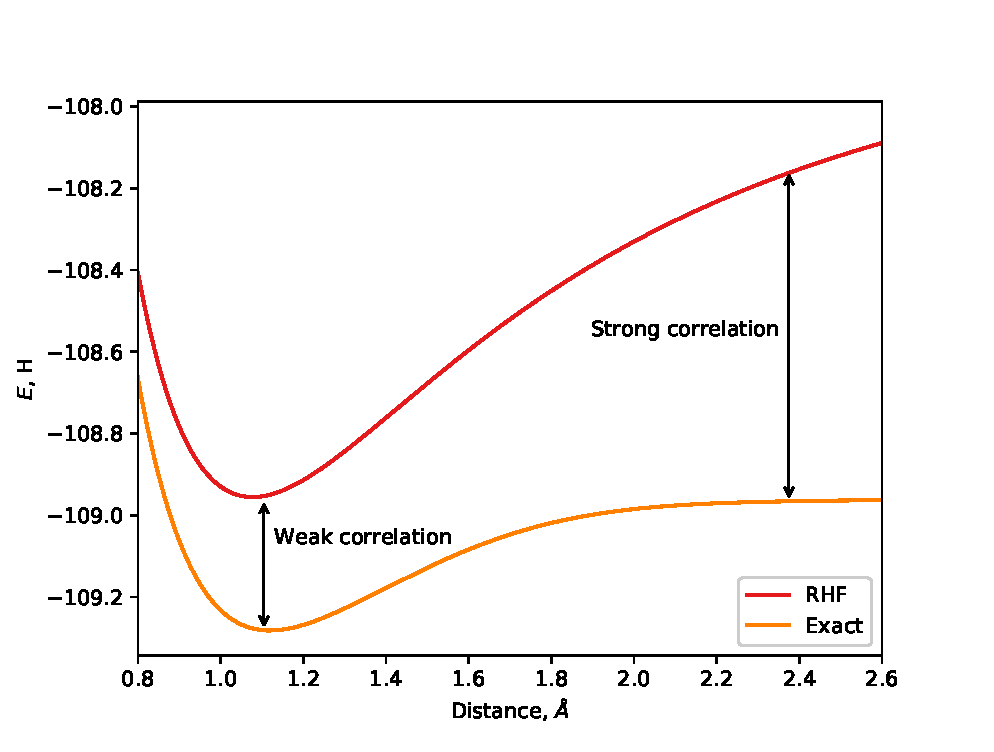
\includegraphics[width=\columnwidth]{figures/prelim/hf_exact}
\caption{Regions of weak and strong correlation along the dissociation 
curve of the nitrogen molecule. RHF refers to restricted Hartree-Fock, exact is 
taken from the exact diagonalization data.
\label{fig:n2_hf_exact}}
\end{figure}
%
Near equilibrium the difference of Hartree-Fock and and exact energies is 
mostly related to short-range dynamical electronic repulsion. When the 
bond is stretched, the bonding, $\sigma^{\ast}_{2p}$ and $\pi_{2p}$ 
orbitals become degenerate, as well as antibonding $\sigma^{\ast}_{2p}$ and 
$\pi_{2p}$ orbitals. Finally, at infinite distance all $2p$ orbitals are the 
same, which leads to the major overestimation of dissociation energy by the HF 
method. Let us now provide some examples of different types of correlation and 
its relation to physical phenomena.

Most correlation in "normal" systems is dynamical. Typical examples 
are usual organic molecules at equilibrium, most metals, semiconductors 
etc. While HF accounts for around $99\%$ of electronic energy, proper 
description of dynamical correlation is crucial in quantitative calculations.
For example, even for atoms, HF excitation energies may be wrong by 
more than $40\%$~\cite{wilson2013methods}, which leads to incorrect prediction 
of ionization potentials. The lack of correlation leads to too short bonds at 
equilibrium, incorrect bond angles, errors in the dipole moments and too high 
harmonic vibrational frequencies.~\cite{helgaker2014molecular, 
scott1996harmonic} HF usually predicts too high reaction barriers, which can be 
understood by the inability of HF to describe stretched bonds. Finally, the 
Hartree-Fock approach is unable to predict pure dispersion 
interaction, correlation bound anions~\cite{voora2013existence} and similar 
systems.

Statically correlated systems are where the shortcomings of Hartree-Fock theory 
are most pronounced, as the independent particle picture becomes inappropriate. 
Static correlation is very common in extended systems and materials 
where $d$- and $f$-electron shells of atoms interact. Among many phenomena 
caused by strong correlation are large resistivity changes, huge volume changes 
across phase transitions, heavy fermion behavior, large 
magnetoresistence and high temperature superconductivity.~\cite{imada1998metal, 
kotliar2004strongly}. Strongly correlated systems are of great importance and 
constant theoretical interest. Accounting for strong correlation is challenging 
for modern electronic structure methods.

As we hope the reader is convinced, the proper description of electronic 
correlation is essential for quantitative many-body simulations. We should now 
follow with the discussion of the approximate many-body methods.

\section{Approximate many-body methods
\label{sec:approx_methods}}
\subsection{Configuration expansion}
As an exact solution of the Schr{\"o}dinger equation can be obtained by 
diagonalizing the Hamiltonian in the basis of all possible determinants, one 
may try to do it over a subset of configurations to save on numerical cost. 
On the other hand, the HF solution $|\Phi_{0}\rangle$ is the best single 
determinant representation of the wavefunction. A natural idea is then to build 
a subset of configurations which are close to $|\Psi_{0}\rangle$:
%
\begin{equation}
\begin{aligned}
 |\Psi \rangle &= u_{0} |\Psi_{0}\rangle + u_{i}^{a} 
c^{\dagger}_{a} c_{i} |\Psi_{0}\rangle + u_{ij}^{ab} c^{\dagger}_{a} 
c^{\dagger}_{b} c_{j} c_{i} |\Psi_{0}\rangle + u_{ijk}^{abc} 
c^{\dagger}_{a} c^{\dagger}_{b} c^{\dagger}_{c} c_{k} c_{j} c_{i} 
|\Psi_{0}\rangle + \ldots \\
 &= \hat{U}_{0} |\Psi_{0}\rangle + \hat{U}_{1} |\Psi_{0}\rangle + \hat{U}_{2} 
|\Psi_{0}\rangle + \hat{U}_{3} 
|\Psi_{0}\rangle \ldots
\end{aligned}
\label{eq:ci_expansion}
\end{equation}
%
Here expansion coefficients $u$ are used for the different orders of 
substituted determinants. We denote occupied HF states by indices 
$i,j,k,\ldots$ and unocupied states by $a,b,c,\ldots$. Note that because 
operators $c$ act in an orthogonal HF basis, all of the terms 
in~\ref{eq:ci_expansion} represent orthogonal configurations. 
Expansion~\ref{eq:ci_expansion} is the basis of many traditional many body 
methods, the simplest example being the Configuration Interaction (CI) method. 
By taking the expectation value of the Hamiltonian with $|\Psi\rangle$ 
and applying the linear variational theorem one ends up with an eigenvalue 
problem for the coefficients $U$:
%
\begin{equation}
 HU = EU
 \label{eq:ci_eigenvalue}
\end{equation}
%
The solution to the above equation provides a variational estimate of 
the energy. It is evident that when all substitutions in $|\Phi_{0}\rangle$ are 
taken we would return to the exact diagonalization, or the full 
configuration interaction (FCI) problem. To make the computation affordable,the 
expansion~\ref{eq:ci_expansion} is usually truncated at double excitations:
%
\begin{equation}
 |\Psi \rangle = u_{0} |\Psi_{0}\rangle + u_{i}^{a} 
c^{\dagger}_{a} c_{i} |\Psi_{0}\rangle + u_{ij}^{ab} c^{\dagger}_{a} 
c^{\dagger}_{b} c_{j} c_{i} |\Psi_{0}\rangle
\end{equation}
%
Truncated CI methods are not very popular in modern calculations. 
Nevertheless, they are used sometimes if excited states are of interest 
and excitation energies need to be 
calculated.~\cite{sherrill1999configuration,head1994doubles}
The problem with the truncated CI approach is that it is neither size 
consistent nor size extensive.~\cite{helgaker2014molecular, 
jensen2017introduction} 

A method is size consistent~\cite{pople1976theoretical} if the energy of two 
non-interacting fragments $A$ and $B$ is the sum of the energies of those 
fragments calculated independently
\begin{equation}
 E(A \overset{d \longrightarrow \infty}{-} B) = E(A) + E(B)
\end{equation}

Size extensivity means that the energy scales linearly with the size of the 
system. For example, the energy of $k$ interacting fragments, such as Helium 
atoms far apart from each other, should equal to the sum of energies of 
individual fragments.
\begin{equation}
 E(k \cdot \mathrm{He}) = k \cdot E(\mathrm{He})
\end{equation}
In thermodynamics extensive quantities scale with the system 
size,~\cite{bartlett1978many} therefore size extensivity is a desirable 
property of any many-body approach.

It turns out that there is a better way of parameterizing the wavefunction in 
the form~\ref{eq:ci_expansion}, which eliminates the drawbacks of CI. This way 
is provided by the coupled cluster ansatz.

\subsection{Coupled Cluster theory}
Since its introduction in nuclear physics,\cite{coester1958bound, 
coester1960short} coupled cluster has become highly popular in quantum 
chemistry due to its exceptional ability to capture weak electronic 
correlation, while still having polynomial computational cost in the size of 
the basis. Another attractive property of CC theory is that while having the 
same number of parameters as CI methods, CC methods are size consistent and 
size extensive\footnote{Coupled cluster is size 
extensive and size consistent only when the reference 
wavefunction has these properties. For example, 
restricted HF-based coupled cluster is not extensive nor consistent in a case 
when an even number of electrons is split into two fragments with an odd number 
of electrons.}, \cite{pople1978electron, 
bartlett1978many, crawford2000introduction, bartlett2007coupled}. In coupled 
cluster the wavefunction is parameterized with an exponential ansatz:
%
\begin{equation}
 |\Psi\rangle = e^{\hat{T}} |\Psi_{0}\rangle
 \label{eq:cc_ansatz}
\end{equation}
Here the excitation operator $\hat{T}$ acts on a reference wavefunction 
$|\Psi_{0}\rangle$ (usually a Hartree-Fock determinant). The excitation 
operator has the same form as in case of CI:
%
\begin{equation}
\begin{aligned}
 \hat{T} &= {}^1\hat{T} + {}^2\hat{T} + {}^3\hat{T} + \ldots \\ 
 &= {}^{1}T_{i}^{a} c^{\dagger}_{a} c_{i} + \frac{1}{4} {}^2T_{ij}^{ab} 
c^{\dagger}_{a} c^{\dagger}_{b} c_{j} c_{i} + \frac{1}{36} {}^3T_{ijk}^{ab} 
c^{\dagger}_{a} c^{\dagger}_{b} c^{\dagger}_{c} c_{k} c_{j} c_{i} 
+\ldots
\end{aligned}
\end{equation}
The coefficient tensors $T$ are called cluster amplitudes. An excitation 
operator of order $n$ is defined by the following expression:
%
\begin{equation}
 {}^{n}\hat{T} = \frac{1}{(n!)^2}{}^{n}T_{ijk\ldots}^{abc\ldots} 
c^{\dagger}_{a} c^{\dagger}_{b} c^{\dagger}_{c} \ldots c_{k} c_{j} 
c_{i} 
\end{equation}
%
The exponential of the excitation operator is understood in terms of a 
polynomial series. Note that in contrast with CI, this ansatz contains not only 
linear excitations, but also products of excitations:
%
\begin{equation}
\begin{aligned}
  & e^{\hat{T}} |\Psi_{0}\rangle = \\
  & (1 + \hat{T} + \frac{1}{2} \hat{T}^{2} + \frac{1}{6} \hat{T}^3 + \ldots) | 
\Psi_{0} \rangle = \\
  & (1 + {}^{1}\hat{T} + \frac{1}{2}({}^{1}\hat{T})^{2} + \ldots + \\
  & {}^{2}\hat{T} + \frac{1}{2}({}^{2}\hat{T})^{2} + \ldots + \\
  & ({}^{1}\hat{T}) ({}^{2}\hat{T}) + \frac{1}{2}({}^{1}\hat{T})^{2} 
({}^{2}\hat{T}) + \ldots) |\Psi_{0} \rangle \\
\end{aligned}
\end{equation}
%
The size extensivity of coupled cluster is a direct consequence of the 
product terms occuring in the exponential function. 

The energy expression can be obtained by inserting~\ref{eq:cc_ansatz} into the 
Schr{\"o}dinger equation:
%
\begin{equation}
 \hat{H} e^{\hat{T}} | \Psi_{0} \rangle  = E |\Psi_{0} \rangle
 \label{eq:half_cc_schroedinger}
\end{equation}
%
This equation, however, can not be solved variationally with low 
cost. The expectation value would be:
%
\begin{equation}
 \frac{\langle \Psi_{0} | e^{\hat{T}^{\dagger}} \hat{H} e^{\hat{T}} | \Psi_{0} 
\rangle}{\langle \Psi_{0} | e^{\hat{T}^{\dagger}} e^{\hat{T}} |\Psi_{0} 
\rangle} = E 
\end{equation}
%
The variational expression above contains all possible excitations up to the 
number of electrons $M$ and no natural truncation scheme exists. 
Solving~\ref{eq:half_cc_schroedinger} variationally thus may not be easier 
than solving the FCI problem. Alternatively, 
Equation~\ref{eq:half_cc_schroedinger} can be solved projectively by 
multiplying it from the left by $e^{-\hat{T}}$:
%
\begin{equation}
 e^{-\hat{T}} \hat{H} e^{\hat{T}} |\Psi_{0} \rangle = E | \Psi_{0} \rangle
\end{equation}
%
The similarity transformed Hamiltonian $\bar{H} = e^{-\hat{T}} \hat{H} 
e^{\hat{T}}$ can be significantly simplified by using 
the Baker-Campbell-Hausdorf (BCH) expansion~\cite{crawford2000introduction, 
shavitt2009many}, which leads 
to nested commutators of the amplitudes and the Hamiltonian:
%
\begin{equation}
\begin{aligned}
  &e^{-\hat{T}} \hat{H} e^{\hat{T}} = \hat{H} + \left[ \hat{H}, \hat{T} \right] 
+ \frac{1}{2!} \left[ \left[ \hat{H}, \hat{T} \right], \hat{T} \right] +\\
&\frac{1}{3!} \left[ \left[ \left[  \hat{H}, \hat{T} \right], \hat{T} \right], 
\hat{T} \right] + \frac{1}{4!} \left[ \left[ \left[ \left[ \hat{H}, \hat{T} 
\right], \hat{T} \right], \hat{T} \right], \hat{T} \right] + \ldots
\end{aligned}
\label{eq:bch_expansion}
\end{equation}
%
Here $\left[ \hat{H}, \hat{T} \right] = \hat{H} \hat{T} - \hat{T}\hat{H}$.
To evaluate the BCH expansion one needs to start with the Hamiltonian in the 
HF basis. The transformation of the Hamiltonian to the mean field basis can 
be done by using operator algebra (see, for example 
Ref.~\cite{crawford2000introduction} for a complete derivation of this 
expression):
%
\begin{equation}
 \hat{H} = E_{0} + F_{q}^{p} c^{\dagger}_{p} c_{q} + \frac{1}{4} (V_{rs}^{pq} 
- V_{sr}^{pq}) c^{\dagger}_{p} c^{\dagger}_{q} c_{r} c_{s}
\end{equation}
%
Here $E_{0}$ is the Hartree-Fock energy, $F$ is a Fock matrix 
(see~\ref{eq:hf_roothaan}), and $V$ is the two electron interaction in the 
molecular orbital basis. The indices $p,q,r,s,\ldots$ in the Hamiltonian are 
general indices, e.g. they run over both occupied and virtual spaces.

By using the commutator arithmetic~\cite{shavitt2009many} it can be shown that 
each commutator between $\hat{H}$ and $\hat{T}$ transforms one general index 
of the Hamiltonian into a Kronecker delta function. As the Hamiltonian has only 
four different general operators, there can only be four commutators with 
$\hat{T}$, and the BCH expansion naturally truncates after the fifth term in 
Eqn.~\ref{eq:bch_expansion}. The similarity transformed Hamiltonian $\bar{H}$ 
will thus be a polynomial of up to fourth order in excitation operators 
$\hat{T}$.

After using the BCH expansion, we are finally in a position to formulate a 
general coupled cluster method. The similarity transformed Schr{\"o}dinger 
equation is:
%
\begin{equation}
 e^{-\hat{T}} \hat{H} e^{\hat{T}} |\Psi_{0}\rangle = E |\Psi_{0}\rangle
 \label{eq:sim_cc_schroedinger}
\end{equation}
It is obvious that the energy can be extracted by taking an expectation value 
with $\langle \Psi_{0}|$. The energy equation is:
%
\begin{equation}
 E = \langle \Psi_{0} | \bar{H} | \Psi_{0} \rangle
 \label{eq:cc_energy}
\end{equation}
The energy expression contains only single (if present in the excitation 
operator $\hat{T}$) and double excitations. Higher orders of 
excitation operator can not be compensated by the Hamiltonian, and would 
necessarily produce orthogonal configurations on the left and right hand sides 
of the expectation value in~\ref{eq:cc_energy}. By using these Slater-Condon 
rules~\cite{jensen2017introduction} the energy of coupled cluster is:
%
\begin{equation}
\begin{aligned}
 E &= \langle \Psi_{0} | (1 - {}^{1}\hat{T} - {}^{2}\hat{T} + \ldots) H (1 + 
{}^{1}\hat{T} + \frac{1}{2} ({}^{1}\hat{T})^2 + \ldots + {}^2 \hat{T} + \ldots) 
= \\
& \langle \Psi_{0} | \hat{H} | \Psi_{0} \rangle + \langle \Psi_{0} | \hat{H} 
({}^{1}\hat{T})| 
\Psi_{0} \rangle + \frac{1}{2} \langle \Psi_{0} | \hat{H} ({}^{1}\hat{T})^2 | 
\Psi_{0} 
\rangle + \langle \Psi_{0} | \hat{H} ({}^{2} \hat{T})| \Psi_{0} \rangle
\end{aligned}
\end{equation}
%
To have a working theory, however, one would need to 
determine cluster amplitudes $\{{}^{1}T, {}^{2}T, {}^{3}T, \ldots$. This can be 
done by projecting the similarity transformed Hamiltonian onto a set of excited 
configurations $\{ \langle \Psi_{i}^{a}, \Psi_{ij}^{ab}, \Psi_{ijk}^{abc}, 
\ldots \}$: 
%
\begin{equation}
\begin{aligned}
 \langle{\Psi_{i}^{a}} | \bar{H} | \Psi_{0} \rangle = 0 \\
 \langle{\Psi_{ij}^{ab}} | \bar{H} | \Psi_{0} \rangle = 0  \\
 \langle{\Psi_{ijk}^{abc}} | \bar{H} | \Psi_{0} \rangle = 0 \\
 \ldots
\end{aligned}
\label{eq:residuals}
\end{equation}
%
The resulting residual equations are polynomial equations for cluster 
amplitudes. Note that because the projection is done with excited 
configurations on the right, these equations can contain higher than double 
amplitudes. In effect, the $n$-th order residual equation would contain 
amplitudes of order $n + 2$ (if they were present in cluster operator), in 
contrast with the energy expression. The inclusion of higher order amplitudes 
into $\hat{T}$ affects the energy only indirectly through corrections to 
singles and doubles. The coupling of residual equations is what gave the name 
to the coupled cluster theory.

If the excitation operator $\hat{T}$ contained all possible orders of 
excitations~$\{ {}^{1}\hat{T}, {}^{2}\hat{T}, \ldots \}$, 
the coupled cluster would be equivalent to exact diagonalization. To have a 
practical method one needs to truncate $\hat{T}$. The energy expression 
justifies the usual truncation of the cluster operator 
$\hat{T}$ at doubles, e.g.:
%
\begin{equation}
 \hat{T} =  {}^{1}T_{i}^{a} c^{\dagger}_{a} c_{i} + \frac{1}{4} {}^2T_{ij}^{ab} 
c^{\dagger}_{a} c^{\dagger}_{b} c_{j} c_{i}
\end{equation}
%
The order of excitation operator $\hat{T}$ determines the name of a particular 
coupled cluster method, with \textbf{S} meaning singles, \textbf{D} denoting 
doubles, \textbf{T} referring to triples etc. Note that by construction CCSD is 
exact for 2-electron systems, CCSDT is exact for 3-electron systems and so on. 
The effect of including single excitations on the accuracy of coupled cluster 
is usually not large, and hence they can often be omitted resulting in the 
simpler coupled cluster with doubles (CCD) method. The cost of coupled cluster 
rises quickly with the order of excitation operator, being of order $O(N^6)$ 
for CCSD, $O(N^8)$ for CCSDT and $O(N^{10})$ for CCSDTQ (see 
chapter~\ref{ch:tcc} for a detailed discussion).

With this result all basic components of a 
general coupled cluster method are set. We will go on to describe a 
particular method used in this work in the next section as well as the procedure 
of finding cluster amplitudes.

%\subsection{Restricted coupled cluster framework}
%Let us describe the restricted coupled cluster methods. Restricted CC uses a 
%spin-adapted Hartree-Fock configuration $|\Psi_{0} \rangle$ as a reference. 
%This means that $|\Psi_{0}\rangle$ is an eigenfunction of the $\hat{S^2}$ and 
%$\hat{S_z}$ operators, and hence has a definite total spin and $s_{z}$ quantum 
%numbers. Spin is a symmetry in molecular systems, as spin operators commute 
%with the Hamiltonian. It was L{\"o}wdin~\cite{carlos_16} who first 
%demonstrated that breaking symmetries in HF can remove degeneracy of single 
%determinant 
%configurations and yield lower energy solutions. Broken 
%symmetry wavefunction, however, have many undesirable features: they may not 
%be continuous with respect to the parameters of the Hamiltonian (this 
%manifests 
%as discontinuities on potential energy surfaces~\cite{tom_ghf}), the 
%spin-density is wrong etc.
%
%A consistent way for preserving physical symmetries 
%of the Hamiltonian and yet having a high quality wavefunction was introduced 
%in 
%the works of Jim{\'e}nez-Hoyos, Scuseria \emph{et al.} in their Projected 
%Hartree-Fock method.~\cite{} Later, this methodology was imported to the 
%context of Coupled Cluster theory by Henderson, Qui, Scuseria and coworkers 
%in a series of works.~\cite{} We would omit the discussion of these 
%potent methods here to not digress from the main topic of the section. We 
%should remark, however, that improving these perspective techniques with the 
%the ideas introduces in this manuscript is one of the future avenues of our 
%research.
%
%As we said, we chose to work in a spin restricted framework here. The 
%spin-preserving cluster amplitudes can be pameterized with the following 
%spin-adapted operators~\cite{scuseria}:
%%
%\begin{equation}
% e_{i}^{a} = \frac{1}{2}(c^{\dagger}_{a, \uparrow} c_{i, \uparrow} + 
%c^{\dagger}_{a, \downarrow} c_{i, \downarrow}) 
%\end{equation}
%%
%Here distinct labels are introduced for the spatial and spin index of the 
%single particle basis. The operator $c^{\dagger}, \uparrow$ creates an 
%electron on the $i$-th orbital with a $z$-projection of spin being up. The 
%spin-adapted cluster operators are:
%%
%\begin{equation}
%\begin{aligned}
% & \hat{T} = {}^{1}T_{i}^{a} e_{i}^{a} + \frac{1}{2} {}^{2}T_{ij}^{ab} 
%e_{i}^{a} e_{j}^{b} + \ldots \\
% = {}^{1} T_{i}^{}
%\end{aligned}
%\end{equation}
%%
%Note that these expressions contain less parameters that the excitation 
%operator would do, and hence the amplitude tensors have to have certain 
%symmetries.

\subsection{Restricted Coupled Cluster Doubles (RCCD)
\label{sec:preliminaries_rccd}}
The coupled cluster theory we introduced so far is the most general case 
possible. For closed shell systems as we used in this work, we can 
realize significant computational savings by using the property that our 
orbitals are doubly occupied. This assumption also guarantees that we preserve 
a proper spin symmetry in our restricted CC wavefunction. The drawback of this 
ansatz is that the restricted Hartree-Fock wavefunction $|\Psi_{0}\rangle$ 
will become degenerate when energy levels of opposite spin 
electrons become equivalent. This degeneracy (or strong correlation)
will cause a failure of the restricted CC methods, which we will address at the 
end of Chapter~\ref{ch:app_tcc}. For more information on the 
connection of symmetries and strong correlation please see 
Refs.~\cite{jimenez2012projected, scuseria2011projected} and the book of Ring 
and Schuck~\cite{ring2004nuclear}. The ideas described in 
the next chapter do not depend on the choice of the ansatz.

The actual residual equations in RCCD (see Eqn.~\ref{eq:residuals}) can be 
derived either by employing Slater-Condon rules to evaluate the matrix elements 
or by algebraic techniques employing second quantization. The derivation 
involves a significant amount of algebra and therefore will be 
omitted here. A detailed summary of these techniques can be found in 
Refs.~\cite{crawford2000introduction, shavitt2009many}. The final RCCD energy 
equation is shown below:
%
\begin{equation}
 E = E_{0} + {}^{2} T^{ab}_{ij} \cdot (2 \cdot V^{ij}_{ab} - V^{ij}_{ba})
\label{eq:ccd_energy_equation}
\end{equation}
%

The ${}^2 T$ residual equation has the following form:
\begin{equation}
\begin{split}
0 & = R^{ab}_{ij} = -V^{ab}_{ij} \\
& + {}^{2}T^{ab}_{kj} F^{k}_{i} 
+ {}^{2}T^{ab}_{ik} F^{k}_{j}
- {}^{2}T^{cb}_{ij} F^{a}_{c} 
- {}^{2}T^{ac}_{ij} F^{b}_{c} \\
& - {}^{2}T^{cd}_{ij}  V^{ab}_{cd}
+ {}^{2}T^{ac}_{ik}  V^{bk}_{cj} 
+ {}^{2}T^{ac}_{ki}  V^{bk}_{jc} 
+ {}^{2}T^{ac}_{kj}  V^{bk}_{ci} 
+ {}^{2}T^{cb}_{kj}  V^{ak}_{ci}\\
&+ {}^{2}T^{bc}_{ki}  V^{ak}_{cj} 
+ {}^{2}T^{bc}_{kj}  V^{ak}_{ic}
- 2 \cdot {}^{2}T^{ac}_{ik}  V^{bk}_{jc}
- 2 \cdot {}^{2}T^{bc}_{jk}  V^{ak}_{ic}
- {}^{2} T^{ab}_{kl}  V^{kl}_{ij} \\
&- {}^{2} T^{ab}_{ik}  ({}^{2} T^{cd}_{lj})  V^{kl}_{cd} 
- {}^{2} T^{ab}_{kj}  ({}^{2} T^{cd}_{il}) V^{kl}_{dc}
- {}^{2} T^{ab}_{kl}  ({}^{2} T^{cd}_{ij}) V^{kl}_{cd}
- {}^{2} T^{ac}_{ij}  ({}^{2} T^{bd}_{kl})  V^{kl}_{dc}
-  {}^{2} T^{ac}_{ik}  ({}^{2} T^{bd}_{lj}) V^{kl}_{dc} \\
&- {}^{2} T^{ac}_{ki}  ({}^{2} T^{bd}_{jl}) V^{kl}_{dc}
- {}^{2} T^{ac}_{ki}  ({}^{2} T^{bd}_{lj}) V^{kl}_{cd}
- {}^{2} T^{ac}_{kj}  ({}^{2} T^{bd}_{li}) V^{kl}_{dc}
-  {}^{2} T^{ac}_{kl}  ({}^{2} T^{bd}_{ji}) V^{kl}_{cd}
+ 2 \cdot {}^{2} T^{ab}_{ik} ({}^{2} T^{cd}_{lj})  V^{kl}_{dc}\\
&+ 2 \cdot {}^{2} T^{ab}_{kj} ({}^{2} T^{cd}_{il})  V^{kl}_{cd}
+ 2 \cdot {}^{2} T^{ac}_{ij} ({}^{2} T^{bd}_{kl})  V^{kl}_{cd}
+ 2 \cdot {}^{2} T^{ac}_{ik} ({}^{2} T^{bd}_{jl})  V^{kl}_{dc}
+ 2 \cdot {}^{2} T^{ac}_{ik} ({}^{2} T^{bd}_{lj})  V^{kl}_{cd}\\  
&+ 2 \cdot {}^{2} T^{ac}_{ki} ({}^{2} T^{bd}_{jl})  V^{kl}_{cd}
+ 2 \cdot {}^{2} T^{ac}_{kl} ({}^{2} T^{bd}_{ji})  V^{kl}_{dc}
- 4 \cdot {}^{2} T^{ac}_{ik} ({}^{2} T^{bd}_{jl})  V^{kl}_{cd})
\end{split}
\label{eq:ccd_amplitude_equation}
\end{equation}  
As was noted in the previous section, this is a polynomial equation 
for the amplitude tensor ${}^2T$. The right hand side of the residual 
$R_{ij}^{ab}$ contains a constant (driving) term $V_{ij}^{ab}$, terms linear in 
the amplitudes ${}^2T$ and quadratic terms. A classical way of 
solving~\ref{eq:ccd_amplitude_equation} is by splitting the residual 
expression to extract the amplitude tensors. In particular, the diagonal part 
of the summations containing Fock matrices can be separated as follows:
%
\begin{equation}
\begin{aligned}
 & {}^2T_{ij}^{ab} (F_{a}^{a} + F_{b}^{b} - F_{j}^{j} - F_{i}^{i}) = \\
 & \sum_{k\neq i} {}^{2}T^{ab}_{kj} F^{k}_{i}
+ \sum_{k \neq j} {}^{2}T^{ab}_{ik} F^{k}_{j}
- \sum_{k \neq a} {}^{2}T^{cb}_{ij} F^{a}_{c}
- \sum_{k \neq b} {}^{2}T^{ac}_{ij} F^{b}_{c} + \mathrm{the~rest} 
\end{aligned}
\label{eq:ccd_splitting}
\end{equation}
%
By denoting the right hand side of the above expression by ${}^{2}G_{ij}^{ab}$, 
the working expressions for the RCCD method can be formulated:
%
\begin{equation}
{}^{2}T_{ij}^{ab} = {}^{2}D_{ij}^{ab} ~ {}^{2}G_{ij}^{ab}
\label{eq:ccd_amplitude_equation_short}
\end{equation}
%
Here $D$ is the denominator tensor, which is usually present in coupled cluster 
and perturbation theories.
%
\begin{equation}
 {}^{2}D_{ij}^{ab} = \frac{1}{F_{a}^{a} + F_{b}^{b} - F_{j}^{j} - 
F_{i}^{i}}
\label{eq:cc_denom_definition}
\end{equation}
As amplitude equations 
\ref{eq:ccd_amplitude_equation_short} are 
not linear, they are usually solved by iteration. In the first iteration all 
entries in the amplitude tensor are set to zero: ${}^{2}T_{ij}^{ab} = 0$. This 
only leaves the two body interaction term, and the initial ${}^2T$ amplitudes 
are 
obtained as:
%
\begin{equation}
 {}^{2}{T_{ij}^{ab}}^{(1)} =  \frac{-V^{ab}_{ij}}{F_{a}^{a} + F_{b}^{b} - 
F_{j}^{j} - F_{i}^{i}}
\end{equation}
%
Note that the energy calculated with these first step amplitudes is exactly the 
same as in (restricted) second order perturbation theory (MP2).
%
\begin{equation}
 E = E_{0} -  \frac{V^{ab}_{ij} \cdot (2 V^{ij}_{ab} - 
V^{ij}_{ba})}{F_{a}^{a} + F_{b}^{b} - 
F_{j}^{j} - F_{i}^{i}}
\end{equation}
%
This is a consequence of a connection between coupled cluster and perturbation 
theory, and allows one to calculate MP2 energies as a byproduct of the coupled 
cluster procedure. Coupled cluster, however, is usually superior to the 
perturbation theory methods. 

So far we introduced the simplest coupled cluster model and have shown a way to 
find cluster amplitudes. All calculations done in this work also included 
single excitations in the cluster operator, although we use a simpler RCCD 
approach to describe our approximate CC methods in Chapter~\ref{ch:tcc}. A more 
general RCCSD method is briefly explained in the next section.

\subsection{Restricted Coupled Cluster Singles and Doubles (RCCSD)
\label{sec:preliminaries_rccsd}}
While being the simplest Coupled Cluster method to implement, RCCD does not 
offer very high accuracy. The inclusion of single excitations in the cluster 
operator improves the precision by accounting for the 
relaxation effects in the reference determinant. The RCCSD method is quite 
accurate, especially if large basis sets are used. Typical errors in predicted 
bond lengths are of order of $0.5$ pm~\cite{coriani2005accuracy}, and the 
reaction enthalpies are usually accurate up to $\sim 10$ 
kJ/mol~\cite{bak2000accuracy}.

The energy expression in RCCSD contains contributions from singles amplitudes:
%
\begin{equation}
E = E_{0} + {}^{2}T^{ab}_{ij} \cdot(2 \cdot  
V^{ij}_{ab} - V^{ij}_{ba})  + 2 F^{i}_{a}  {}^{1}T^{a}_{i} 
+ {}^{1}T^{a}_{i} ({}^{1}T^{b}_{j}) \cdot (2 \cdot V^{ij}_{ab} - 
V^{ij}_{ba})   
\end{equation}
%
The amplitude equations in RCCSD are analogous to RCCD and can be found in 
Ref.~\cite{shavitt2009many}. We will not list these equations here 
due to their length. Symbolically, the amplitude equations are
\begin{subequations}
\begin{equation}
{}^{1}T_{i}^{a} = {}^{1}D_{i}^{a} ~ {}^{1}G_{i}^{a} \\
\end{equation}
\begin{equation}
{}^{2}T_{ij}^{ab} = {}^{2}D_{ij}^{ab} ~ {}^{2}G_{ij}^{ab}
\label{eq:ccsd_amplitude_equation_short}
\end{equation}
\end{subequations}

Where  ${}^{1}D_{i}^{a} = \frac{1}{F_{a}^{a} - F_{i}^{i}}$, ${}^{1}G$ is 
the right hand side in singles residual equation, and other terms are 
analogous to RCCD. The doubles right hand side ${}^{2}G$ in RCCSD contains all 
terms present in RCCD plus additional terms contributed by singles.

Solving the doubles amplitude equations is computationally demanding, 
and determines the very steep cost of RCCD and RCCSD approaches. The evaluation 
of the right hand side of Eq. \ref{eq:ccsd_amplitude_equation_short} requires 
$O(N^6)$ summations and multiplications per iteration, hence the RCCSD method 
has $O(N^6)$ cost. The root of this problem is the need to perform summations 
involving fourth order tensors representing the interaction $V$ and 
excitation amplitudes. This problem, however, can be circumvented by using 
novel techniques of tensor decompositions coming from multilinear 
algebra,\cite{kolda2009tensor} as we will demonstrate in the next chapter.

\section{Solvable models
\label{sec:hubbard_hamiltonian}}
As was said before, all many body methods serve the purpose of finding 
(approximate) eigenfunctions of the Hamiltonain. For certain 
Hamiltonians exact solutions can be found without reverting to direct 
diagonalization.\cite{dukelsky2004colloquium} Those solvable models are often 
used to benchmark many-body approaches.

One of the widely used models is the one-dimensional Hubbard 
Hamiltonian, whose eigenfunctions can be produced by solving Lieb-Wu 
equations.\cite{lieb1968absence} This Hamiltonian can be regarded as a 
simplified representation of a collection of hydrogen atoms located in a 
ring, where only one basis function per atom is used to describe the system, 
and only the Coulomb repulsion within the atom is taken into account. 
The Hamiltonian is:
\begin{equation}
 H = - t \sum_{\mu, \sigma} (a^\dagger_{\mu + 1, \sigma} a_{\mu, 
\sigma} + a^\dagger_{\mu, \sigma} a_{\mu + 1, 
\sigma}) + u \sum_{\mu} a^\dagger_{\mu, \uparrow} a^\dagger_{\mu, \downarrow} 
a_{\mu, \downarrow} a_{\mu, \uparrow}
\end{equation}
Here, $a^\dagger_{\mu}$ creates an electron on site $\mu$ of the lattice with 
$\sigma = \{ \uparrow, \downarrow \}$ $z$-projection of
spin. The scalar $t$ sets the energy gain from hopping of electrons to neighbor 
sites, while $u$ is the strength of repulsion of opposite spin electrons 
at the same site. Usually periodic boundary conditions are implied, which means 
that in $N$-site system the site $N + k$ is equivalent to site $k$.

Despite its simple structure, the Hubbard model describes both weak and strong 
correlation regimes depending on the ratio of potential and kinetic energy 
terms $\eta = u / t$. For low values of $\eta \sim 1$ the ground state is 
weakly correlated, while as $u / t$ grows the solutions of the model may be 
strongly correlated. The simulation of the Hubbard Hamiltonian is usually done 
at half-filling, e.g. when the total number of electrons equals the number of 
sites. At half-filling $N$ one particle configurations are degenerate at $\eta 
>> 0$, which leads to strong correlation. We refer the reader to 
Ref.~\cite{essler2005one} for a complete review of the Hubbard model.

\chapter{Tensor Structured Coupled Cluster
\label{ch:tcc}} 
The discussion presented in this section is based on our published work, see 
Ref.~\cite{schutski2017tensor}, and also on several new results intended for 
another publication.

\section{Tensor Contractions and the Cost of Coupled Cluster}
Our goal here is to improve the very steep cost of the coupled 
cluster method. The numerical cost of CC methods lies in solving amplitude 
equations. We will show how to reduce this effort by two orders of 
magnitude by introducing alternative representations of the Hamiltonian 
and amplitude tensors. But first, let us look back at some of the terms in the 
RCCD amplitude equation:
%
\begin{equation}
\begin{split}
T^{ab}_{ij} & = D^{ab}_{ij} \cdot (- V^{ab}_{ij} \\
& + \sum_{k \neq i} F^{k}_{i} T^{ab}_{kj}
+  \sum_{k \neq j} F^{k}_{j}  T^{ab}_{ik}
- \sum_{c \neq a} F^{a}_{c}  T^{cb}_{ij}
- \sum_{c \neq b} F^{b}_{c}  T^{ac}_{ij} \\
& - T^{cd}_{ij}  V^{ab}_{cd}
+ T^{ac}_{ik}  V^{bk}_{cj} 
+ T^{ac}_{ki}  V^{bk}_{jc} 
+ T^{ac}_{kj}  V^{bk}_{ci} 
+ T^{bc}_{jk}  V^{ak}_{ci}\\
&+ \mathrm{other~terms}
\end{split}
\label{eq:ccd_amplitude_equation_head}
\end{equation}
%
Again, here $F$ is the Fock matrix, $V$ is the electron interaction tensor in 
the molecular orbital basis (Dirac ordered) and $D$ is an orbital energy 
denominator. Most of the terms on the right hand side of 
Eqn.~\ref{eq:ccd_amplitude_equation_head} are numerically expensive to 
evaluate. For example, the second term containing interaction 
$V$ is
%
\begin{equation}
 \tau^{ab}_{ij} = T^{ac}_{ik}  V^{bk}_{cj}
 \label{eq:ccd_intermediate_example}
\end{equation}
%
This expression requires $O(N^6)$ multiplications and additions, as for every 
one of the $N^4$ elements in the intermediate $\tau$ one has to calculate $N^2$ 
products and sums. To facilitate the discussion and the estimates of cost let 
us introduce a graphical notation for tensors:
%
\begin{equation}
\vcenter{\hbox{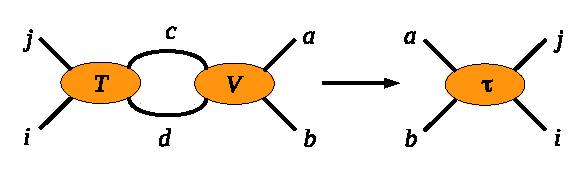
\includegraphics[width=0.6\textwidth]
{figures/tcc_theory/cc_contraction_1} } }
.
\label{fig:cc_contraction_1}
\end{equation}
%
In this notation we represent tensors by shapes, and their 
indices by lines. Open lines denote free indices, and connected lines mean a
contraction over respective indices. If each index had a size proportional to 
$N$, one can then estimate the cost of the contraction as $N^{K}$, where the 
exponent $K$ is the sum of the number of open lines in the result and 
the number of connected lines. Thus, the cost scales as $N^6$ in 
Eqn.~\ref{fig:cc_contraction_1}. For more examples of the graphical notation 
please see Appendix~\ref{sec:graphical_notation}. We will omit index 
letters on most further diagrams.

The very same contraction can be evaluated with lesser effort if the electron 
interaction tensor is approximated by a well known\cite{beebe1977, 
vahtras1993integral, boman2008method, sierka2003fast} resolution of identity 
(RI) decomposition:
%
\begin{equation} V^{pq}_{rs} \approx \sum_{\alpha \alpha^{\prime}} 
U_{pr}^{\alpha}
D_{\alpha,\alpha^{\prime}} \tilde{U}_{qs}^{\alpha^{\prime}},
\label{eq:ri_decomposition}
\end{equation}
Here $U$ and $\tilde{U}$ are three index-integrals and $D$ is a generalized 
overlap.\cite{ahmadi1995coulomb}. The resolution of identity can be 
seen as a singular value or an eigenvalue decomposition of the 
interaction tensor. If tensor $V^{pq}_{rs}$ is reshaped into a matrix with 
combined indices $pr$ and $qs$, then three index tensors $U$ and $\tilde{U}$ are 
its singular vectors (or eigenvectors), and $D$ is a diagonal matrix of 
singular values (or eigenvalues). The RI decomposition, however, does not 
enforce in general that $U$ and $\tilde{U}$ are orthogonal or that $D$ is 
diagonal.

The accuracy of the decomposition in Eqn.~\ref{eq:ri_decomposition}
will depend on the size of the introduced index $\{ \alpha \}$, called the rank 
of RI, or the size of the auxiliary basis. It is well known that the error of 
RI decreases exponentially with the size of $\{ \alpha \}$. Negligible errors 
are attained with $dim(\{ \alpha \}) = r_{RI} = O(N)$.\cite{beebe1977, 
sierka2003fast} Diagrammatically, Eqn.~\ref{eq:ri_decomposition} is
%
\begin{equation}
\vcenter{\hbox{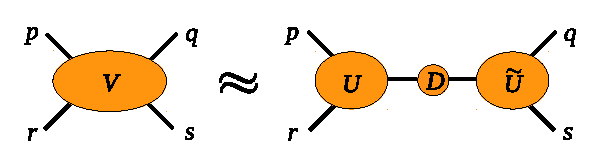
\includegraphics[width=0.6\textwidth]
{figures/tcc_theory/ri_decomposition}}}.
\label{fig:ri_decomposition}
\end{equation}
%
By using the RI decomposition the intermediate in 
Eqn.~\ref{fig:cc_contraction_1} can be formed at $O(N^5)$ cost, 
as shown on the diagram below:
%
\begin{equation}
\vcenter{\hbox{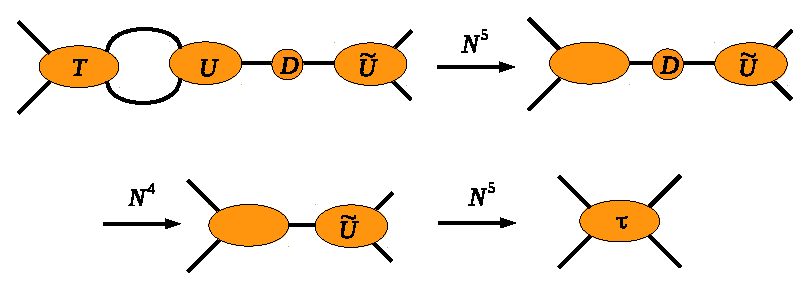
\includegraphics[width=0.6\textwidth]
{figures/tcc_theory/cc_contraction_2}}}.
\label{fig:cc_contraction_2}
\end{equation}
%
The RI decomposition has been used for a long time to reduce the
scaling of quantum chemistry algorithms, for example, in the RI-MP2
method.\cite{ayala1999linear, werner2003fast, izmaylov2008resolution} A 
significant caveat is, however, that while keeping the dimension of the 
auxiliary basis low, one can only 
separate a pair of indices $p, r$ 
from another pair $q, s$ with good accuracy, but not $p, q$ from $r, s$. 
In the latter case the rank of RI has to be $r_{RI} = O(N^2)$ instead of 
$r_{RI} = O(N)$ to provide equivalent accuracy. The approximation in the last 
case would be not useful, because RI factors would contain almost the same 
number of elements as the original tensor. Those 
properties of RI are apparent from the form of the electron interaction 
operator:
%
\begin{equation}
%\begin{split}
 V^{pq}_{rs} = \int \frac{\phi^{\star}_{p}(\vec{r}_{1}) 
\phi^{\star}_{q}(\vec{r}_{2}) \phi_{r}(\vec{r}_{1}) \phi_{s}(\vec{r}_{2})}{| 
\vec{r}_{1} - \vec{r}_{2} |} 
d\vec{r}_{1} d\vec{r}_{2} \\ 
%& \approx \int \phi^{\ast}_{p}(r_{1}) \phi_{r}(r_{1}) \chi_{\alpha}(r_{1}) 
%dr_{1} 
%\int \phi^{\ast}_{q}(r_{2}) \chi_{s}(r_{2}) \psi_{\alpha^{\prime}}(r_{2}) 
%dr_{2} \\ & \cdot \int \frac{\chi_{\alpha}(r_{1}) 
%\chi_{\alpha^{\prime}}(r_{2})}{| r_{1} - 
%r_{2} |} dr_{1} dr_{2}
%\end{split}
\label{eq:ri_decomposition_integral}
\end{equation}
%
As Eqn.~\ref{eq:ri_decomposition_integral} implies, a separation of variables 
between a pair of basis functions $p, r$ and $q, s$ is possible when the 
distance $|\vec{r}_{1} - \vec{r}_{2}|$ is large. In contrast, this is not true 
for pairs $p, q$ and $r, s$ in $V^{pq}_{rs}$.

This limitation of the RI decomposition does not allow cost reduction during 
the calculation of several terms in the residual equation of RCCD. For example, 
the evaluation of the 6th term Eqn.~\ref{eq:ccd_amplitude_equation}:
%
\begin{equation}
 \tau^{ab}_{ij} = - T^{cd}_{ij}  V^{ab}_{cd}
 \label{eq:ccd_intermediate_example2}
\end{equation}
%
does not benefit from RI decomposition of $V$.
%
\begin{equation}
\vcenter{\hbox{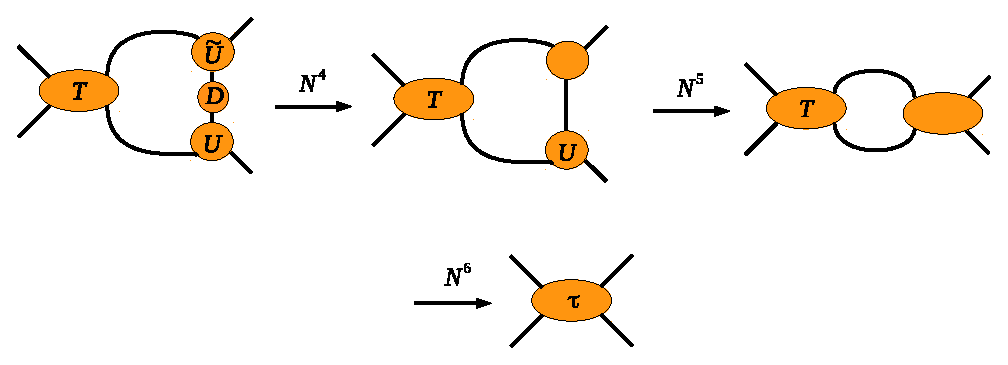
\includegraphics[width=0.8\textwidth]
{figures/tcc_theory/cc_contraction_3}}}
.
\end{equation}
%
Further approximations, however, can lead to lower cost of this expression.

\section{Tensor decompositions}
As was noted before, the simple RI approximation may not always reduce the 
computational cost. To build a more flexible approximation of the interaction 
tensor we need to consider additional tensor decompositions. In this section we 
will only briefly list the decompositions we used, and refer the reader to 
the original publications for technical details. The important information here 
is the structure of the described factorizations, which we demonstrate using 
tensor diagrams. Another important aspect is the alternating least squares 
method (ALS), as it can be used to calculate \emph{any} of the described 
decompositions and is a cornerstone of our factorized CC approaches.

\subsection{Canonical Polyadic Decomposition}
An $n$-dimensional tensor can always be produced as a result of the direct 
product of $n$ vectors. In the simplest case of the three dimensional tensor 
with one vector per each dimension we would have:
%
\begin{equation}
\tau = a \times b \times c 
\end{equation}
%
These tensors are called elementary rank-1 tensors or polyads. The Hartree-Fock 
method can be regarded as minimization of the energy functional over 
wavefunctions being a single polyad (over antisymmetric vector spaces and with 
an additional constraint of vectors to be orthogonal and normalized). General 
tensors, however, can be expressed as sums 
of polyads~\cite{hackbusch2014numerical} 
(again, compare this to correlated wavefunctions in many-body theory, which may 
be expressed as sums of Slater determinants):
%
\begin{equation}
 T = \sum_{\alpha} \tau^{\alpha}
\end{equation}
%
The polyadic decomposition~\cite{de2006link} of a tensor is thus a decomposition 
of the form:
%
\begin{equation}
T_{pqr\ldots} = \sum_\alpha a_p^\alpha \, b_q^\alpha \,
c_r^\alpha \ldots
\label{eq:cpd_definition}
\end{equation}
%
The dimension of the auxiliary index $\alpha$ is called the 
rank of the decomposition. As the rank is increased, this decomposition can 
approximate an arbitrary tensor with any given precision. The factorization with 
the lowest possible rank is called canonical polyadic decomposition (CPD), but 
we would omit this detail and call CPD any decomposition of the form shown in 
Eqn.~\ref{eq:cpd_definition}. The CPD of a three index tensor is shown below 
diagrammatically.
\begin{equation}
\vcenter{\hbox{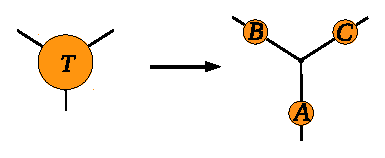
\includegraphics[width=0.4\textwidth]
{figures/tcc_theory/cp_decomposition}}}
.
\label{fig:cp_decomposition}
\end{equation}
%
This factorization can be seen as one of the generalizations of classic 
decompositions of matrices, such as QR, LU or Singular Value Decomposition, to 
higher order tensors.\cite{kolda2009tensor} The important 
difference, is, however, that no closed form algorithm to extract the CPD for 
generic tensors is known, and one has to rely on iterative optimization 
techniques.\cite{sorber2013optimization} 

Substantial effort has been made by the mathematical community to develop 
optimization techniques for CPD. We refer the reader to the corresponding 
reviews~\cite{kolda2009tensor, sidiropoulos2016tensor} for further details. 
Typical algorithms are the alternating least squares 
(ALS),\cite{comon2009tensor} gradient descent by 
means of the method of Broyden, Fletcher, Goldfarb, and Shanno 
(BFGS), and nonlinear least squares (NLS) methods.\cite{sorber2013optimization}

\subsubsection{Analytical Canonical Decomposition}
For a limited number of special tensors the CPD can be built analytically. 
One such case are tensors which can be expressed in the form:
%
\begin{equation}
T_{abc\ldots} = 
f(x_{a} + y_{b} + z_{c} + \ldots)
\end{equation}
%
Here $f$ is an arbitrary differentiable function, and $x_{a}$ are values of the 
argument on a finite interval. CP decomposition for these tensors can be 
built using an exponential parameterization.\cite{braess2005approximation} We 
note that the denominator tensors in coupled cluster theories (see Section 
\ref{sec:preliminaries_rccd}) have a suitable structure: 
%
\begin{equation}
D^{ab\ldots}_{ij\ldots} = 
\frac{1}{F_{a}^{a} + F_{b}^{b} + \ldots - F_{i}^{i} - 
F_{j}^{j} - \ldots}
\end{equation}
CPD of energy denominator tensors was known as Laplace 
transformation in quantum chemistry for a long 
time.\cite{almlof1991elimination} The exponential parameterization of the 
denominator tensors is:
%
\begin{subequations}
\begin{align} {}^2D_{ij}^{ab} &= 
\sum_{\omega} C_\omega \, \mathrm{e}^{A_\omega \,
F_i^i} \, \mathrm{e}^{A_\omega \, F_j^j} \, \mathrm{e}^{-A_\omega \,
F_a^a} \, \mathrm{e}^{-A_\omega \, F_b^b} \\ &= \sum_{\omega} {}^2D^1_{i,\omega} 
\,
{}^2D^2_{j,\omega} \, {}^2D^3_{a,\omega} \, {}^2D^4_{b,\omega}.
\end{align}
\end{subequations}
%
Quadrature weights $C_{w}$ and coefficients $A_{w}$ in this case can be 
precomputed without knowledge of the individual values of the Fock matrix 
diagonal $F$ (they depend only on the span of the values and a desired 
magnitude of error) and provide very high accuracy of the resulting 
decomposition.\cite{braess2005approximation}
%
\subsubsection{Exact decomposition of sparse tensors}
Another important special case when an exact CPD can be built are very sparse 
tensors. A tensor $T$ having $r$ non zero elements can be represented exactly 
by its trivial CPD of rank $r$, which will take a form
%
\begin{equation}
T_{pqr\ldots} = \sum_{\alpha \in T_{pqr\ldots} \neq 0} \lambda_{p^\alpha 
q^{\alpha} 
r^{\alpha}\ldots} \cdot e^{1}_{p^{\alpha}} \, e^{2}_{q^\alpha} \, 
e^{3}_{r^\alpha} \ldots
\label{eq:trivial_cpd_dec}
\end{equation}
%
where $e^{n}_{p^{\alpha}}$ is a unit vector of the same length as $n$-th 
dimension of $T$ having $1$ in $p^{\alpha}$-th position, and 
$\lambda_{p^{\alpha}q^{\alpha}r^{\alpha}\ldots}$ is a non-zero element of 
$T$. Essentially, CPD in this case is a weighted sum of rank-1 tensors having 
$1$ in a specific entry and 
zeros everywhere else with 
weights corresponding to the values of non-zeros entries in $T$. This 
trivial decomposition may be useful only if the number of non-zero entries of 
$T$, and hence the rank of the CPD, is small. The particular way this trivial 
CPD is built shows an intrinsic connection of the CPD and sparsity.

\subsection{Tensor Hypercontraction}
\label{sec:tensor_hypercontraction}
The resolution of identity, which we considered before, can be combined with 
canonical decomposition. If the three-index tensors in RI are further 
approximated by CPD one comes to a Tensor Hypercontraction (THC) introduced by 
Martinez \emph{et al.}\cite{hohenstein_thc1, hohenstein_thc2, hohenstein_thc3}
The THC is a decomposition of fourth order tensors of the form:
\begin{equation}
\begin{split} V_{pqrs} & = \sum_{\alpha \beta} W^{1}_{p,\alpha} W^{2}_{q, 
\alpha}
X_{\alpha, \beta} W^{3}_{r, \beta} W^{4}_{s, \beta} 
\end{split}
\label{eq:thc_definition}
\end{equation}
Diagrammatically, THC is
\begin{equation}
\vcenter{\hbox{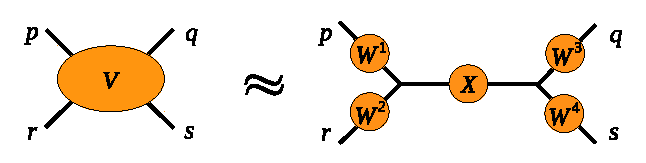
\includegraphics[width=0.5\textwidth]
{figures/tcc_theory/thc_decomposition}}}
.\label{fig:thc_decomposition}
\end{equation}
THC can be seen as a further approximation to RI, which is apparent from the 
following sequence of diagrams:
\begin{equation}
\vcenter{\hbox{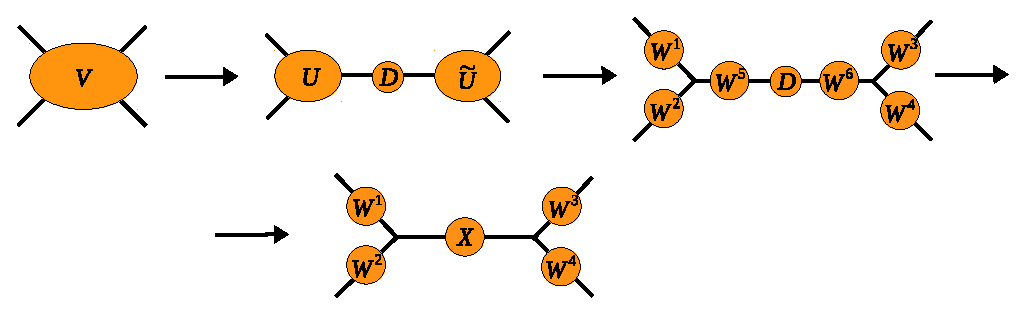
\includegraphics[width=0.8\textwidth]
{figures/tcc_theory/thc_cpd}}}.\label{fig:thc_cpd}
\end{equation}
As those diagrams suggest, THC can be calculated in two steps. First, an RI 
of the original tensor is calculated, and then CP decomposition of the 
three-index tensors is obtained by means of optimization 
algorithms. Finally, the factors without external indices (open lines) 
are contracted together to produce the THC.\cite{hohenstein_thc1}

For the specific case of two electron integrals Martinez \emph{et al.} developed 
fast non-iterative methods where fixed real-space quadratures were used in 
place of factors $W^{1}, W^{2}, W^{3}, W^{4}$.\cite{hohenstein_thc3, 
hohenstein_cc2, parrish2013discrete} This can be compared to obtaining CPD 
analytically, as was mentioned in the previous section.

We also proposed direct optimization methods for calculating THC by alternating 
least squares and gradient descent in our work,\cite{schutski2017tensor} but 
found them inferior to the two step approach originally described by Martinez 
\emph{et al.}.\cite{hohenstein_thc1}

\subsection{Alternating Least Squares}
Let us now describe a general optimization method, which can be applied to 
calculate several tensor decompositions. We will show its derivation for the 
optimization of THC as was done in our original work,\cite{schutski2017tensor} 
but it can be equally used to compute CPD and, possibly, other decompositions.

We start by defining an approximation to a four index tensor $V$ by its THC 
decomposition $\tilde{V}$:
%
\begin{subequations}
\begin{align} \tilde{V}_{ijkl} &= \sum_{\alpha \beta} W^{1}_{p,\alpha} W^{2}_{q, 
\alpha} X_{\alpha, \beta} W^{3}_{r, \beta} W^{4}_{s, \beta} \\
\end{align}
\end{subequations}
%
The element-wise error can be written as
%
\begin{equation}
\Delta_{V} = V - \tilde{V},
\end{equation}
%
the square of the Frobenius norm of this tensor is a sum of its entries squared:
%
\begin{equation} f = \|\Delta_V\|^2 = \sum_{pqrs} \left(V^\ast_{pqrs} -
\tilde{V}^\ast_{pqrs}\right) \, \left(V_{pqrs} -
\tilde{V}_{pqrs}\right).
\label{eq:cost_function}
\end{equation}
%
Diagrammatically, the latter expression is
%
\begin{equation}
\vcenter{\hbox{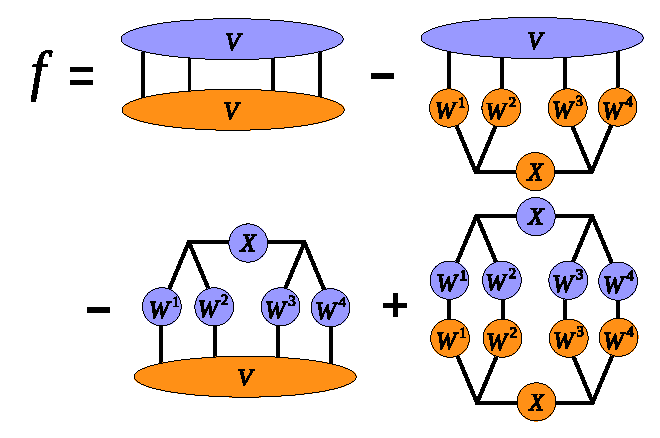
\includegraphics[width=0.5\textwidth]
{figures/tcc_theory/cost_function} } } .
\label{fig:cost_function}
\end{equation}
%
where we denoted conjugated tensors by darker color. Clearly, the best possible 
THC approximation to $V$ will correspond to a minimum of the cost function $f$. 
Since $f$ is a real-valued analytic function, its derivatives with respect to 
possibly complex factors $W \in \{W^1, W^2, W^3, W^4, X\}$ are related by
$\frac{\partial f}{\partial W} = (\frac{\partial f}{\partial W^{\ast}})^{\ast}$.

In order to minimize the cost function, we proceed with the
calculation of its gradient, which can be easily done using
diagram~\ref{fig:cost_function}.  The partial derivative of $f$ with
respect to $W^1$ is
%
\begin{equation}
\vcenter{
\hbox{
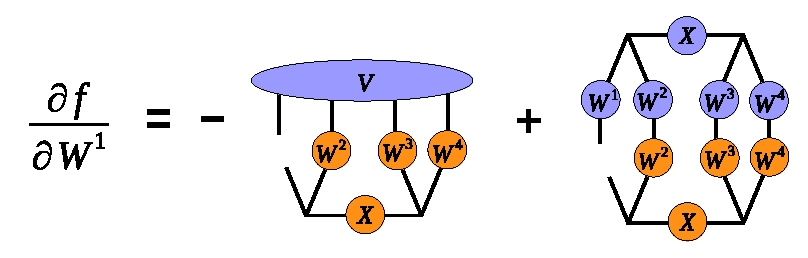
\includegraphics[width=0.7\textwidth]
{figures/tcc_theory/cost_function_dfdw1}}}
\label{fig:cost_function_partial}
\end{equation}
%
Likewise, partial derivatives of $f$ with respect to other factors are 
expressed by similar diagrams with those factors removed. Using the fact that 
$\frac{\partial f}{\partial W}$ is linear in $W^\ast$, we can contract all 
factors around $W^\ast$ into an environment matrix $A$, as shown in 
diagram~\ref{fig:least_squares_w1}, and set this derivative to zero:
%
\begin{equation}
\vcenter{\hbox{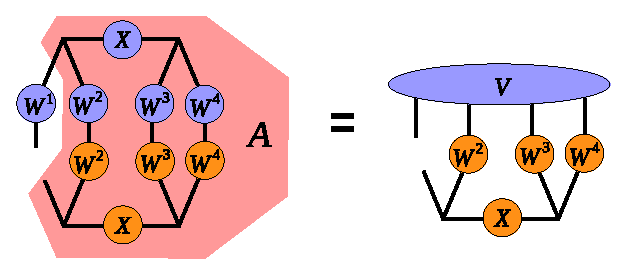
\includegraphics[width=0.5\textwidth]
{figures/tcc_theory/least_squares_w1} } }
\label{fig:least_squares_w1}
\end{equation}
%
We end up with a problem
%
\begin{equation}
A \cdot W^\ast = B.
\label{eq:least_squares_w1}
\end{equation}
%
The solution to Eqn.~\ref{eq:least_squares_w1} can be
obtained by multiplying from the left by the inverse of $A$ (or a 
pseudoinverse, if $A$ is a rank-deficient matrix).  Finally, we arrive to an 
expression for ${W^{1}}^{\ast}$, which diagrammatrically is
%
\begin{equation}
\vcenter{
\hbox{
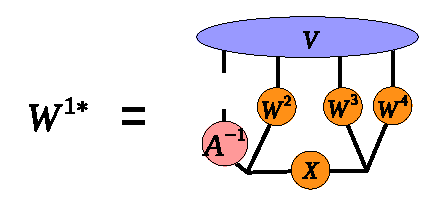
\includegraphics[width=0.4\textwidth]
{figures/tcc_theory/least_squares_w1_sol}}}
 .
\label{fig:least_squares_w1_sol}
\end{equation}
%
Let us estimate the cost of this procedure. We call the size of the 
auxiliary indices $\alpha, \alpha^{\prime}$ the rank of the THC 
decomposition ($r_\mathrm{THC}$). The construction of the environment 
matrix $A$ scales as $O(r_\mathrm{THC}^3)$, as does computing its generalized 
inverse. If each of the dimensions of $V$ equals $N$, then the cost of 
calculating ${W^1}^{\ast}$ scales as $O(N^4 \, r_\mathrm{THC})$. Updates for the
rest of the terms in the THC decomposition can be calculated similarly.

A simple iterative optimization algorithm can be built as follows.
First, the THC factors $W$ are initialized randomly.  For each factor,
an update is calculated as shown on diagram~\ref{fig:least_squares_w1_sol}, 
keeping the other factors fixed.  The process is iterated until convergence of 
the factors. We note that this procedure is, in fact, very similar to 
partial gradient descent and the Gauss-Siedel method.\cite{yoon1988lower} The 
resulting THC-ALS algorithm is listed below.
%
\begin{algorithm}[H]
  \caption{Alternating Least Squares}\label{code:thc_als}
  \begin{algorithmic}[1] 
  \Function{thc-als}{$V, r_\mathrm{THC}, \epsilon$}
  \State $I_{1},I_{2},I_{3},I_{4} \gets$ size($V$)
  \State $W^1, W^2, W^3, W^4, X \gets$ init\_random($I_{1}, I_{2}, I_{3}, 
I_{4}, r_\mathrm{THC}$) 
  \Repeat \ForAll {$W \in \{W^1, W^2, W^3, W^4,
X\}$}
  \State $A_{W} \gets $ get\_environment($W^1, W^2, W^3, W^4, X$)
  \LineComment{$O(r_\mathrm{THC}^3)$}
  \State $B_{W} \gets $ get\_rhs($V,
   W^1, W^2, W^3, W^4, X$) \LineComment{$O(N^4 \, r_\mathrm{THC})$ or
$O(N^2 \, r_\mathrm{RI} \, r_\mathrm{THC})$ with RI}
   \State $W_{new} \gets A^{-1} B$\Comment{$O(r_\mathrm{THC}^3)$}
   \EndFor
   \State $\Delta \gets \max_{W} \frac{\| W_{new} - W \|}{\|
W \|}$
   \State $W \gets W_{new}$ 
   \Until $\Delta > \epsilon$ 
   
   \Return $W^1, W^2, W^3, W^4, X$
    \EndFunction
  \end{algorithmic}
\end{algorithm}
%
The calculation of the right hand side of
Eqn.~\ref{eq:least_squares_w1} dominates in the cost of THC-ALS,
scaling as $O(N^4 \, r_\mathrm{THC})$. A simple modification is
possible to reduce the cost of this step by one order of magnitude. If an
RI approximation to the original tensor $V$ is available from the beginning, as 
in the case of the electron interaction, it can be used in place of $V$, 
leading to a faster algorithm. The diagram corresponding to 
Eqn.~\ref{eq:least_squares_w1} then becomes
%
\begin{equation}
\vcenter{\hbox{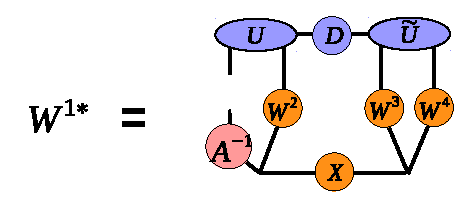
\includegraphics[width=0.4\textwidth]
{figures/tcc_theory/least_squares_w1_sol_ri} } }
\label{fig:least_squares_w1_sol_ri}
\end{equation}
%
The cost of the expression above scales as $O(N^2 \,
r_\mathrm{RI} \, r_\mathrm{THC})$, because the contraction of a
fourth-index tensor $V$ with matrices $W$ is replaced by contractions
of two third-index tensors $U$ and $\tilde{U}$. We only need to
modify the function $get\_rhs()$ in the Algorithm~\ref{code:thc_als} to build a 
lower scaling algorithm,
which we refer to as THC-ALS-RI.

Alternating least squares algorithms are simple and 
often robust,\cite{uschmajew2012local} but may take a large number of
iterations to converge.\cite{comon2009tensor} Particularly, we found that 
calculating THC decomposition with ALS directly is inferior to using a two 
step scheme mentioned earlier.\cite{schutski2017tensor} Nevertheless, the ALS 
procedure can be derived for various decompositions, and is a cornerstone of 
our tensor structured coupled cluster.

\section{Tensor Structured Coupled Cluster}
The ALS algorithm can be merged together with CC equations, leading to
CC expressions with significantly lower computational cost, which are the main 
achievement of our work.\cite{schutski2017tensor} The logic of deriving those 
novel approaches follows the same route as in the case of the ALS method. Here, 
we will use coupled cluster doubles (for which one neglects ${}^1\hat{T}$) as as 
example, and THC decomposition of all four index tensors. This scheme, 
however, is quite general, and we have applied it to other decompositions and 
coupled cluster methods, as discussed in subsequent sections. 

Let us impose the THC structure on the doubles amplitudes. We
approximate the amplitude tensor ${}^{2}T$ with its THC decomposition
${}^{2}\tilde{T}$ having rank $r_{T}$.  The difference between the original and 
approximated amplitudes is
%
\begin{equation} 
\Delta_{T} = {}^{2}T - {}^{2}\tilde{T} = {}^{2}T -
(Y^{2} \odot Y^{1}) \cdot Z \cdot (Y^{4} \odot Y^{3})^{T},
\end{equation}
%
where $Y^{i}$ and $Z$ are factor matrices in the THC
decomposition of ${}^{2}T$. As in the case of the ALS algorithm, we wish to 
minimize the squared norm of the error tensor $\Delta_{T}$, which is the 
minimization of 
the corresponding cost function $f_{T}$,
%
\begin{equation}
f_{T} = |\Delta_{T}|^2 = ({}^{2}T^{\ast} -
{}^{2}\tilde{T}^{\ast})({}^{2}T - {}^{2}\tilde{T}).
\end{equation}
%
Setting partial derivatives of $f_{T}$ with respect to
the decomposition factors to zero, we obtain a new set of equations
%
\begin{equation} 
\frac{\partial f_{T}}{\partial Y} = - {}^{2}T^{\ast}
\frac{\partial {}^{2} \tilde{T}}{\partial Y} + {}^{2}\tilde{T}^{\ast}
\frac{\partial {}^{2} \tilde{T}}{\partial Y} = 0,
\label{eq:cc_cost_function}
\end{equation}
%
where $Y \in \{Y^{1}, Y^{2}, Y^{3}, Y^{4}, Z\}$. Again,
as $f_{T}$ is real and analytic, only one set of derivatives (either
with respect to $Y$ or $Y^{\ast}$) is sufficient to find its minimum.

As we recall from Section~\ref{sec:preliminaries_rccd}, the amplitude equation 
in CCD method is:
\begin{equation}
{}^{2}T = {}^{2}G({}^{2}T) \cdot {}^{2}D, 
\label{eq:ccd_amplitude_equation_tcc}
\end{equation}

We proceed by replacing ${}^2T^\ast$ in Eqn.~\ref{eq:cc_cost_function} with 
the right hand side of Eqn.~\ref{eq:ccd_amplitude_equation_tcc}. 
Effectively, this corresponds to minimizing the difference between a decomposed 
tensor ${}^2\tilde{T}$ and a solution of the CCD amplitude equations. The 
resulting amplitude equations are:
%
\begin{equation}
\tilde{T}^{\ast} \frac{\partial \tilde{T}}{\partial
Y} = {}^{2}G \cdot {}^{2}D \cdot \frac{\partial \tilde{T}}{\partial Y}.
\end{equation}
%
This is the analogue of Eqn.~\ref{eq:least_squares_w1}
in THC-ALS, and can be solved with the help of the pseudoinverse as the 
left-hand-side is linear in $Y^\ast$.  Diagrammatically, we have
%
\begin{equation}
\vcenter{\hbox{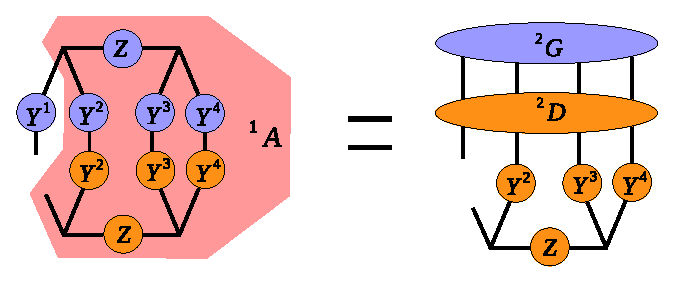
\includegraphics[width=0.6\textwidth]{figures/tcc_theory/cc_thc}}
} .
\label{fig:cc_thc}
\end{equation}
%
Note that the energy denominator ${}^2D$ is represented 
here as an order-8 diagonal tensor ${}^2D^{aba^{\prime} b^{\prime}}_{ij 
i^{\prime} j^{\prime}}$, instead of an order-4 dense tensor ${}^2D^{ab}_{ij}$ 
as in Eqn.~\ref{eq:cc_denom_definition}. The final form of our ALS-type 
coupled cluster doubles equations is provided below (an example for the factor 
$Y^{1}$ is shown; expressions for other factors are analogous):
%
\begin{equation}
\vcenter{\hbox{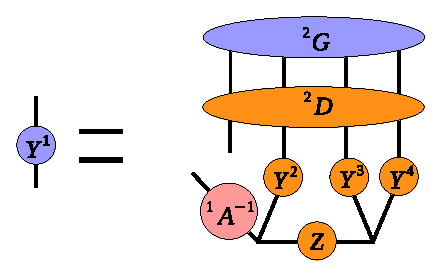
\includegraphics[width=0.4\textwidth]
{figures/tcc_theory/cc_thc_sol}}}.
\label{fig:cc_thc_als}
\end{equation}
%

Here ${}^2G$ on the right hand side is a collection of tensor contractions 
involving the Hamiltonian and THC approximated ${}^2T$ amplitudes 
(see Eqn.~\ref{eq:ccd_amplitude_equation} for the full list of these terms).
We substitute the electron interaction term with its THC decomposition 
calculated beforehand, for example, with ALS. The size of the auxiliary 
dimension in this decomposition is $r_{V}$, and needs to be only of order $O(N)$ 
for a good approximation, as was discussed previously in the section 
\ref{sec:tensor_hypercontraction}. We also substitute the denominator tensor by 
its CP decomposition obtained analytically by means of Laplace transformation. 
The CP rank $r_{D}$ in this decomposition is a small constant $\sim 15$ and 
does not depend on $N$. Finally, we \emph{define} ${}^2T$ amplitudes to have 
THC structure with rank $r_{T}$. The resulting expressions, where all order-4 
tensors are substituted by their decompositions, factorize. After defining 
proper intermediates, the cost of these equations has quartic scaling in 
$r_{V}$, $r_{T}$ and $N$ per iteration. An example of such factorization 
for the contraction we considered before 
in Eqn.~\ref{eq:ccd_intermediate_example2} is 
shown below diagrammatically (we used a dashed line to show an auxiliary 
index in the CP decomposition of ${}^2 D$):
\begin{equation}
\begin{split}
\tau^{ab}_{ij} & = {}^2 T^{cd}_{ij} V^{ab}_{cd} \\
Y^{1 \ast} &\longleftarrow {}^1A^{-1} \cdot \tau \cdot {}^{2}D 
\cdot \frac{\partial ({}^2\tilde{T})}{\partial Y^{1}}
\end{split}
\end{equation}
%
\begin{equation}
\vcenter{\hbox{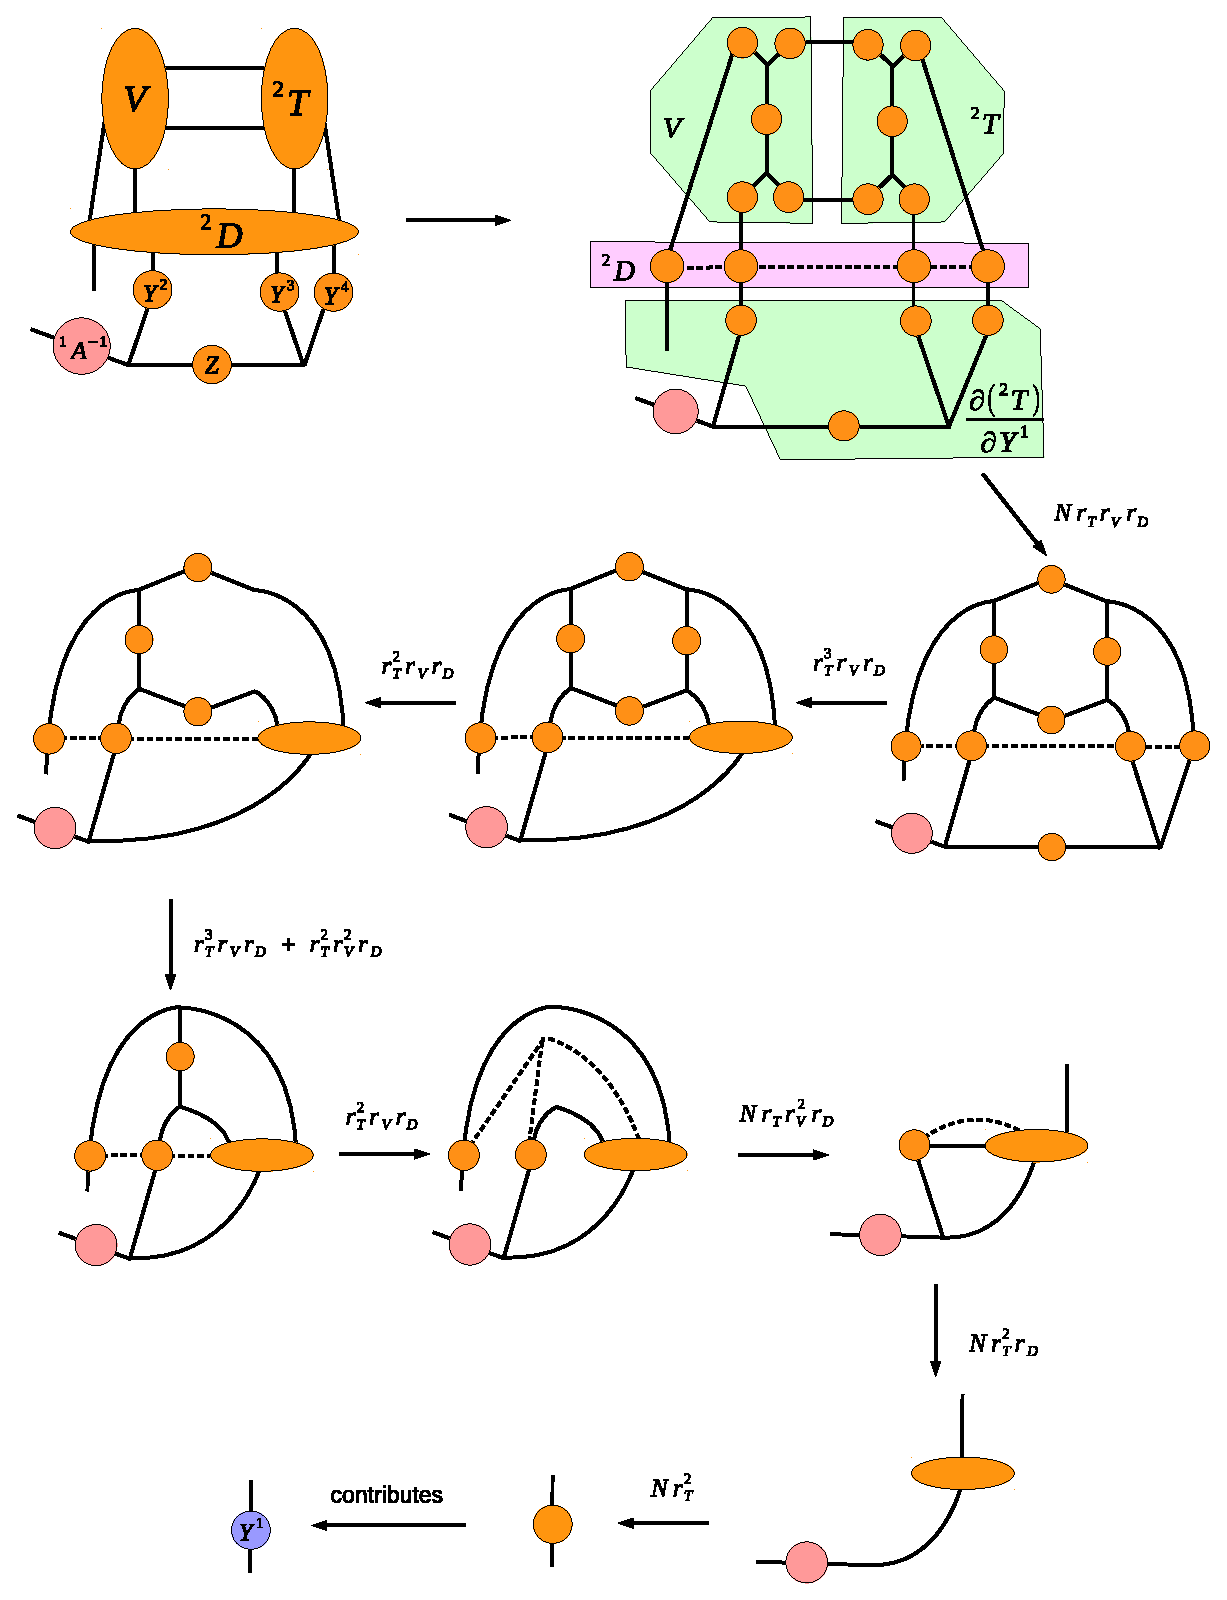
\includegraphics[width=0.95\textwidth]
{figures/tcc_theory/cc_thc_example}}}.
\label{fig:cc_thc_example}
\end{equation}
%
Although diagrams are convenient for explaining tensor factorizations, it 
is still quite challenging to define good intermediates even for the 
simplest decomposed RCCD method. We derived factorized equations using an 
automated algebraic system developed in our group.\cite{drudge1, drudge2} We 
refer the reader to the supplementary material from 
Ref.~\cite{schutski2017tensor} for the complete listing of these expressions for 
the THC decomposed RCCSD method (denoted as THC-RCCSD), as well as their 
implementation in Python.\cite{van2007python}

The algorithm of tensor structured coupled cluster is listed below. 
%
\begin{algorithm}[H]
  \caption{Tensor Structured Coupled Cluster}\label{code:tcc_algorithm}
  \begin{algorithmic}[1] 
  \Function{thc}{$H, r_\mathrm{V}, r_\mathrm{T}, \epsilon_{T}, \epsilon_{E}$}
  \State $F, W^{1},W^{2},\ldots \gets$ approximate\_hamiltonian($H, r_{V}$)
  \State ${}^2D^1,{}^2D^{2},\ldots \gets$ 
Laplace\_transform\_denominator($F$)  
  \State $\tilde{Y}^1, \tilde{Y}^2, \tilde{Y}^3 \ldots \gets$ 
init\_random\_amplitude\_decomposition($r_{T}$) 
  \Repeat 
  \State $Y^1, Y^2, Y^3, \ldots \gets 
$ symmetrize\_amplitudes($\tilde{Y}^{1}, \tilde{Y}^{2}, \tilde{Y}^{3} \ldots$)
   \State $E \gets $ calculate\_cc\_energy($F, W^1, W^2, \ldots, 
\tilde{Y}^{1}, \tilde{Y}^{2}, \ldots$)
  \ForAll {$Y \in \{\tilde{Y}^{1}, \tilde{Y}^{2}, \tilde{Y}^{3}, 
\ldots \}$}
  \State $A_{Y} \gets $ get\_environment($Y^1, Y^2, Y^3, \ldots \tilde{Y}^1, 
\tilde{Y}^2, \tilde{Y}^3, \ldots$)
  \State $B_{Y} \gets $ get\_cc\_rhs($F, W^1, W^2, \ldots, {}^2D^{1}, 
{}^2D^{2}, \ldots Y^{1}, Y^{2}, Y^{3}, \ldots \tilde{Y}^{1}, \tilde{Y}^{2}, 
\ldots$) 
   \State $\tilde{Y}_{new} \gets A^{-1} B$
   \EndFor
   \State $\Delta \gets \max_{Y} \frac{\| \tilde{Y}_{new} - \tilde{Y} \|}{\|
\tilde{Y} \|}$
   \State $\tilde{Y} \gets \tilde{Y}_{new}$ 
   \State $E_{new} \gets $ calculate\_cc\_energy($F, W^1, W^2, \ldots, 
\tilde{Y}^{1}, \tilde{Y}^{2}, \ldots$)
   \State $dE \gets E - E_{new}$
   \Until $\Delta > \epsilon_{T}$ or $dE > \epsilon_{E}$ 
   
   \Return $E, \tilde{Y}^1, \tilde{Y}^2, \tilde{Y}^3, \ldots$
    \EndFunction
  \end{algorithmic}
\end{algorithm}
%
Let us walk though the algorithm. First, a 
decomposition of the two body interaction and the Laplace transformation of 
energy denominators are calculated. Next, the factors in the decomposition of 
amplitudes are initialized with random numbers. For each factor in the 
decomposition of amplitudes its environment and the right hand side in the 
ALS-like equation are calculated (see Eqn.~\ref{fig:cc_thc}). The factors  are 
updated according to Eqn.~\ref{fig:cc_thc_als} until convergence in either the 
coupled cluster energy or the elements of factors is reached.

An important detail of the algorithm is that proper symmetries have to be 
enforced by the decomposition of amplitudes in order for 
the method to converge (See Appendix~\ref{sec:symmetrization} for more 
details). Symmetrization of the decomposition of amplitudes, however, causes 
the growth of decomposition rank $r_{T}$, the situation we would like 
to avoid. This can be done by keeping two sets of amplitudes at each 
iteration. Here we denoted symmetrized factors by $Y$, and their 
unsymmetrized counterparts as $\tilde{Y}$. We used symmetrized factors to 
evaluate ${}^2G({}^2 \tilde{T})$ (see Eqn.~\ref{fig:cc_thc}, dark colored 
shapes), while unsymmetrized factors were used to project ${}^2G({}^2 
\tilde{T}) \cdot {}^2D$ in the ALS-like manner (Eqn~\ref{fig:cc_thc}, light 
colored shapes). This scheme allowed us to keep the rank 
$r_{T}$ fixed from iteration to iteration, while preserving proper symmetries of 
the amplitude tensors, which is required in coupled cluster theory. 

To summarize, equation~\ref{fig:cc_thc_als}, which represents a combination 
of CC and ALS update, is a cornerstone of the tensor structured coupled cluster 
method and the main achievement of this work. Our scheme is quite generic  
and can be applied to any combination of the factorizations of amplitudes and 
the Hamiltonian. In the following sections we will discuss numerical experiments 
with some of those novel methods.


\section{Appendix
\label{sec:Appendix}}
\subsection{Graphical notation
\label{sec:graphical_notation}}
We have extensively used wiring diagrams to represent complicated contractions 
of tensor expressions though the text. This notation is similar to the standard 
diagrams in many-body physics,\cite{mattuck2012guide} but is simpler. We use 
this notation mainly to evaluate the complexity of operations, and also to 
simplify the search for intermediates in complicated expressions.  

In our notations, tensors are represented by shapes.  Typically a
$d$-order tensor is depicted by a polygon with $d$ corners (and a
second-order tensor by a circle), though we have not followed this
convention universally. Indices are denoted by lines; a line
connecting multiple tensors is to be summed over, and open lines
correspond to free indices. If a particular element of a tensor
expression is required, we label the open lines.

As an example, a matrix product would be represented by
%
\begin{equation}
\vcenter{\hbox{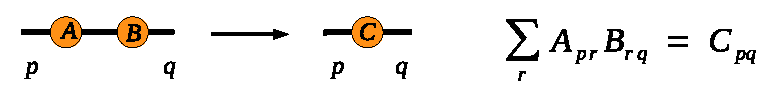
\includegraphics[width=0.7\textwidth]
{figures/tcc_theory/simple_diagrams11}}
}
\end{equation}
%
and a more general contraction of a fourth-order tensor
with a third-order tensor can be shown as
%
\begin{equation}
\vcenter{\hbox{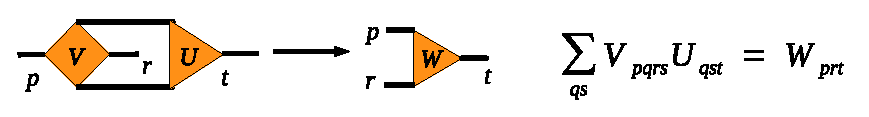
\includegraphics[width=0.7\textwidth]
{figures/tcc_theory/simple_diagrams12}}} .
\end{equation}
%
Diagrams can be used to readily estimate the cost of contractions and
other operations.  The cost $\Omega$ of contracting two tensors over
$L$ indices of size $\{ \lambda \}_1^{L}$ to a tensor with $M$ indices
of size $\{ \mu \}_1^M$ scales with respect to $N$ as
%
\begin{equation} 
\Omega = \mathcal{O}(N^{\sum_{l = 1}^{L} log_{N}
\dim(\{\lambda\}_l) \cdot \sum_{m = 1}^M log_{N} \dim(\{\mu\}_m)}).
\label{eq:contract_scaling_estimate}
\end{equation} 
%
Put simply, the cost of a contraction will scale as $N$ taken to the power of 
the sum of the number of contracted lines and the number of open lines.  
For example, a contraction of two third-order tensors of size $N \times N 
\times N$ over two indices of size $N$ scales as $O(N^4)$:
%
\begin{equation}
\vcenter{\hbox{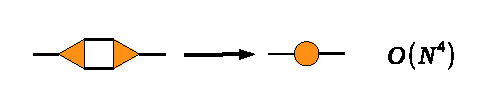
\includegraphics[width=0.6\textwidth]
{figures/tcc_theory/simple_diagrams2}}}
\label{fig:contraction_scaling}
\end{equation}
%
Other operations one may wish to perform on tensors are of outer product type. 
An outer product can be viewed as a contraction over an additional index of 
size one. Diagrammatically, outer products correspond to 
merging the nodes together and leaving all lines in the final structure:
%
\begin{equation}
\vcenter{\hbox{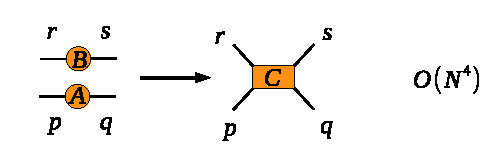
\includegraphics[width=0.5\textwidth]
{figures/tcc_theory/simple_diagrams3}}}
\label{fig:outer_product}
\end{equation} 
%
Note that if one reshapes the fourth-order tensor above
into a matrix with combined indices $rp$ and $sq$, then the result
will coincide with the usual Kronecker product of matrices, where we
recall that the Kronecker product is
%
\begin{equation}
C = A \otimes B \Leftrightarrow C_{rp, sq} = A_{p,q}
\cdot B_{r,s}.
\end{equation}
%
The cost of outer product-type operations is
%
\begin{equation}
\Omega = \mathcal{O}(N^{\sum_{m = 1}^{M} log_{N}
dim(\{\mu\}_m)})
\label{eq:outer_scaling_estimate}
\end{equation}
%
where $\{ \mu \}_1^{M}$ are $M$ free indices in the
resulting tensor.

For our purposes we slightly extended the diagrammatic notation by
introducing summations over an index shared by more than two terms. We
denote such indices by branching lines with a dot at the branching
point. This dot can be interpreted either as an index of the summation
itself, or as a fully diagonal tensor whose elements are contractions
of Kronecker deltas, e.g.
%
\begin{equation} K_{p,q,r,\ldots} = \sum_\alpha \delta_p^\alpha
\delta_q^\alpha \delta_r^\alpha \ldots.
\end{equation}
%
The latter interpretation means that all contractions
in the diagrams can be thought pairwise as in the normal case.
A similar extension has been proposed before in the tensor network 
literature.\cite{ying2016tensor} Using our new
notation, contracting a canonical polyadic decomposition of a third
order-tensor back to a full tensor can be represented as
%
\begin{equation}
\vcenter{\hbox{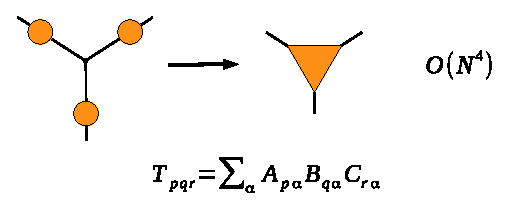
\includegraphics[width=0.5\textwidth]
{figures/tcc_theory/simple_diagrams4}}}
\label{fig:dot_in_diagrams}
\end{equation}
%
If the dimensions of this tensor are $N \times N \times
N$ and the rank of the decomposition (the dimension of the auxiliary
index $\alpha$) is $N$, then the cost of rebuilding the original
tensor from its decomposed form will scale as $O(N^4)$. We note that
Eqn.~\eqref{eq:contract_scaling_estimate} holds in this case just the
same way as with normal pairwise contractions.

Virtually all matrix operations can be seen as either inner or outer 
product, or a combination of them. Let us also provide diagrammatic  
representations of some frequent operations. The Frobenius 
norm of a tensor, which we recall is
%
\begin{equation} \| A \| = \sqrt{\sum_{pqrs \ldots}
A_{pqrs\ldots} \, A^\ast_{pqrs\ldots}},
\end{equation}
%
is given diagrammatically as the square root of a
tensor fully contracted with its own conjugate:
%
\begin{equation}
\vcenter{\hbox{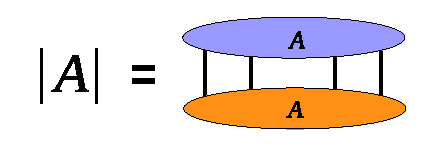
\includegraphics[width=0.3\textwidth]
{figures/tcc_theory/frobenius_norm}}}.
\label{fig:frobenius_norm}
\end{equation}
%
A darker color is used here (as well as in the text) to denote complex
conjugation.

The column-wise Khatri-Rao product is represented by
%
\begin{equation}
D = A \odot B ~~\Leftrightarrow ~~D_{qp,\alpha} =
A_{p,\alpha} \cdot B_{q,\alpha}.
\end{equation}
%
Note that $A$ and $B$ should have the same number of
columns to be compatible. The Khatri-Rao product can be understood as a partial 
outer product over the row indices, while column indices are simply matched. 
The resulting matrix $D$ can be reshaped to a third-order tensor with indices 
$p$, $q$ and $\alpha$. Diagrammatically, the Khatri-Rao product is
%
\begin{equation}
\vcenter{\hbox{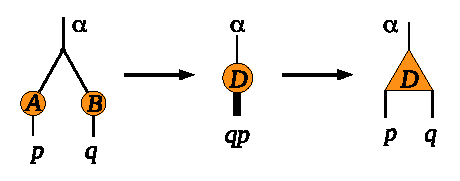
\includegraphics[width=0.5\textwidth]
{figures/tcc_theory/simple_diagrams5}}}.
\label{fig:khatri_rao_product}
\end{equation} 
%
Here we used a thick line to denote a combined index
$qp$. Note also that the canonical polyadic decomposition can be
conveniently expressed through the Khatri-Rao product, which is also
reflected by the diagrams:
%
\begin{equation}
\vcenter{\hbox{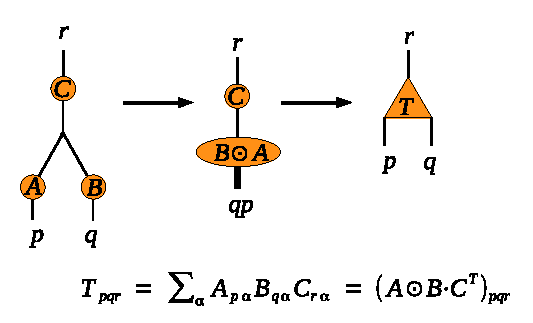
\includegraphics[width=0.6\textwidth]
{figures/tcc_theory/simple_diagrams7}}}
\label{fig:canonical_khatri_rao}
\end{equation}
%
Finally, we point out that wiring diagrams provide an easy way to
calculate derivatives.  A partial derivative of a tensor network with
respect to one of its component tensors is simply the network with
that tensor (but not its lines) removed. On the Figure~\ref{fig:deriv_example}
the derivative of a tensor $T_{ijk} = \sum_{p} A_{ip} B_{jp} C_{kp}$ with 
respect 
to the matrix $A_{mn}$ is shown. We note that one can insert an identity matrix 
$I$ into any edge of a tensor network as this does not alter the result of 
contractions, and also that a disjoint network can be interpreted as a 
Kronecker product of its parts.
%
\begin{equation}
\vcenter{\hbox{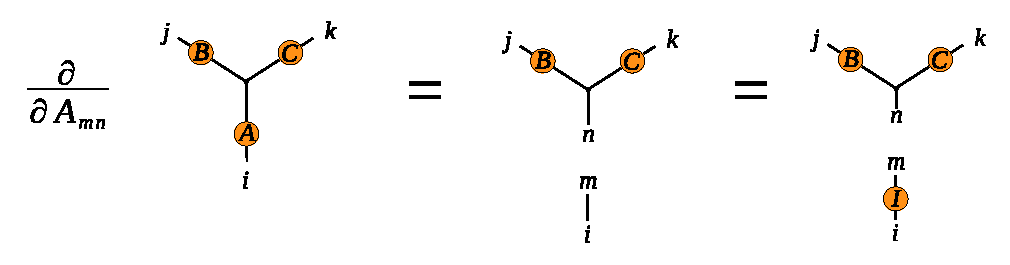
\includegraphics[width=0.9\textwidth]
{figures/tcc_theory/deriv_example}}}
\label{fig:deriv_example}
\end{equation}
%
By making use of the introduced matrix operations one can conclude that 
%
\begin{equation}
 \frac{\partial T}{\partial A} = (B \odot C) \otimes I
\end{equation}
%

\subsection{Symmetrization of tensor decompositions
\label{sec:symmetrization}}
Most of the tensors we used are coefficients of operators, and have to be 
(anti)symmetric with respect to index permutations required by their 
operator algebra. For an arbitrary tensor $\tilde{T}$ its symmetric 
part $T$ can be extracted with the help of the symmetrization operator. 
Lets suppose that $T$ is equivalent under a permutation of indices 
$\{\sigma_{\pi}\}_{\pi=1}^{\Pi}$. The symmetric part of $\tilde{T}$ can then be 
extracted as:
%
\begin{equation}
T_{ijk\ldots} = \frac{1}{\Pi} \sum_{\pi=1}^{\Pi} 
\tilde{T}_{\sigma_{\pi}(i) \sigma_{\pi}(j) \sigma_{\pi}(k) \ldots}
\end{equation}
%
As an example, the double excitation amplitudes in 
RCCD have the following symmetry:
\begin{equation}
 T_{ij}^{ab} = T_{ji}^{ba}
\end{equation}
The double excitation tensor can be symmetrized with the following operation:
%
\begin{equation}
 T_{ij}^{ab} = \frac{1}{2} (\tilde{T}_{ij}^{ab} + \tilde{T}_{ji}^{ba})
 \label{eq:symmetrization}
\end{equation}
%
Preserving proper symmetries of tensors is crucial in many-body methods. 
In the particular case of coupled cluster the violation of the symmetry of 
excitation amplitudes due to numerical noise may quickly lead to divergence of 
the otherwise convergent algorithm (see Figure~\ref{fig:symmetry_convergence}).
%
\begin{figure}[!ht]
\centering
\begin{subfigure}[b]{0.70\textwidth}
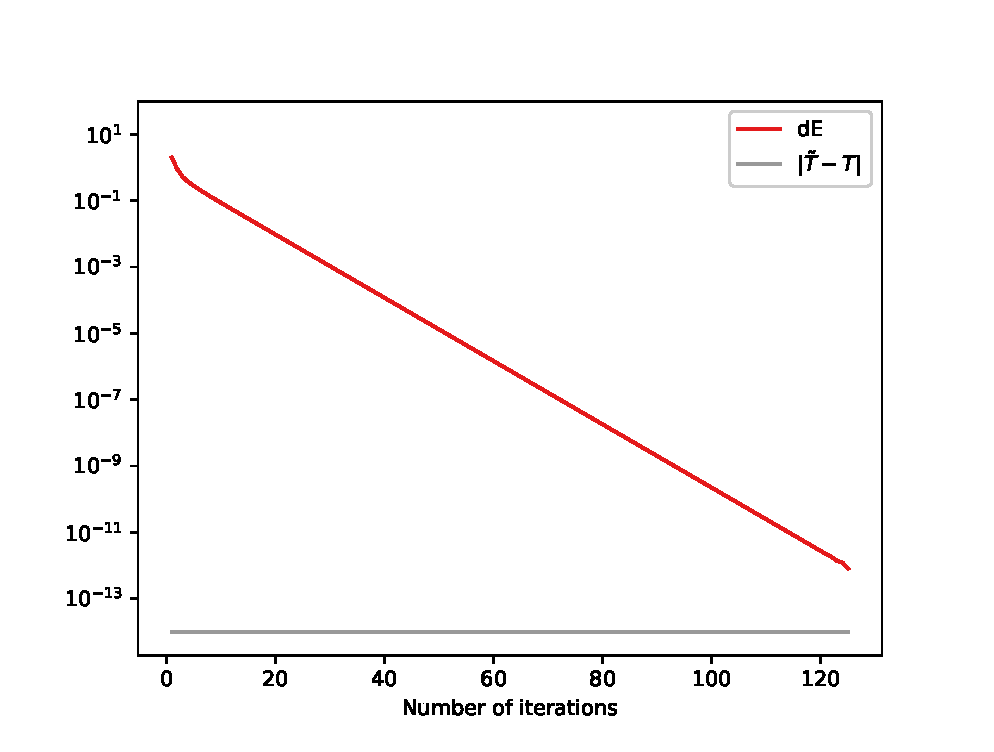
\includegraphics[width=1\linewidth]{figures/tcc_theory/dE_vs_niter_u_3_stable}
   \caption{}
   \label{fig:symmetry_convergence_1} 
\end{subfigure}
\begin{subfigure}[b]{0.70\textwidth}
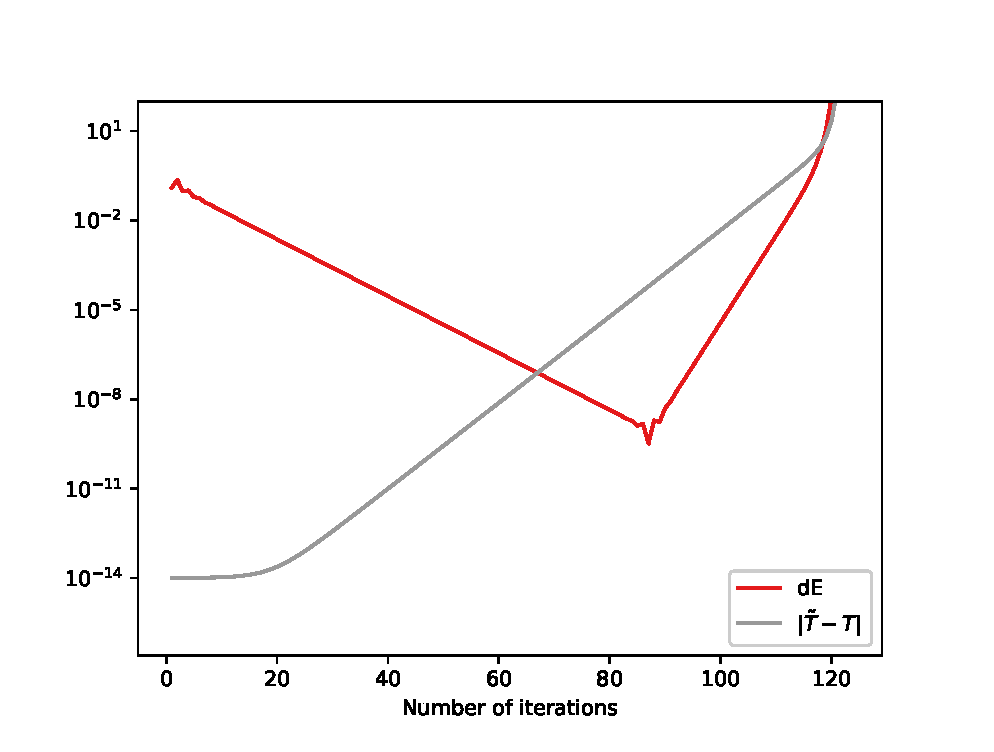
\includegraphics[width=1\linewidth]{figures/tcc_theory/dE_vs_niter_u_3_unst}
   \caption{}
   \label{fig:symmetry_convergence_2}
\end{subfigure}
\caption{Convergence of the RCCD method with (a) and without (b) enforcing the 
symmetry of ${}^2 T$ amplitudes. The lower panel shows the divergence of RCCD 
iterations due to the accumulation of numerical noise, while the same algorithm 
converges to machine precision if the noise is eliminated.}
\label{fig:symmetry_convergence}
\end{figure}
%
Decompositions of higher order tensors, however, are usually not constrained 
to strictly preserve permutation symmetries. It is important though to provide 
a way of symmetrizing tensor decompositions \emph{directly} (e.g. without 
rebuilding high order tensors, as this will eliminate all benefits of the 
decomposition).

\subsubsection{Canonical decomposition}
Canonical decomposition can be symmetrized by using its summation and 
permutation properties.
\begin{itemize}
  \item For a tensor $T$ having a canonical decomposition $T_{ijk} = \sum_{p} 
A_{ip} B_{ip} C_{jp}$ its permutations can be built by simply permuting the 
order of factors in the summation.
  \item If tensors $T$ and $U$ both have canonical decompositions with ranks 
$r_{T}$ and $r_{U}$ respectively, then their sum is a canonical decomposition 
with rank $r = r_{T} + r_{U}$. This means that the factor matrices of $T$ and 
$U$ can be concatenated column-wise:
%
\begin{equation}
\begin{aligned}
 T_{ijk} &= \sum_{p=1}^{r_{T}} A_{ip} B_{jp} C_{kp}, \qquad U_{ijk} = 
\sum_{p=1}^{r_{U}} D_{ip} E_{jp} F_{kp} \\
(T + U)_{ijk} &= \sum_{p=1}^{r_{T} + r_{U}} (A | D)_{ip} (B | E)_{jp} (C | 
F)_{kp}
\end{aligned}
\end{equation}
where we used $(A | D)$ to denote a column-wise concatenation of matrices $A$ 
and $D$
\end{itemize}
 
Using the properties of the CPD it is possible to symmetrize tensors directly 
in their decomposed form. Suppose that an amplitude tensor has a 
canonical decomposition:
%
\begin{equation}
 \tilde{T}_{ij}^{ab} = \sum_{p=1}^{P} W^{1}_{ap} W^{2}_{bp} 
W^{3}_{ip} W^{4}_{jp}
\end{equation}
%
Then the symmetric part of $T$ can be 
represented as:
%
\begin{equation}
\begin{aligned}
 T_{ij}^{ab} &= \frac{1}{2} (\tilde{T}_{ij}^{ab} + \tilde{T}_{ji}^{ba}) \\
 T_{ij}^{ab} &= \frac{1}{2} \sum_{p=1}^{2P} (W^{1} | W^{2})_{ap} (W^{2} | 
W^{1})_{bp} (W^{3} | W^{4})_{ip} (W^{4} | W^{3})_{jp} 
\end{aligned}
\end{equation}
%
the normalization scalar can be absorbed into one of the new factors. We note 
that the symmetrized decomposition may not have an optimal rank (e.g. 
CPD with a lower rank and same accuracy may exist), but this growth of rank did 
not pose a problem in our applications.

\subsubsection{Tensor Hypercontraction}
The symmetrization expressions in case of THC factorization can be build 
using an analogous reasoning. If a tensor $\tilde{T}$ has a 
THC decomposition $\tilde{T}_{ij}^{ab} = \sum_{pq} W^{1}_{ap} W^{2}_{ip} X_{pq} 
W^{3}_{bq} W^{4}_{jq}$, then it can also be regarded having a CP decomposition 
with a "thick" factor $Q_{R}$, as is shown below:
%
\begin{equation}
\vcenter{\hbox{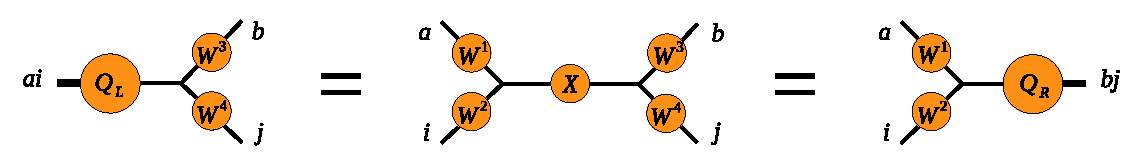
\includegraphics[width=0.9\textwidth]
{figures/tcc_theory/thc_as_cpd_sym}}}.
\label{fig:thc_as_cpd_sym}
\end{equation}
%
The same is true for the left part of the THC tensor network. The final 
result of the symmetrization is:
%
\begin{equation}
\begin{aligned}
 T_{ij}^{ab} &= \frac{1}{2} (\tilde{T}_{ij}^{ab} + \tilde{T}_{ji}^{ba}) \\
 T_{ij}^{ab} &= \frac{1}{2} \sum_{p=1}^{2P}\sum_{q=1}^{2Q} (W^{1}|W^{3})_{ap} 
(W^{2}|W^{4})_{ip} \left(
\begin{array}{c|c}
X & 0 \\
\hline
0 & X^{T}
\end{array}
\right)_{pq} (W^{3}|W^{1})_{bq} (W^{4}|W^{2})_{jq}  
\end{aligned}
\label{eq:thc_symmetrization}
\end{equation}
%
As one may notice from Eqn.~\ref{eq:thc_symmetrization}, the number 
of elements in the factor $X$ grows as a square of the number of symmetry 
operations. This happens because the symmetry $T_{ij}^{ab} = T_{ji}^{ba}$ 
permutes pairs of indices ($ai$ and $jb$) located farther away from each other 
compared to CPD. It follows again that the structure of the decomposition plays 
a crucial role in what tensors the decomposition can effectively approximate.

\chapter{Applications of Tensor Structured Coupled Cluster
\label{ch:app_tcc}}
In this chapter we will present results for our tensor structured CC approach. 
We introduce present two approximate CC methods based on different tensor 
factorizations. Section~\ref{sec:thc_rccsd} discusses what we call THC-RCCSD, 
and was the subject of Ref.~\cite{schutski2017tensor}. 
Section~\ref{sec:cpd_rccsd} discusses a newer development we call CPD-RCCSD. 
Finally, the Section~\ref{sec:strong_correlation} shows how tensor structured 
coupled cluster can be used to remedy deficiencies of CC for strongly correlated 
problems.

\section{THC-RCCSD method
\label{sec:thc_rccsd}}
\subsection{Introduction}
In this section we present the first application of our tensor structured 
coupled cluster theory. We start with the RCCSD method, where both the two body 
interaction part of the Hamiltonian and the ${}^2T$ amplitudes have THC 
structure. Note that ${}^2T$ is never built as a four index tensor, but is 
rather optimized in a decomposed form. This combination of decompositions 
results in a procedure with quartic cost in the basis size $N$ and the ranks of 
THC approximation. Diagrammatically, our choice of decompositions in THC-RCCSD 
can be summarized as:
%
\begin{equation}
\vcenter{\hbox{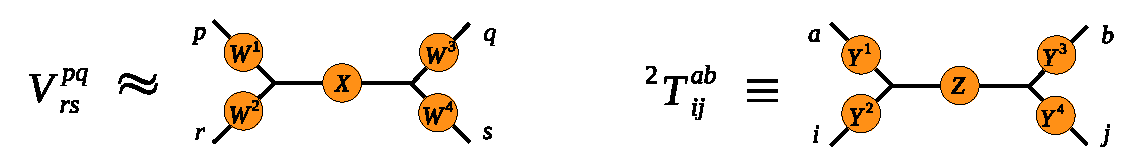
\includegraphics[width=0.9\textwidth]
{figures/thc_rccsd/rccsd_thc_def}}}
.
\label{fig:rccsd_thc_def}
\end{equation}
%
The index-based form of these decompositions is:
\begin{equation}
\begin{aligned}
 V^{pq}_{rs} \approx \sum_{\alpha, \beta} W^{1}_{p \alpha} W^{2}_{r \alpha} 
X_{\alpha \beta} W^{3}_{q \beta} W^{4}_{s \beta} \\
 {}^2T^{ab}_{ij} \stackrel{def}{=} \sum_{\mu \nu} Y^{1}_{a \mu} Y^{2}_{i 
\mu} Z_{\mu \nu} W^{3}_{b \nu} W^{4}_{j \nu}
\end{aligned}
\end{equation}

As both forms show, the two-electron interaction is decomposed in Mulliken 
order, as well as the two-body excitation amplitudes. To study the 
properties of THC-RCCSD we calculated energies of a set of small to medium size 
molecules.

\subsection{Computational details}
In our setup the decomposition of the electron interaction tensor was 
calculated with a two step method, as described in 
Ref.~\cite{schutski2017tensor} First, a partial singular value decomposition of 
the integrals in AO basis was calculated. We retained $r_{V}$ singular values 
and vectors. For larger systems, listed in Tab.~\ref{tab:energies_thc_rccsd}, 
RI-decomposed two-electron integrals were used in place of singular 
vectors. Next, a CP decomposition of rank $r_{V}$ of the resulting 
left and right singular vectors (arranged as three index tensors of size $N 
\times N \times r_{V}$) was calculated with ALS. The iterative least squares 
procedure was stopped when the ratio of the objective function $f$ to the 
square of the Frobenius norm of the original tensor dropped below $10^{-14}$, or 
a limit of 1000 iterations was reached.

In the subsequent coupled cluster calculations we chose the rank of the THC 
decomposition of ${}^2T$ amplitudes ($r_{T}$) to be equal to the rank 
used in approximating integrals, e.g. $r_{T} = r_{V}$. 
The CC iterations were stopped either after the energy was converged to within 
$10^{-9}$ Hartree or a limit of 250 iterations 
was reached. All calculations used the cc-pVDZ basis from the EMSL
database,\cite{schuchardt2007basis} and the corresponding cc-pVDZ-RI
was used in the RI approximation. The threshold for pseudoinverses was set to 
$10^{-10}$.

Our code was written in MATLAB and used Gaussian software~\cite{gaussian} 
for the calculation of two-electron integrals and Hartree Fock solutions. We 
also used Tensorlab~\cite{vervliettensorlab} to calculate CPD in the 
decomposition of two-electron integrals.

\subsection{Accuracy of THC for two electron integral approximation}
The accuracy of the THC decomposition of the two-electron integrals governs the
accuracy of the subsequent calculations. Thus, it is important to 
check the dependence of the error in the decomposition of
two-electron integrals on THC rank. Figure~\ref{fig:thc_err_mo_3systems} 
shows this error in a double logarithmic scale for three small molecules. 
Once again, we note that the decomposition is computationally useful if the 
rank $r_\mathrm{V}$ is close to the number of basis functions $N$.  As the 
figure shows, the error in the two-electron integrals decreases exponentially 
with respect to THC rank. We found that this trend holds for every system
tested. Further, there is no significant difference whether the two-electron 
integrals are decomposed in the atomic orbital or molecular orbital basis. As 
is demonstrated in Figure~\ref{fig:thc_err_ao_vs_mo}, the accuracy of the 
decomposition depends only slightly on the choice of the basis, and the ratio 
of errors in different bases is close to one.
%
\begin{figure}[tb]
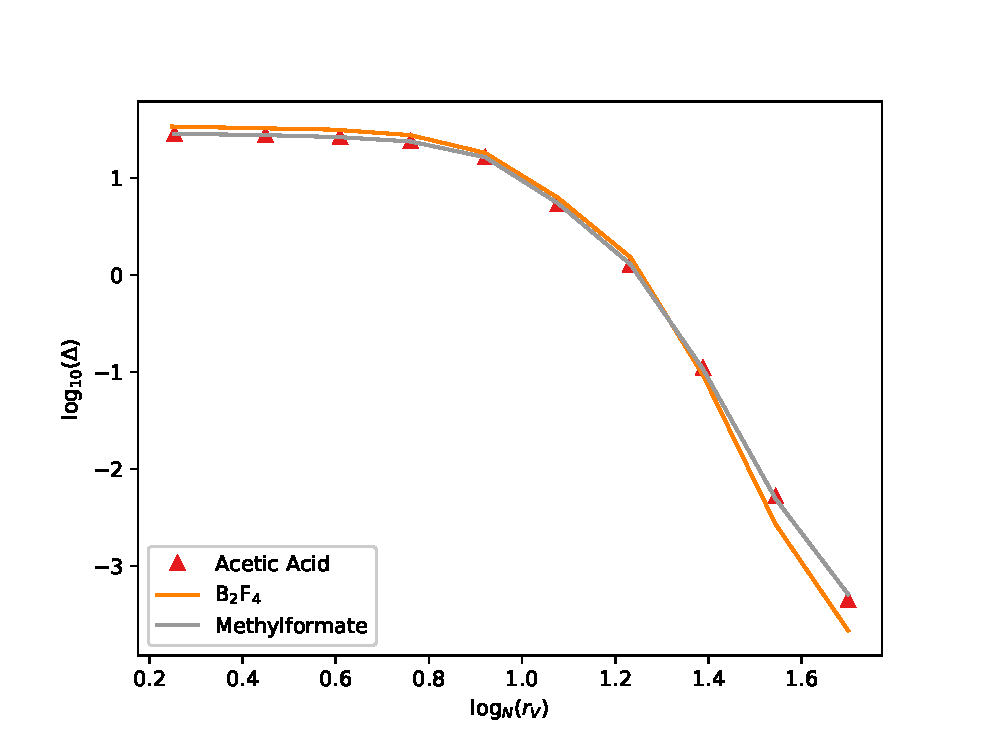
\includegraphics[width=\columnwidth]{figures/thc_rccsd/thc_err_mo_3systems}
\caption{Frobenius norm of error in THC decomposed two-electron integrals in 
atomic orbital basis as the function of rank $r_{V}$
\label{fig:thc_err_mo_3systems}}
\end{figure}
%
\begin{figure}[tb]
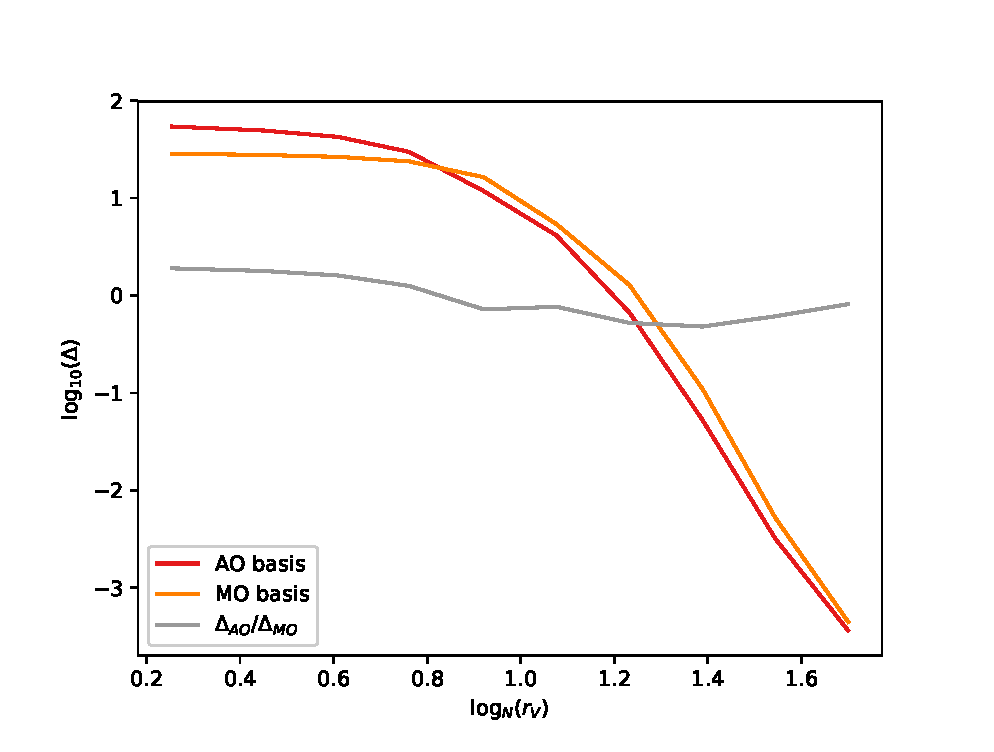
\includegraphics[width=\columnwidth]{figures/thc_rccsd/thc_err_ao_vs_mo}
\caption{Frobenius norm of error in THC decomposed two-electron integrals of 
Acetic Acid in atomic orbital and molecular orbital bases as the function of 
rank $r_{V}$
\label{fig:thc_err_ao_vs_mo}}
\end{figure}
%
To see how the errors in approximation of two-electron 
integrals influence the accuracy of subsequent energies, we checked 
the differences in the second-order M{\o}ller-Plesset (MP2) correlation
energy with respect to the exact MP2 calculation, as shown in 
Fig.~\ref{fig:mp2_err_ao_full}.  The combination
of MP2 and THC was first proposed by Hohenstein \emph{et
al}.\cite{hohenstein_thc2}; the computational effort of the method scales 
as $O(N^4)$.  The way these authors were calculating THC decomposition, however, 
was quite different from ours. As we found, the error in the MP2 correlation 
energy follows the trend seen in the decomposition of the integrals (see 
Fig.~\ref{fig:mp2_err_ao_full}). Results within $0.1~\mathrm{mH}$
of the exact value are already achieved with
$r_\mathrm{V} \sim N^{1.2} - N^{1.4}$.
We expect that the THC would work even better for larger and more extended 
systems as the two-electron integrals become sparser and a lower rank 
decomposition would correspondingly become more accurate.
%
\begin{figure}[tb]
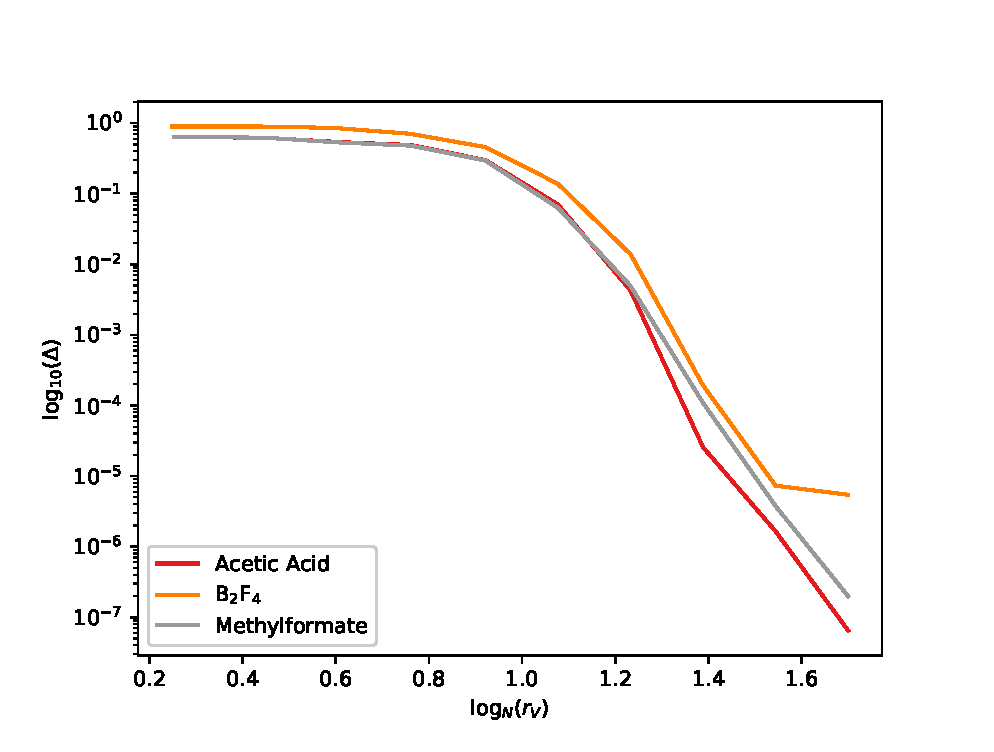
\includegraphics[width=\columnwidth]{figures/thc_rccsd/mp2_err_ao_full}
\caption{Absolute error in the MP2 correlation energy as the function of rank 
$r_{V}$, H
\label{fig:mp2_err_ao_full}}
\end{figure}
%
\subsection{Accuracy of THC-RCCSD}
We are now ready to evaluate the accuracy of the THC-decomposed RCCSD
method. Recall that we set the rank in the decomposition of amplitudes 
equal to the rank used in the decomposition of two electron integrals. The 
error in the RCCSD correlation energy has a non-monotonic dependence on THC 
rank, but follows the 
same basic trends as seen in Fig.~\ref{fig:thc_err_mo_3systems} and
Fig.~\ref{fig:mp2_err_ao_full}. Similarly to the case of MP2, errors on 
the order of $0.1~mH$ are achieved with $r_\mathrm{T} = r_\mathrm{V} \sim 
N^{1.2} - N^{1.4}$.
%
\begin{figure}[tb]
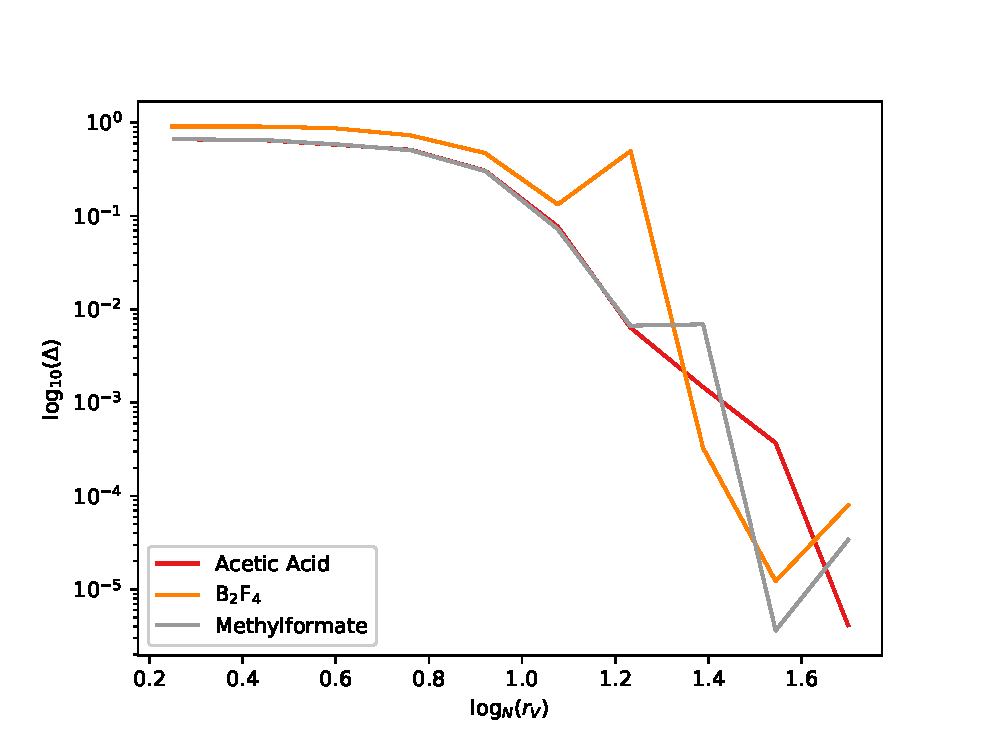
\includegraphics[width=\columnwidth]{figures/thc_rccsd/cc_err_ao_full}
\caption{Absolute error in the RCCSD correlation energy as the function of 
ranks of THC decomposed ${}^2T$ amplitudes and two-electron integrals 
$r_{T} = r_{V}$, H
\label{fig:cc_err_ao_full}}
\end{figure}
%
It is interesting to estimate what part of the error in energy can be
attributed to the approximation of the Hamiltonian only. For this reason we 
calculated the correlation energy with converged THC-RCCSD amplitudes but exact
two-electron integrals.  As Fig.~\ref{fig:cc_err_ao_full_amps_only}
shows, using the exact two-electron integrals substantially decreases the error 
in energy, which later motivated us to look for better ways of decomposing the 
two-electron integrals. The non-monotonic behavior of the error (as compared to 
MP2) can be attributed to the nonlinear nature of the coupled cluster 
equations, which can be quite sensitive to changes in the parameters of the 
Hamiltonian.
%
\begin{figure}[tb]
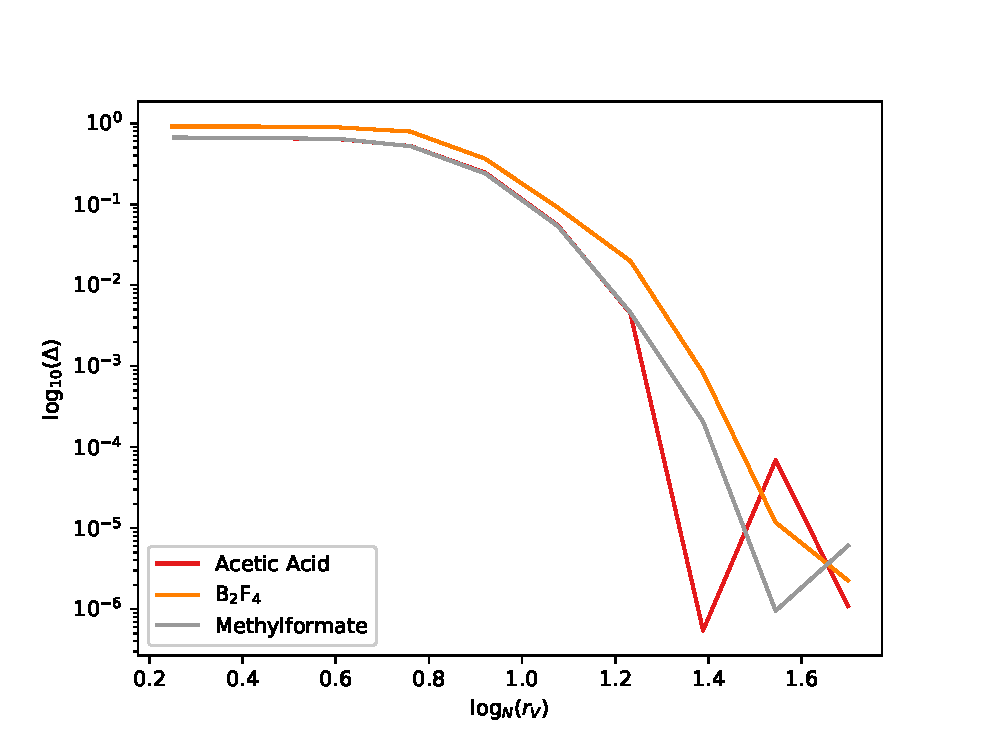
\includegraphics[width=\columnwidth]{figures/thc_rccsd/cc_err_ao_full_amps_only}
\caption{Absolute error in the RCCSD correlation energy with exact two-electron 
integrals and THC decomposed ${}^2T$ amplitudes as a function of rank $r_{T}$, H
\label{fig:cc_err_ao_full_amps_only}}
\end{figure}
%
\subsection{Convergence of THC-RCCSD}
As the solution of THC-RCCSD is found iteratively, an important question is 
the convergence of this method. We used a simple iterative algorithm to 
solve THC-RCCSD equations, and stopped updates when a specified difference in 
energy between subsequent steps was reached. The convergence of the resulting 
method significantly depends on the rank of the THC approximation. 
Figure~\ref{fig:cc_thc_convergence} shows the number of iterations the 
algorithm had to take to reach $10^{6} ~ \mathrm{H}$ difference 
in energy between steps.
%
\begin{figure}[tb]
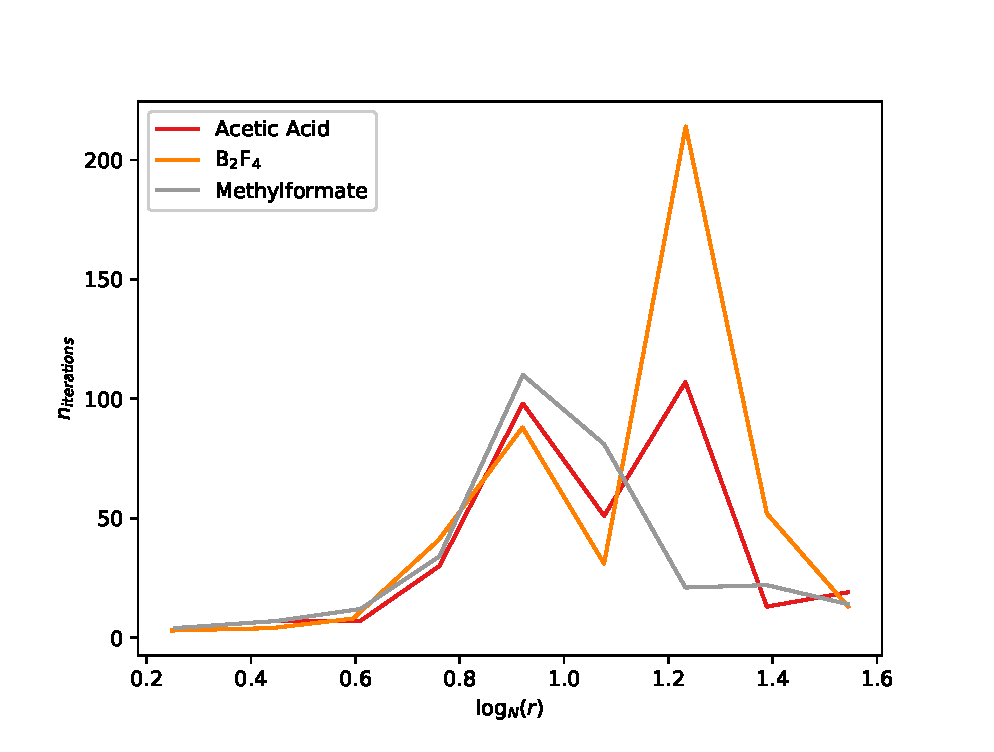
\includegraphics[width=\columnwidth]{figures/thc_rccsd/niter_vs_logr}
\caption{Number of iterations of THC-RCCSD to reach $1 \cdot 10^{-6} H$ 
difference in energy between updates}
\label{fig:cc_thc_convergence}
\end{figure}
%
For small as well as larger THC ranks the convergence of THC-RCCSD is 
comparable or better than regular RCCSD (if solved by simple iteration). 
In the intermediate regime, however, the algorithm may need
a large number of iterations or fails to converge. We note that the 
convergence in this regime significantly depends on the choice of initial 
parameters. This behavior can possibly be explained by the fact that THC-RCCSD 
in our formulation is a sum of two iterative algorithms, namely, an ALS step 
and 
a CC iteration. These two parts of THC-RCCSD can generate competing updates, 
depending on the magnitude of the rank. In case of small ranks the update 
should be mostly determined by ALS, as ${}^{2}T$ amplitudes are poorly 
approximated with any set of parameters $Y$. In contrast, with larger ranks 
mostly the CC step dominates the update, because ${}^2T$ is well 
approximated at each step. We admit, however, that the means to control 
convergence of our hybrid algorithms may need further study. All of the 
calculations in Table~\ref{tab:energies_thc_rccsd} were done in a regime where 
THC-RCCSD performs similarly to regular RCCSD, e. g. where THC ranks are 
relatively large. 

\subsection{{THC-RCCSD for weakly correlated systems}
\label{sec:thc_weakly_correlated}}
Having checked the properties of THC-RCCSD on a few small systems, we 
tested the method on a larger set of small and medium-sized molecules introduced 
in previous work on THC.\cite{hohenstein_thc3} Technical details of the 
calculations, including molecular geometries and reference energies, are 
provided in the supplementary materials of Ref.~\cite{schutski2017tensor}. We 
chose the ranks of the THC decomposition of the amplitudes and integrals to be 
on the same scale as the number of auxiliary basis functions $N_\mathrm{RI}$ 
used in the standard RI approximation. In Table~\ref{tab:energies_thc_rccsd} we 
list 
energies, differences with respect to regular Coupled Cluster and the norm of 
final residuals. We used RI for all these calculations 
in the first step of THC decomposition of the two electron integrals. 
%
\begin{center}
\begin{table}[!ht]
\caption{Tests of the accuracy of THC-RCCSD. CCSD correlation energies ($E_c$), 
errors in correlation energies ($\Delta E_c$) and the norm of doubles residuals 
($|{}^2R_{ij}^{ab}|$) for several  
molecular systems. 
\label{tab:energies_thc_rccsd}}
\begin{tabular}{lccccc}
\hline \hline
& & \multicolumn{2}{c}{$\Delta E_c (mH)$} & 
\multicolumn{2}{c}{$|{}^2R_{ij}^{ab}|$}\\
\cline{3-4} \cline{5-6} System & $E_c (mH)$ & $N_\mathrm{RI}$ &
$1.5 \, N_\mathrm{RI}$ & $N_\mathrm{RI}$ &
$1.5 \, N_\mathrm{RI}$\\
\hline
Acetic acid & -666.510 & -0.579 & -0.453 & 0.041 & 0.033 \\
Aniline & -997.193 & -1.177 & -0.471 & 0.051 & 0.032 \\
Diboron tetrafluoride & -909.944 & -0.702 & -0.716 & 0.053 & 0.034\\
Benzene & -823.101 & -0.985 & -0.450 & 0.048 & 0.030\\
Butadiene & -581.340 & -0.710 & -0.274 & 0.041 & 0.025\\
Cyclobutane & -621.099 & -0.895 & -0.290 & 0.039 & 0.028\\
Dimethylsulfoxide & -661.870 & 0.195 & -0.624 & 0.056 & 0.025\\
Furan & -736.463 & -0.865 & -0.454 & 0.046 & 0.033\\
Isobutane & -652.505 & -0.876 & -0.263 & 0.035 & 0.025\\
Methylformate & -666.805 & -0.586 & -0.455 & 0.042 & 0.032\\
Methylnitrite & -708.990 & -0.476 & -0.492 & 0.047 & 0.033\\
Phenol & -1005.727 & -0.887 & -0.514 & 0.051 & 0.032\\
Pyridine & -842.453 & -1.045 & -0.475 & 0.047 & 0.032\\
Pyrrole & -727.051 & -0.855 & -0.407 & 0.045 & 0.032\\
Thiophene & -695.593 & -1.013 & -0.657 & 0.039 & 0.032\\
Toluene & -980.030 & -1.270 & -0.461 & 0.063 & 0.042\\
\hline
mean unsigned error & & 0.820 & 0.466 & &\\
maximum unsigned error & & 1.270 & 0.716 & &\\
root-mean-square error & & 0.861 & 0.482 & &\\
\hline\hline
\end{tabular}
\end{table}
\end{center}
%
As the table shows, already with moderate ranks on the order of the basis size 
excellent accuracy is attained (differences are below $1 ~ \mathrm{mH}$). The 
error of the approximation decreases as we increase the rank. Let us 
also point to an important finding in Table~\ref{tab:energies_thc_rccsd}. As 
THC-RCCSD is an approximation to regular CC equations, the full residuals may 
not be zero, because the number of CC equations is usually much larger than the 
number of parameters of THC-RCCSD. An interesting observation is that while 
the norm of the double residuals is not negligible in THC-RCCSD, the errors in 
energy are quite low. This contrasts with conventional CC, where the 
difference of energy during iterations with the converged value  
is of the same order as the norm of the residual. This fact is explored in 
more detail in the next chapter. 

\subsection{Conclusions}
The development of the THC-RCCSD method is our first application of the tensor 
structured coupled cluster approach.\cite{schutski2017tensor} THC-RCCSD provides 
a viable approximation to conventional RCCSD and should be orders of magnitude 
faster per iteration, especially for large basis sizes $N$. 

It should be noted, however, that most of the time in our 
calculations was spent on the decomposition of the Hamiltonian rather
than on the solution of approximated CC equations. 
One way to overcome this problem is to use quadrature based methods for 
building THC of the electron interaction tensor, such as the ones developed by 
the group of Martinez.\cite{hohenstein_thc1},\cite{parrish2013discrete} These 
methods may be much faster than iterative approaches we employed, at the 
expense of using about 3x larger ranks to reach the same 
accuracy.\cite{parrish2013discrete} Another way is to avoid THC decomposition 
of two electron integrals altogether, as we will do in the next
section.

An important aspect not covered in our work on THC-RCCSD here is its behavior 
in the strong correlation regime. As was mentioned earlier, conventional 
restricted 
CC methods fail at strong correlation. We will return to the 
discussion of the strong correlation regime in 
Chapter~\ref{sec:strong_correlation}
\section{CPD-RCCSD method
\label{sec:cpd_rccsd}}
\subsection{Introduction}
Having had success with THC-RCCSD, one may think of other possibilities to 
approximate coupled cluster with tensor decompositions. A major limitation of 
the THC-RCCSD is the need to calculate the decomposition of the Hamiltonian with 
iterative methods. Further, THC decomposition is defined only for four-index 
tensors and there is no natural way to generalize it to the higher order 
tensors, which limits its application in coupled cluster theories with higher 
than double excitation operators. 

Let us consider an alternative choice of factorizations of the Hamiltonian and 
excitation amplitudes, which still allows an effective calculation of the 
RCCSD updates. The two-electron integrals are approximated by an 
RI 
decomposition,\cite{koch2003reduced,harbrecht2012low,weigend2009approximated} 
which can be calculated with low effort and is readily available in 
most electronic structure programs, while doubles amplitudes are defined to 
have CP factorized form of rank $r_{T}$. Diagrammatically, these decompositions 
are:
%
\begin{equation}
\vcenter{\hbox{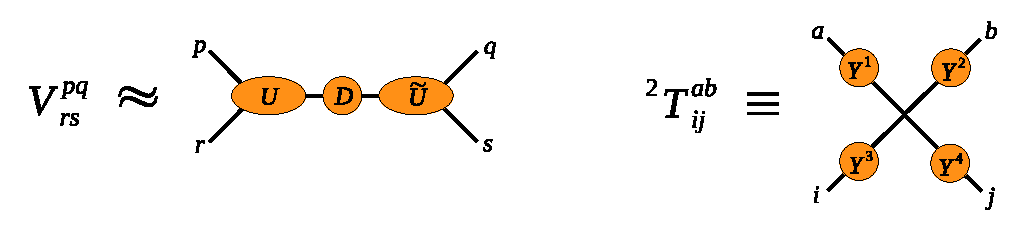
\includegraphics[width=0.9\textwidth]
{figures/cpd_rccsd/rccsd_cpd_def}}}
.
\label{fig:rccsd_cpd_def}
\end{equation}
%
Following the procedure described in Chapter~\ref{ch:tcc}, we derived 
an ALS-like update rule for the factors $Y \in \{Y^{1}, Y^{2}, Y^{3}, Y^{4}\}$. 
We call this method CPD-RCCSD. 
After defining proper intermediates with an automated algebraic 
system,\cite{drudge2} the cost of iteration in CPD-RCCSD is quartic in the 
basis size, auxiliary basis size and $r_{T}$.

CP decomposition was applied in the contest of RCCD before by Benedict and 
Auer.\cite{benedict_ccd, benedict_mp2} Although conceptually similar, our 
method significantly differs in the way one solves for the factors $Y$ of 
the ${}^2T$ amplitude and the use of standard RI decomposition of two-electron 
integrals instead of CPD in the mentioned works.

To study the properties of this new method, we apply it here to weakly 
correlated problems used in the evaluation of 
THC-RCCSD,\cite{schutski2017tensor} as well as to weakly correlated Hubbard 
model. 

\subsection{Computational details}
The CPD-RCCSD code is written in Python~\cite{van2007python} on top of the 
PySCF~\cite{sun2017python} electronic structure package. Hartree-Fock 
solutions, as well as two-electron integrals and density fitted integrals were 
provided by PySCF. For molecular systems we used the standard cc-pVDZ basis set 
from the EMSL database,\cite{schuchardt2007basis} along with the cc-pVDZ-jkfit 
for RI decomposition. In the case of the Hubbard 
Hamiltonian~\ref{sec:hubbard_hamiltonian}
the RI decomposition was built analytically.

For simulations of molecules in Table~\ref{tab:energies_cpd_rccsd} CC iterations 
were stopped after energy converged to within $10^{-6}~\mathrm{H}$ or a limit 
of 500 iterations was reached. In the case of Hubbard Hamiltonian we used a 
threshold of $10^{-12}~\mathrm{t}$ for the energy and 2000 iterations.

\subsection{Exact representations of the Hubbard interaction tensor}
To test the properties of CPD-RCCSD, we employed weakly correlated 
Hubbard models (see Section~\ref{sec:hubbard_hamiltonian}). 
The convenience of the Hubbard Hamiltonian is that the two-body interaction term 
in the on-site basis has simple structure. The full 4-index interaction in a 
model with $N$ sites is a diagonal tensor of size $N\times N\times N \times N$, 
having $\eta$ on the diagonal. Exact representations of the Hubbard interaction 
tensor in various forms can be easily built.

The exact RI representation ($V_{pqrs} = 
\eta \sum_{\alpha} U_{pr\alpha} \tilde{U}_{qs\alpha}$) of the Hubbard 
interaction has rank $N$. Tree index RI factors can be chosen to be sparse $N 
\times N \times N$ tensors with elements $U_{ij\alpha} = \tilde{U}_{ij\alpha} 
= \delta_{i}^{\alpha} \delta_{j}^{\alpha} \cdot \sqrt{\eta}$. Likewise, an 
exact THC decomposition ($V_{pqrs} = \eta \sum_{\alpha \beta} W^{1}_{p\alpha} 
W^{2}_{r\alpha} X_{\alpha, \beta} W^{3}_{q\beta} W^{4}_{s\beta}$) has ranks 
equal $N$, and matrices $W \in \{W^{1}, W^{2}, W^{3}, W^{4}, X\}$ are identity 
matrices of size $N \times N$. The scalar $\eta$ can be absorbed into the 
matrix $X$. Finally, an exact CP decomposition ($V_{pqrs} = \eta \sum_{\alpha} 
W^{1}_{p\alpha} W^{2}_{r\alpha} W^{3}_{q\alpha} W^{4}_{s\alpha}$) has rank $N$.
Factor matrices, as previously, are identities. Summarizing, all decompositions 
of the Hamiltonian considered in this work can be built exactly and have low 
ranks. In Hubbard model calculations the approximations, thus, affect only 
cluster amplitudes.

\subsection{CPD-RCCSD in weakly correlated systems}
We first use CPD-RCCSD to calculate energy of the Hubbard model.
The energies of $6$-, $10$-, $14$- and $18$-site periodic Hubbard systems at 
half-filling were calculated at $\eta = 2$.
%
\begin{figure}[!tb]
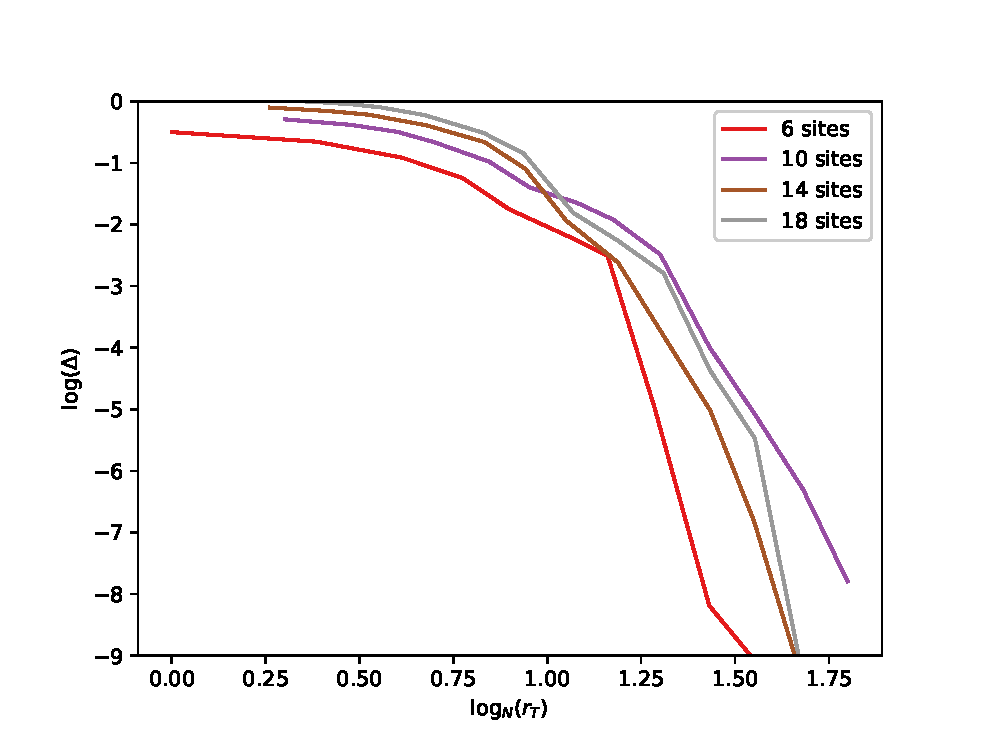
\includegraphics[width=\columnwidth]{figures/cpd_rccsd/err_vs_r_u_2_cpd}
\caption{Absolute error in correlation energy per site for the 
Hubbard model at $\eta = 2$ as the function of rank $r_{T}$ of CP decomposed
${}^2T$ amplitudes, H
\label{fig:err_vs_r_u_2}}
\end{figure}
%
As the graph demonstrates, the difference in the correlation energy 
between CPD-RCCSD and conventional RCCSD methods decays exponentially as the 
rank $r_{T}$ is increased, similarly to the THC-RCCSD method. At  
$r_{T} \sim N^{1.2} - N^{1.5}$ the difference induced by the decomposition 
of doubles amplitudes is less than $10^{-3}~\mathrm{t}$, which an excellent 
approximation of RCCSD. 

To further assess the performance of CPD-RCCSD, we computed the energy 
of a set of molecules previously used for evaluating THC-RCCSD. The magnitude 
of $r_{T}$ is chosen to be a multiple of the size of the auxiliary basis used 
in the RI decomposition of the Hamiltonian.
%
\begin{center}
\begin{table}[!ht]
\caption{CCSD correlation energies ($E_c$), errors in
correlation energies ($\Delta E_c$)
and the norm of doubles residuals ($|{}^2R_{ij}^{ab}|$) for several small 
molecules.
\label{tab:energies_cpd_rccsd}}
\begin{tabular}{lccccccc}
\hline \hline
& & \multicolumn{2}{c}{$\Delta E_c~(mH)$} & 
\multicolumn{2}{c}{$|{}^2R_{ij}^{ab}|$}\\
\cline{3-4} \cline{5-6} System & $E_c~(mH)$ & $1.5 \, N_\mathrm{RI}$ &
$2 \, N_\mathrm{RI}$ & $1.5 \, N_\mathrm{RI}$ &
$2 \,~N_\mathrm{RI}$\\
\hline
AceticAcid & -228.506 & 5.955 & 3.169 & 0.262 & 0.195 \\
Aniline & -286.771 & 14.771 & 7.378 & 0.360 & 0.208 \\
Diboron tetrafluoride & -448.299 & 7.143 & 4.232 & 0.318 & 0.271 \\
Benzene & -231.559 & 11.144 & 5.596 & 0.298 & 0.167 \\
Butadiene & -155.525  & 4.717 & 2.483 & 0.198 & 0.105 \\
Cyclobutane & -156.738  & 5.215 & 2.329 & 0.185 & 0.094 \\
Dimethylsulfoxide & -552.232  & 5.206 & 2.518 & 0.221 & 0.149 \\
Furan & -229.390 & 9.540 & 4.675 & 0.310 & 0.191 \\
Isobutane & -157.973 & 4.187 & 2.242 & 0.124 & 0.087 \\
Methylformate & -228.479 & 6.247 & 3.271 & 0.267 & 0.198 \\
Methylnitrite & -244.398 & 7.112 & 3.856 & 0.290 & 0.209 \\
Pyridine & -247.570 & 11.996 & 6.341 & 0.311 & 0.205 \\
Pyrrole & -209.566 & 9.330 & 4.569 & 0.293 & 0.163 \\
Thiophene & -552.031 & 7.703 & 4.127 & 0.238 & 0.147 \\
Phenol & -306.608 & 14.430 & 7.419 & 0.366 & 0.224 \\
Toluene & -270.758 & 14.333 & 6.706 & 0.355 & 0.171 \\
mean unsigned error & & 8.689 & 4.432 & & &\\
max unsigned error & & 14.771 & 7.419 & & &\\
root-mean-square error& & 9.379 & 4.758 & & &\\
\hline\hline
\end{tabular}
\end{table}
\end{center}
%
The results in Table~\ref{tab:energies_cpd_rccsd} are similar to the results
of THC-RCCSD. As the rank $r_{T}$ is increased, the quality of approximation 
improves. Typical errors are around $5~\mathrm{mH}$ for the rank of CPD of 
doubles amplitudes being twice as large as the size of the auxiliary basis used 
in the decomposition of the Hamiltonian. The errors in CPD-RCCSD are around five 
times higher than in THC-RCCSD for the same rank values. We attribute this to 
the larger number of the parameters in THC-RCCSD, having $4 \cdot N r_{T} + 
r^{2}_{T}$ for parameterizing amplitudes versus $4 \cdot N r_{T}$ in CPD-RCCSD. 
The comparison of Tables~\ref{tab:energies_cpd_rccsd} and 
\ref{tab:energies_cpd_rccsd} shows, however, that the accuracy of CPD-RCCSD 
increases more monotonically with the size of the rank. We suspect that a 
cancellation of errors happens in case of THC-RCCSD because of the more 
complicated approximation to the Hamiltonian, and CPD-based coupled 
cluster provides a more predictable approximation.

\subsection{Conclusions}
To summarize, CPD-RCCSD provides an alternative efficient approximation to the 
coupled cluster with singles and doubles. Overall, CPD-RCCSD and THC-RCCSD 
have a similar accuracy and asymptotic scaling of computational cost. 
Practically, CPD-RCCSD is much faster due to the use of an efficient RI 
decomposition of the electron interaction in place of THC. An additional 
benefit of using canonical decomposition of amplitudes is that the method can 
be further generalized to higher order coupled cluster theories.


\section{Tensor structured CC in strong correlation limit
\label{sec:strong_correlation}}
\subsection{Introduction}
In this section we will discuss the behavior of tensor structured CC methods 
in strong correlation regime, as long as some possible future lines of 
research. As was mentioned in Chapter~\ref{ch:introduction}, strong correlation 
presents a major challenge to current many-body methods. Standard 
coupled cluster methods perform poorly in strong correlation, unless allowed 
to break proper physical symmetries of the wavefunction or very high orders of 
excitation operators are taken into account. Both of the later options are very 
implausible in applications.

The simplest case when strong correlation arises in molecular systems is a 
dissociation of multielectron bonds and various transition state 
configurations. Model Hamiltonians are also a convenient benchmark for 
many-body methods in strong correlation. The eigenstates of the Hubbard 
Hamiltonian at half-filling are strongly correlated when the onsite repulsion is 
significantly higher than the kinetic energy, e.g. $\eta = U / t \gg 1$. We 
used these two settings to test the behavior of tensor structured coupled 
cluster methods.

\subsection{Rank restriction in TCC at strong correlation}
As a first test, we applied CPD-RCCSD to Hubbard models with 6, 10 and 14 
sites. 
%
\begin{figure}[ht!]
\centering
%\begin{subfigure}{0.75\textwidth}
%\centering
%\includegraphics[width=1\linewidth]
%{figures/tcc_strong_correlation/energy_vs_u_6_sites_cpd_rccsd}
%\caption{6 sites}
%\label{fig:energy_vs_u_6_sites_cpd_rccsd}
%\end{subfigure}
%\begin{subfigure}{0.75\textwidth}
%\centering
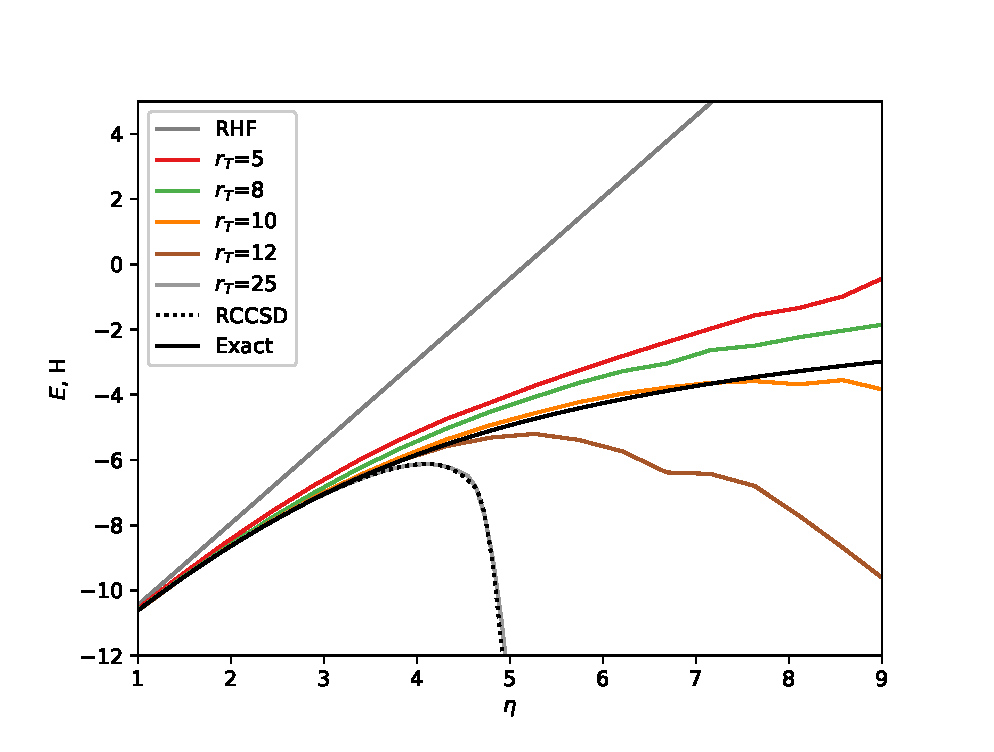
\includegraphics[width=\columnwidth]
{figures/tcc_strong_correlation/energy_vs_u_10_sites_cpd_rccsd}
%\caption{10 sites}
%\label{fig:energy_vs_u_10_sites_cpd_rccsd}
%\end{subfigure}
\caption{Energy behavior for different ranks of CP decomposition of amplitudes. 
Hubbard model at half-filling, 10 sites}
\label{fig:energy_vs_u_cpd}
\end{figure}
%
Figure~\ref{fig:energy_vs_u_cpd} shows the dependence of the total energy 
on the interaction strength $\eta$. As expected, conventional RCCSD provides 
good description of Hubbard rings at low $\eta$, and systematically 
overestimates the energy as the system becomes strong correlated. CPD-RCCSD, 
however, demonstrates a surprising effect. If one chooses the approximation to 
doubles amplitudes to be low 
rank, the incorrect behavior of the original RCCSD method may be fixed. As the 
rank in increased, the solutions of CPD-RCCSD gradually change behavior between 
the one of Hartree-Fock (no correlation) to conventional RCCSD 
(overestimation of correlation energy), as can be seen on 
Figure~\ref{fig:energy_vs_u_cpd}. This situation, however, is not 
specific to CPD-RCCSD, and is also observed with THC-RCCSD (see 
Figure~\ref{fig:energy_vs_u_thc}).
%
\begin{figure}[ht!]
\centering
%\begin{subfigure}{0.75\textwidth}
%\centering
%\includegraphics[width=1\linewidth]
%{figures/tcc_strong_correlation/energy_vs_u_6_sites_thc_rccsd}
%\caption{6 sites}
%\label{fig:energy_vs_u_6_sites_thc_rccsd}
%\end{subfigure}
%\begin{subfigure}{0.75\textwidth}
%\centering
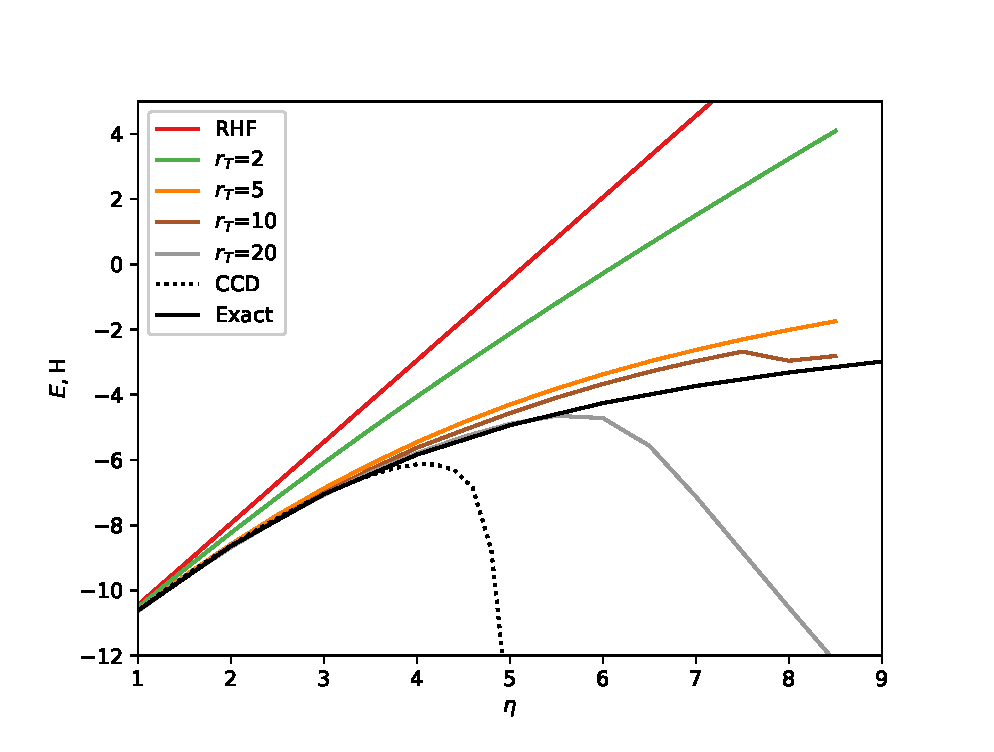
\includegraphics[width=\columnwidth]
{figures/tcc_strong_correlation/energy_vs_u_10_sites_thc_rccsd}
%\caption{10 sites}
%\label{fig:energy_vs_u_10_sites_thc_rccsd}
%\end{subfigure}
\caption{Energy behavior for different ranks of THC decomposition of 
amplitudes. Hubbard model at half-filling, 10 sites}
\label{fig:energy_vs_u_thc}
\end{figure}
%
The difference in case of THC-RCCSD is that the overcorrelation happens at 
slightly larger ranks (compare, for example, $r_{T} = 5$ and $r_{T} = 10$ 
between Figures~\ref{fig:energy_vs_u_cpd} and \ref{fig:energy_vs_u_thc}). Both 
methods, however, reproduce standard RCCSD when sufficiently large ranks of the 
decompositions are chosen, as one may expect.

The results observed with Hubbard Hamiltonian do not change qualitatively in 
case of molecular systems. Figure~\ref{fig:energy_vs_d_cc-pvdz} 
demonstrates the effect of rank restriction in CPD-RCCSD for the calculation of 
the dissociation curve of nitrogen. With rank equal 4 the solution has a 
correct behavior at the dissociation limit, while for larger ranks CPD-RCCSD 
approximates standard RCCSD. The rank restricted solutions, however, miss a 
fair amount of weak correlation energy (e.g. near the equilibrium exact and 
CPD-RCCSD curves are far apart), which plays a major role in molecular systems. 
Having seen the behavior of rank restricted approximate coupled cluster for a 
wide range of systems, we would like to provide an interpretation of the 
observed effect.
%
\begin{figure}[!ht]
\centering
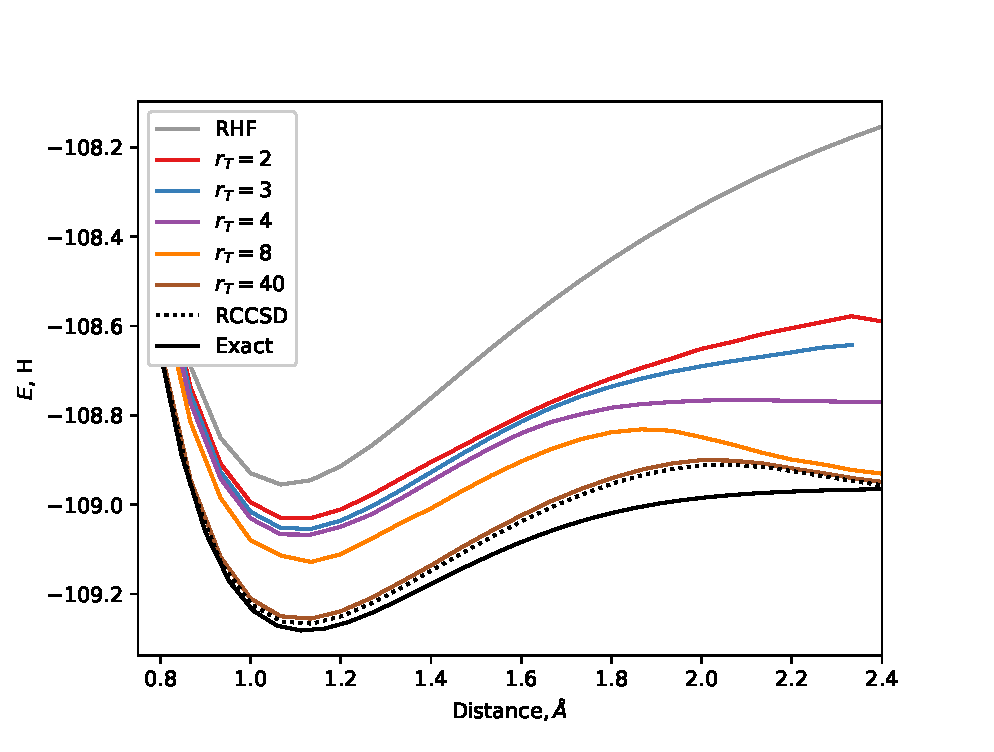
\includegraphics[width=\columnwidth]
{figures/tcc_strong_correlation/energy_vs_d_cc-pvdz}
\caption{Dissociation of nitrogen. CPD-RCCSD energies with different ranks 
$r_{T}$ in amplitude approximation}
\label{fig:energy_vs_d_cc-pvdz}
\end{figure}
%

\subsection{Tentative explanation}
To explain the observed effect one may look at 
different parameters of CPD-RCCSD solutions. In 
Figure~\ref{fig:t2_norms_vs_u_10_sites_cpd_rccsd} the dependence of the norm of 
the 
${}^2T$ amplitudes as a function of rank and on-site repulsion is shown. As the 
graph illustrates, the norm of the doubles amplitudes in the physically 
proper-behaving low rank solutions is lower than the norm of ${}^2T$ amplitudes 
in conventional RCCSD. In contrast, as the ranks grow and CPD-RCCSD starts 
to overcorrelate there is a sharp increase in the amplitude norm to values even 
higher than the standard RCCSD would yield. For example, the solution with 
$r_{T} = 12$, which significantly overcorrelates at $\eta > 6$ (see 
Figure~\ref{fig:energy_vs_u_cpd}, yellow line) also has large 
norm of ${}^2T$ amplitudes starting at the same values of $\eta$ 
(Figure~\ref{fig:t2_norms_vs_u_10_sites_cpd_rccsd}, yellow line). 
The growth of cluster amplitudes was identified as the major problem of the CC 
\emph{ansatz} at strong correlation.\cite{degroote2016polynomial}
%
\begin{figure}[ht]
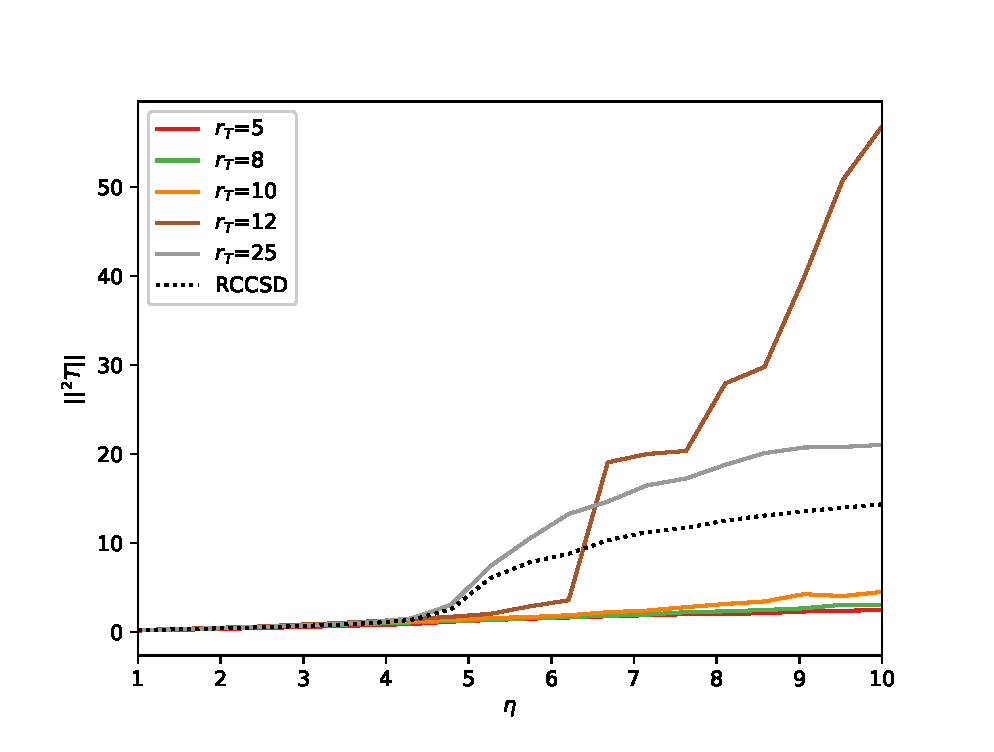
\includegraphics[width=\columnwidth]
{figures/tcc_strong_correlation/t2_norms_vs_u_10_sites_cpd_rccsd}
\caption{Norm of ~ ${}^2T$ amplitudes for different ranks $r_{T}$ in CPD-RCCSD 
calculations. Hubbard model at half-filling, 10 sites.
\label{fig:t2_norms_vs_u_10_sites_cpd_rccsd}}
\end{figure}
%
It was demonstrated by M. Degroote\emph{et al.}~\cite{degroote2016polynomial} 
that in strong correlation regime the magnitude of amplitudes of higher order 
(e.g. triples, quadruples, etc.) in standard restricted CC increases with 
the rank of excitation.

Since CC theory uses an exponential parameterization 
of the wavefunction, e.g. $|\phi \rangle = e^{T} | 0 \rangle$, where $T = {}^1T 
+ {}^2T + {}^3T + \ldots$ (see Chapter~\ref{ch:tcc} for more details), there is 
no natural truncation of the CC excitation operator at strong correlation. 
In a series of works in our group\cite{degroote2016polynomial, 
gomez2017attenuated, qiu2017projected2, hermes2017combining} alternative 
similarity transformations (e.g. non-exponential) were explored, 
which have an excellent accuracy at strong correlation. In those CC-like methods 
the amplitudes do not satisfy the residual equations of standard coupled 
cluster and have smaller norms, which decrease with the order of excitation, due 
to the renormalization of higher order amplitudes. It can be argued that the 
(truncated) exponential \emph{ansatz} of coupled cluster is ill-posed in strong 
correlation setting. By forcing the solution to satisfy CC residual equations 
with excitation operators of low order one makes them significantly deviate from 
the true eigenstates of the Hamiltonian.

It is interesting to note that the low-rank solutions in tensor structured CC 
do not satisfy the CC residual equation either, as 
Figure~\ref{fig:r2_norms_vs_u_10_sites_cpd_rccsd} makes clear. The 
individual factors in the decomposition of amplitudes, however, \emph{do} 
satisfy their own ALS-like equations (see Chapter~\ref{ch:tcc}). The CC 
residuals are large for low-rank solutions and sharply drop as 
CPD-RCCSD amplitudes approach regular RCCSD amplitudes (compare $r_{T} = 8$ 
and $r_{T} = 25$ in 
Figures~\ref{fig:energy_vs_u_thc},~\ref{fig:t2_norms_vs_u_10_sites_cpd_rccsd} 
and~\ref{fig:r2_norms_vs_u_10_sites_cpd_rccsd}). Rank restriction of the 
amplitudes can thus be viewed as a way to regularize conventional CC equations 
in strong correlation regime. We would like to point out that similar 
regularization schemes (called "dropout regularization") are ubiquitous in 
machine learning literature.~\cite{srivastava2014dropout, wan2013regularization} 
The latter rises a question whether other regularization approaches, like 
standard $l_{2}$-norm regularization, can be applied in coupled cluster method.
%
\begin{figure}[ht]
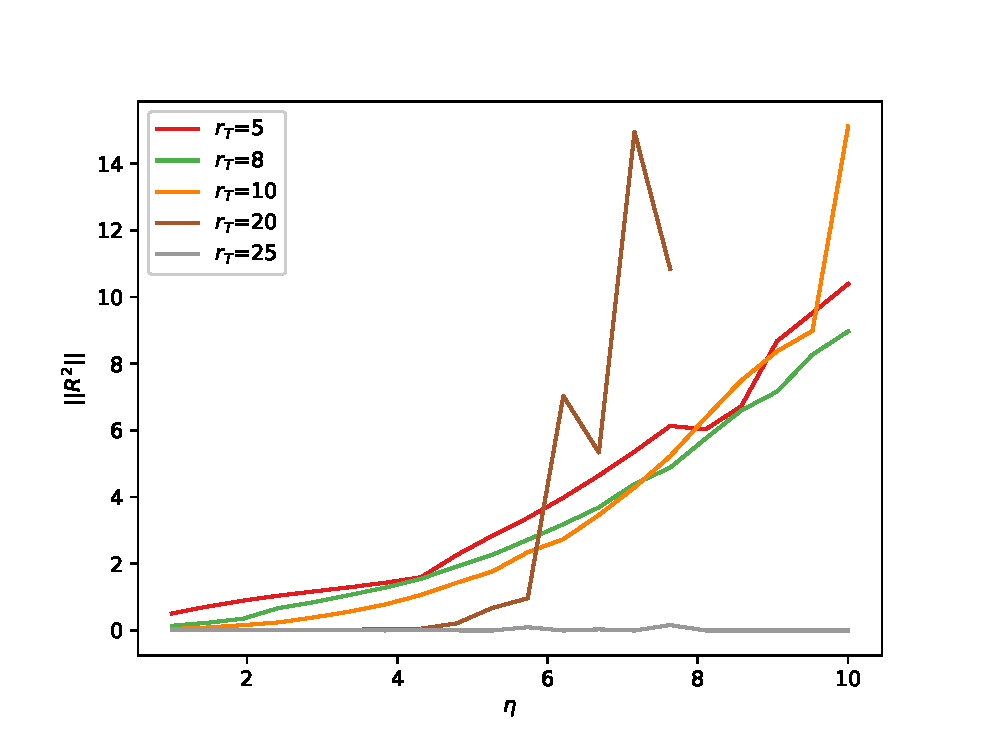
\includegraphics[width=\columnwidth]
{figures/tcc_strong_correlation/r2_norms_vs_u_10_sites_cpd_rccsd}
\caption{Norm of ~${}^2T$ residuals for different ranks $r_{T}$ in CPD-RCCSD 
calculations. Hubbard model at half-filling, 10 sites}
\label{fig:r2_norms_vs_u_10_sites_cpd_rccsd}
\end{figure}
%

\subsection{Conclusions}
The strong correlation regime poses a hard problem for most many-body methods. 
Coupled Cluster methods, while being very effective for weakly correlated 
systems, fail when the strong correlation dominates. Recently a series of 
promising CC-like theories was developed in our 
group.\cite{degroote2016polynomial, gomez2017attenuated, 
qiu2017projected2, hermes2017combining} 
The problem of these theories, however, is that the explicit form of equations 
depends on the symmetry of the Hamiltonian responsible for the onset of strong 
correlation, and the idea is hard to generalize for arbitrary Hamiltonians. On 
the other hand, rank restriction in tensor structured CC provides another way to 
regularize the solutions of standard coupled cluster at strong correlation, 
independently of the form of the Hamiltonian. More research is needed to make 
this approach practically applicable, but we believe the idea may be 
interesting in future method development.
\chapter{Conclusions and outlook
\label{ch:conclusions}}
In this work two new approximate coupled cluster methods were developed. Our 
approach is based on tensor decompositions, which are alternative 
representations of high dimensional tensors ubiquitous in post-Hartree-Fock 
theories. After an introduction into the theory of coupled cluster is done, we 
focus on three tensor formats employed in this work: resolution of 
identity (RI), canonical polyadic decomposition (CPD) and tensor 
hypercontraction (THC). We represent mentioned tensor formats in a uniform way 
with the help of tensor diagrams and discuss techniques to cast different 
index-based tensors into CPD and THC forms. 

While higher order tensors are approximated with tensor decompositions, the 
decisive quantity is the length of the expansion (the rank). The cost of 
tensor contractions with decomposed tensors depends on the form of the 
decomposition, the rank(s) $r$ and the basis size $N$. We 
demonstrate that intermediates in coupled cluster can be calculated at 
cost scaling as the 4-th power of $r$ and $N$. The discussion culminates by 
the derivation of a general tensor structured coupled cluster method using THC 
factorization as an example. In our approach the Alternating Least Squares 
procedure is combined with the coupled cluster update to produce a new 
iterative algorithm for the factors of the decomposed cluster amplitudes. This 
generic algorithm has quartic cost per iteration if the THC or the CPD 
factorization is used for the amplitude tensors.

After establishing a general framework for tensor structured coupled cluster, 
we present its first concrete realization, namely THC-RCCSD. We demonstrate 
that only small ranks of order $N^{1.3}$ in the THC decomposition of two-body 
interaction are sufficient for sub-mHartree accuracy in MP2 energy, and 
that the quality of the decomposition does not depend significantly on the 
choice of the basis. After combining THC factorized two-body interaction with 
THC factorized amplitudes, we demonstrate that only small ranks of order 
$N^{1.3}$ are needed for the sub-mHartree accuracy of the resulting THC-RCCSD 
method. Provided these findings, the overall scaling of THC-RCCSD is of order 
$O(N^{5})$ for sub-mHartree accuracy, whereas the original RCCSD method has 
$O(N^{6})$ computational cost. The method is tested on a large set of organic 
molecules.   

We then introduce another combination of tensor decompositions to approximate 
RCCSD. The two-body interaction is represented in a standard RI form, 
while cluster amplitudes are treated in CPD format. The resulting CPD-RCCSD 
procedure again has a quartic cost in the ranks and basis, but also is superior 
to the THC-based method due to the use of the fast RI factorization. We prove 
that the sub-mHartree accuracy is obtained with ranks of order $O(N^{1.3})$, 
and hence the overall cost of CPD-RCCSD is similar to THC-RCCSD. We found that 
the accuracy of CPD-RCCSD is around $5$ times lower than that of THC-based 
method with the same rank, but the number of parameters is much less and 
scales only linearly with rank and $N$. Overall, CPD-RCCSD presents a faster and 
simpler alternative to THC-RCCSD. 

Finally, we have demonstrated that the failure of coupled cluster in strong 
correlation regime can be mitigated by using low rank decompositions of 
cluster amplitudes. We argue that low-rank approximations provide a way to 
regularize ill-posed residual equations and draw analogies from methods 
motivated by similar ideas. The later provides a direction for future 
research.

As the framework we developed is quite general, many extensions are possible. 
Tensor structured coupled cluster can be directly applied to unrestricted or 
generalized coupled cluster theories. The mentioned methods work for strongly 
correlated molecular systems at the expense of breaking the spin symmetry of 
the wavefunction. CPD-RCCSD can be directly generalized to the higher orders of 
coupled cluster theory, for example CCSDT, CCSDTQ, CCSDTQ5, where much larger 
numerical savings may be obtained. Additionally, the techniques we describe 
can be used in other CC-like approaches, such as the perspective polynomial 
similarity transformation methods.\cite{degroote2016polynomial, 
gomez2017attenuated} Finally, the regularizing effect of 
low-rank amplitudes calls for the study of regularization methods in the 
coupled cluster approach.
\appendix

%\include{append-a}
%\appendix
%\addcontentsline{toc} {chapter}{\numberline {}Appendix A}  
%\include{append-a}
%\include{append-b}
%\addcontentsline{toc} {chapter}{\numberline {}Bibliography}{}
%\include{biblio}

\bibliographystyle{ieeetr}
\bibliography{references}
\end{document}
